\documentclass[12pt,a4paper]{article}

\usepackage[utf8]{inputenc}
\usepackage[T1]{fontenc}
\usepackage[czech]{babel}
\usepackage{lmodern}
\usepackage{graphicx}
\usepackage{float}
\usepackage{hyperref}
\usepackage{geometry}
\usepackage{xcolor}
\usepackage{tcolorbox}
\usepackage{parskip}
\usepackage{fancyhdr}
\usepackage{titlesec}
\usepackage[font=small,labelfont={bf,color=primaryblue},labelsep=space]{caption}

\geometry{margin=2.5cm, headheight=15pt}

% Color definitions
\definecolor{primaryblue}{RGB}{25, 118, 210}
\definecolor{darkblue}{RGB}{13, 71, 161}
\definecolor{lightbg}{RGB}{245, 247, 250}
\definecolor{accentblue}{RGB}{227, 242, 253}

\hypersetup{
    colorlinks=true,
    linkcolor=primaryblue,
    urlcolor=primaryblue,
    pdftitle={Czech Salivary Gland Database --- Uživatelská příručka},
    pdfauthor={Západočeská univerzita v Plzni}
}

% Section styling
\titleformat{\section}
  {\Large\bfseries\color{darkblue}}
  {\thesection}{1em}{}[\color{primaryblue}\titlerule]

\titleformat{\subsection}
  {\large\bfseries\color{primaryblue}}
  {\thesubsection}{1em}{}

\titleformat{\subsubsection}
  {\normalfont\bfseries\color{darkblue}}
  {\thesubsubsection}{1em}{}

% Header and Footer setup
\pagestyle{fancy}
\fancyhf{}
\fancyhead[L]{\small\color{gray}\textbf{CSGDB} --- Uživatelská příručka}
\fancyhead[R]{\small\color{gray}\leftmark}
\fancyfoot[L]{\small\color{gray}Západočeská univerzita v Plzni}
\fancyfoot[R]{\small\color{gray}\thepage}
\renewcommand{\headrulewidth}{0.4pt}
\renewcommand{\footrulewidth}{0.4pt}

\begin{document}

% Custom Title Page
\begin{titlepage}
    \pagenumbering{alph}
    \pagecolor{white}
    \fontfamily{lmss}\selectfont
    \centering
    
    \vspace*{1.5cm}
    
    % Banner Logo
    
\includegraphics[width=0.85\textwidth]{img/LOGO_splt.png}
    
    \vspace{2cm}
    
    {\Huge \bfseries \color{darkblue} UŽIVATELSKÁ PŘÍRUČKA} \\[0.8em]
    {\Large \color{gray} Databázový a analytický systém pro evidenci a analýzu pacientů s~nádory slinných žláz}
    
    \vspace{1.5cm}
    
    \begin{tcolorbox}[colback=accentblue,colframe=primaryblue,arc=4pt,halign=center,width=0.6\textwidth]
        \centering \Large \bfseries \color{darkblue} Verze 3.0.9
    \end{tcolorbox}
    
    \vfill
    
    {\large \bfseries \color{darkblue} Západočeská univerzita v Plzni} \\[0.3em]
    {\small \color{gray} Fakulta aplikovaných věd --- Katedra informatiky a výpočetní techniky} \\[0.2em]
    {\small \color{gray} Ve spolupráci s Českou společností otorinolaryngologie a chirurgie hlavy a krku}
    
    \vspace{1cm}
    {\small \color{gray} Plzeň}
    
\end{titlepage}
\nopagecolor

\pagenumbering{arabic}
\pagestyle{fancy}
\tableofcontents
\newpage

\section{Instalace aplikace}

\begin{enumerate}
    \item Stáhněte si nejnovější instalační soubor z~oficiální stránky \href{https://github.com/vjelinekk/CzechSalivaryGlandDB/releases}{GitHub Releases} (případně přímo z~vydání \href{https://github.com/vjelinekk/CzechSalivaryGlandDB/releases/tag/v3.0.9}{v3.0.9}).
    \item Spusťte stažený instalační soubor (název má tvar \texttt{csgdb-X.X.X-Setup.exe}, např. \texttt{csgdb-3.0.9-Setup.exe}).
    \item V~průběhu instalace postupujte podle pokynů v~instalačním okně (viz Obrázek~\ref{fig:instalace}).
    
    \begin{figure}[H]
        \centering
        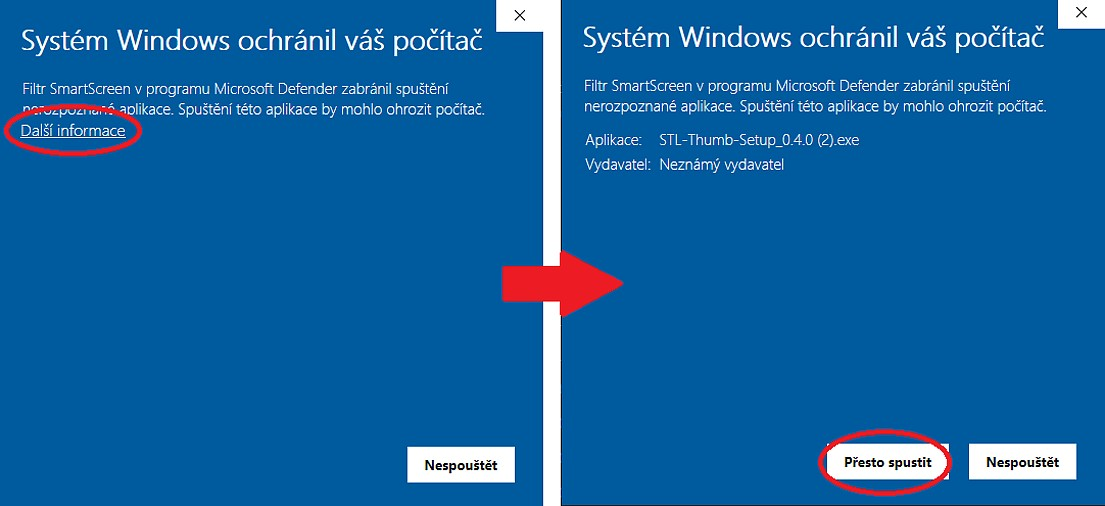
\includegraphics[width=0.8\textwidth]{img/instalace.jpg}
        \caption{Průběh instalace aplikace CSGDB.}
        \label{fig:instalace}
    \end{figure}

    \item Po dokončení instalace je aplikace připravena k~použití a v~systému ji naleznete pod názvem \texttt{csgdb}.
\end{enumerate}

\section{První spuštění aplikace}

\begin{enumerate}
    \item Spusťte aplikaci \texttt{csgdb}.
    \item Při prvním spuštění se zobrazí dialogové okno s~volbou režimu zabezpečení (viz Obrázek~\ref{fig:volba-zabezpeceni}).

    \begin{figure}[H]
        \centering
        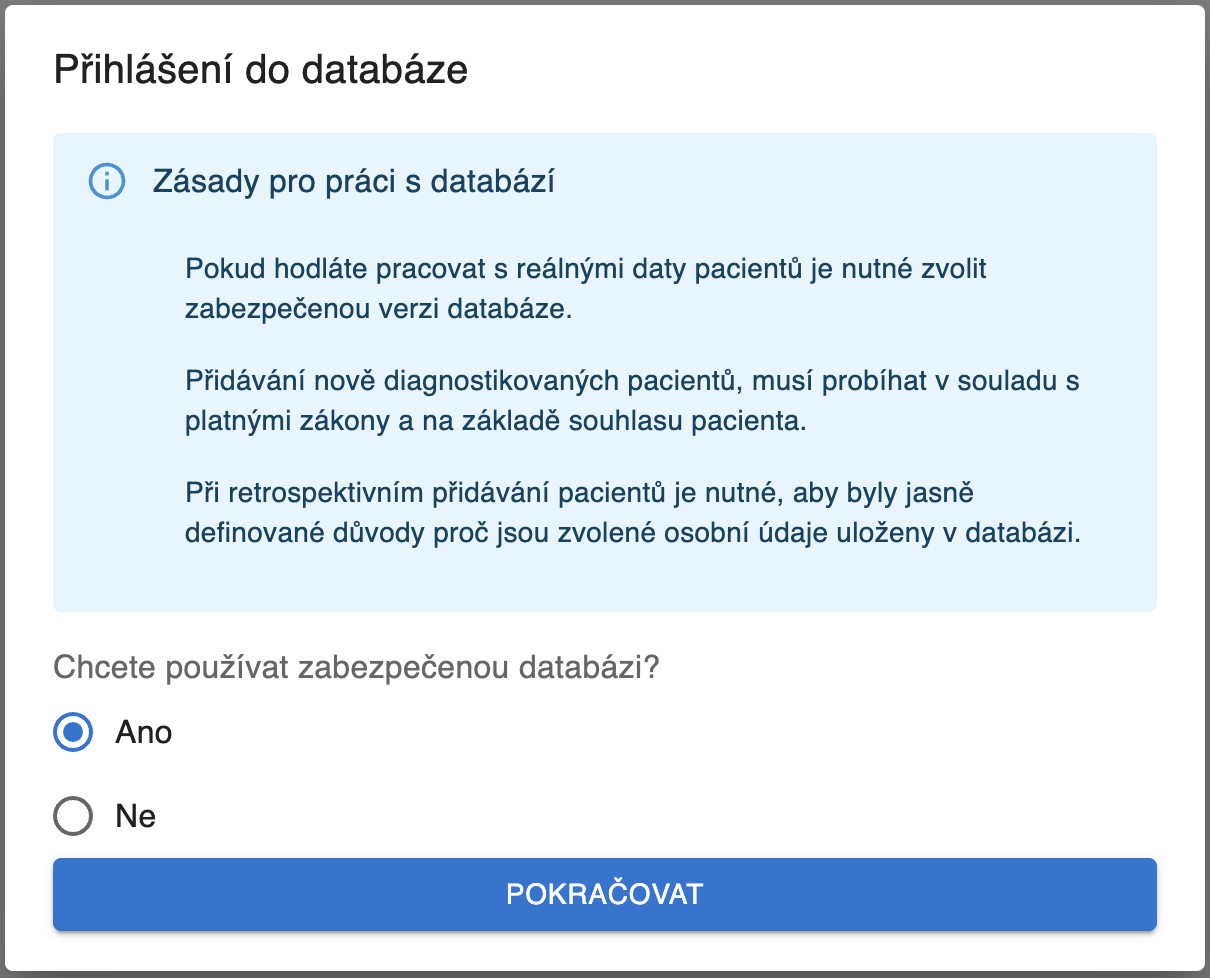
\includegraphics[width=0.8\textwidth]{img/volba_zabezpeceni.png}
        \caption{Volba zabezpečení databáze při prvním spuštění.}
        \label{fig:volba-zabezpeceni}
    \end{figure}

    \item Zvolte požadovaný režim podle plánovaného využití aplikace:
    \begin{itemize}
        \item \textbf{Ano}: Tuto možnost zvolte, pokud plánujete do aplikace ukládat \textbf{reálná data pacientů}. V~tomto režimu jsou citlivé osobní údaje šifrovány.
        \item \textbf{Ne}: Tuto možnost zvolte pouze v~případě, že chcete aplikaci jen testovat a nebudete v~ní uchovávat reálná pacientská data.
    \end{itemize}

    \item Pokud jste zvolili možnost \textbf{Ano}, zobrazí se dialogové okno pro nastavení přihlašovacího hesla a šifrovacího klíče (viz Obrázek~\ref{fig:vytvoreni-hesla}).

    \begin{figure}[H]
        \centering
        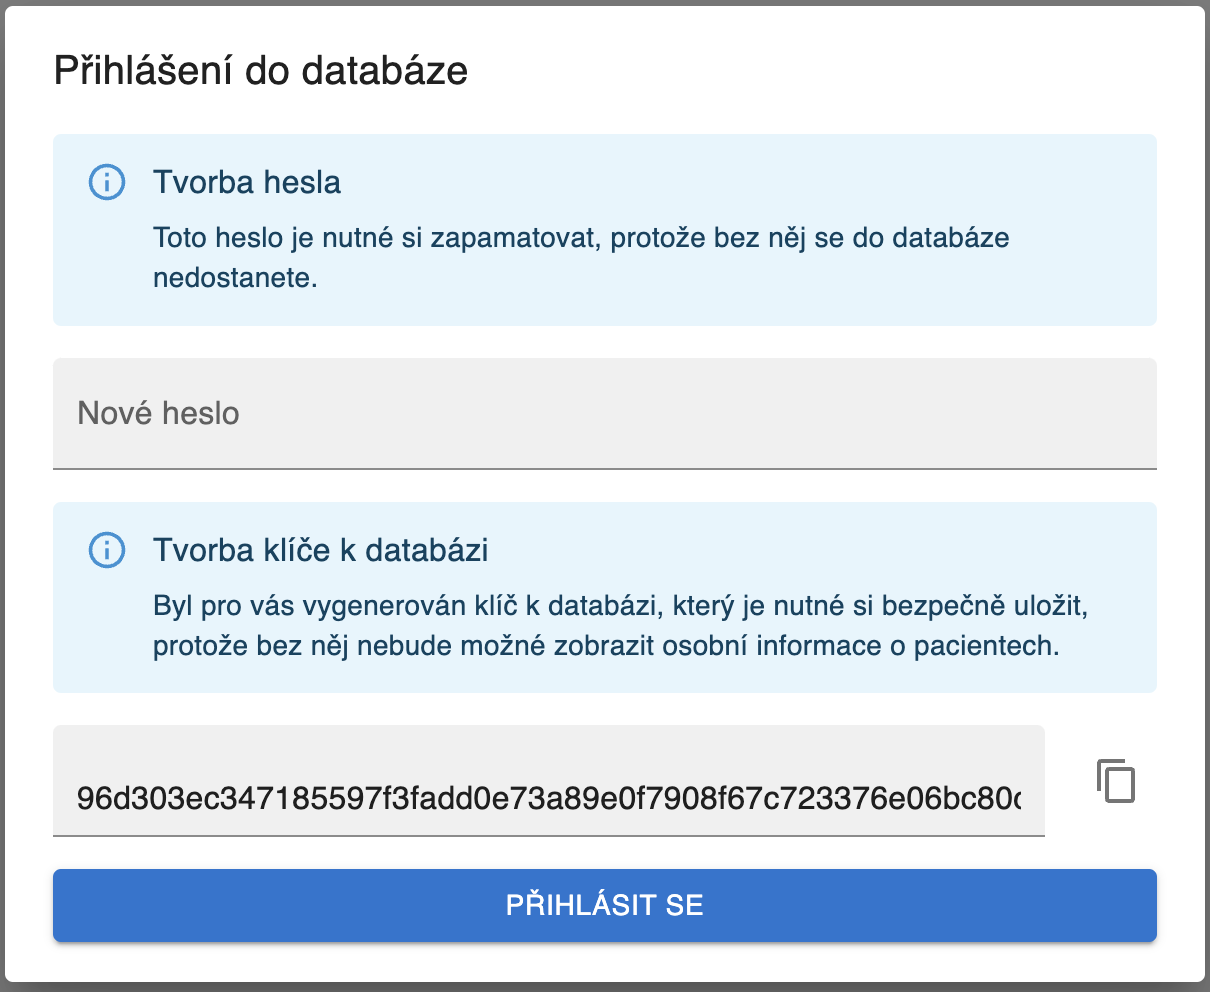
\includegraphics[width=0.8\textwidth]{img/vytvoreni_hesla.png}
        \caption{Nastavení přístupového hesla a vygenerování šifrovacího klíče.}
        \label{fig:vytvoreni-hesla}
    \end{figure}

    \item V~dialogovém okně si nastavte heslo, kterým se budete do aplikace přihlašovat při každém jejím dalším spuštění.
    \item Aplikace pro vás vygeneruje unikátní \textbf{šifrovací klíč}. Ten si uložte nebo zapište na bezpečné místo.
    \item Dokončete nastavení kliknutím na tlačítko \textbf{Přihlásit se}.
\end{enumerate}

\begin{tcolorbox}[colback=red!5!white,colframe=red!75!black,title=\textbf{DŮLEŽITÉ UPOZORNĚNÍ K BEZPEČNOSTI DAT}]
\begin{itemize}
    \item \textbf{Heslo nesmíte zapomenout} -- bez hesla se do aplikace nepřihlásíte a přístup k~uloženým datům bude zablokován.
    \item \textbf{Šifrovací klíč uschovejte na bezpečném místě} -- v~případě ztráty šifrovacího klíče nebude možné dešifrovat a zobrazit osobní údaje o~pacientech.
\end{itemize}
\end{tcolorbox}

\section{Základní popis uživatelského rozhraní}

Uživatelské rozhraní aplikace \texttt{csgdb} je navrženo s~důrazem na přehlednost a intuitivní ovládání. Okno aplikace je rozděleno do tří hlavních částí (viz Obrázek~\ref{fig:rozhrani}):

\begin{figure}[H]
    \centering
    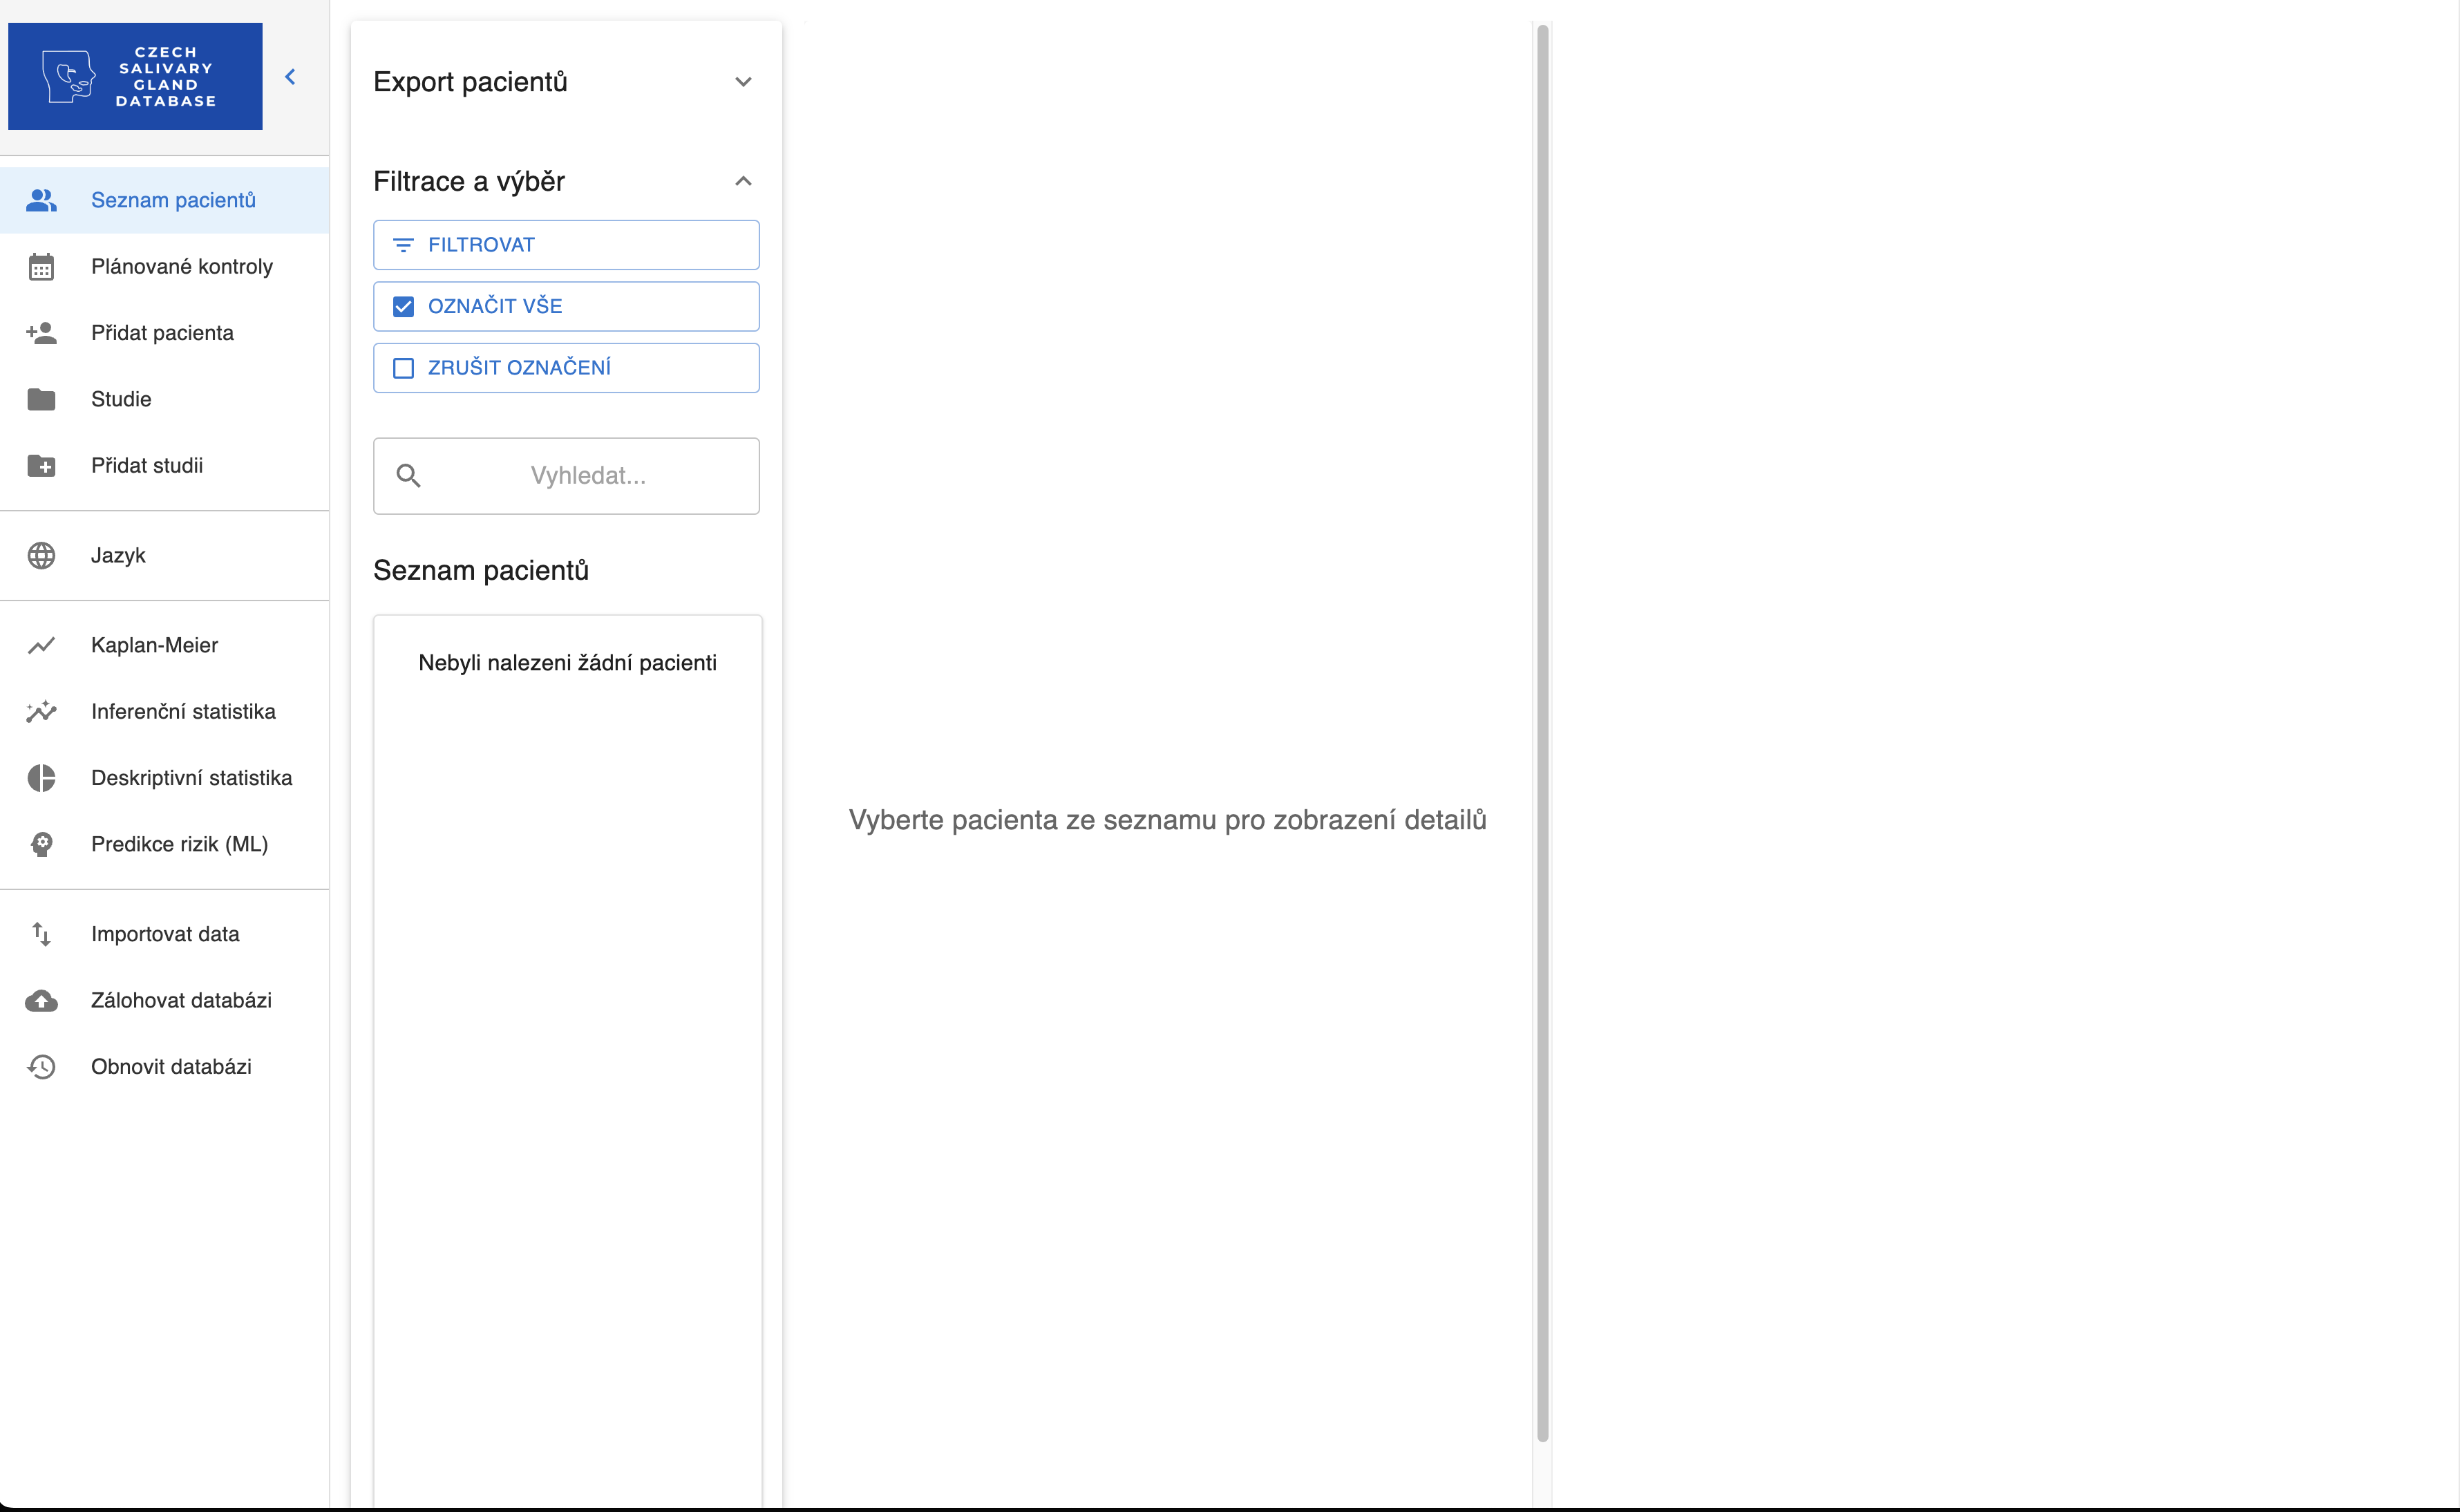
\includegraphics[width=0.95\textwidth]{img/rozhrani.png}
    \caption{Základní rozvržení uživatelského rozhraní aplikace.}
    \label{fig:rozhrani}
\end{figure}

\subsection{Hlavní navigační menu (levý panel)}
Levý postranní panel slouží k~přepínání mezi jednotlivými moduly a funkcionalitami aplikace:

\begin{itemize}
    \item \textbf{Správa pacientů a studií}:
    \begin{itemize}
        \item \textit{Seznam pacientů} -- zobrazí přehled všech evidovaných pacientů s~možností vyhledávání, filtrace a úprav.
        \item \textit{Plánované kontroly} -- přehled plánovaných lékařských kontrol u~pacientů.
        \item \textit{Přidat pacienta} -- formulář pro vložení nového pacienta do databáze.
        \item \textit{Studie} -- přehled a správa klinických studií.
        \item \textit{Přidat studii} -- rozhraní pro vytvoření nové studie a zařazení pacientů do studie.
    \end{itemize}
    
    \item \textbf{Nastavení}:
    \begin{itemize}
        \item \textit{Jazyk} -- přepínání jazyka uživatelského rozhraní (aplikace podporuje českou a anglickou lokalizaci).
    \end{itemize}

    \item \textbf{Analytické a statistické moduly}:
    \begin{itemize}
        \item \textit{Kaplan-Meier} -- vykreslení a analýza křivek přežití a recidivy.
        \item \textit{Inferenční statistika} -- pokročilé statistické testy a porovnání skupin.
        \item \textit{Deskriptivní statistika} -- přehledy základních statistických ukazatelů o~pacientech.
        \item \textit{Predikce rizik (ML)} -- prognostický modul využívající modely strojového učení pro výpočet rizik a trénování nových modelů.
    \end{itemize}

    \item \textbf{Správa dat a databáze}:
    \begin{itemize}
        \item \textit{Importovat data} -- import pacientů ze vnějších souborů.
        \item \textit{Zálohovat databázi} -- vytvoření záložní kopie databáze.
        \item \textit{Obnovit databázi} -- obnova dat ze záložní kopie.
    \end{itemize}
\end{itemize}

Panel lze zmenšit nebo opět rozbalit pomocí tlačítka se šipkou (\texttt{<}) umístěného vedle loga v~levém horním rohu.

\subsection{Ovládací a seznamový panel (střední panel)}
Střední panel se přizpůsobuje vybranému modulu z~navigačního menu. V~základním pohledu \textit{Seznam pacientů} obsahuje:
\begin{itemize}
    \item \textbf{Export pacientů} -- nabídka pro export vybraných dat do formátu Excel (\texttt{.xls}).
    \item \textbf{Filtrace a výběr} -- ovládací tlačítka pro otevření filtračního menu (\textit{FILTROVAT}), hromadné označení pacientů (\textit{OZNAČIT VŠE}) a zrušení vybraných položek (\textit{ZRUŠIT OZNAČENÍ}).
    \item \textbf{Vyhledávací pole} -- umožňuje rychlé vyhledávání pacientů podle jména, příjmení nebo rodného čísla.
    \item \textbf{Seznam pacientů} -- přehledový seznam odpovídajících záznamů v~databázi.
\end{itemize}

\subsection{Hlavní pracovní plocha (pravý panel)}
Pravý panel představuje hlavní pracovní oblast. Zobrazuje detailní obsah odpovídající vybrané akci -- např. kompletní kartu a formulář pacienta, podrobnosti o~studii, grafické výstupy a tabulky analytických modulů nebo dialogová okna pro nastavení. Pokud není vybrána žádná položka, panel zobrazuje instrukci pro výběr záznamu ze seznamu.

\section{Práce s pacienty}

Tato kapitola popisuje správy pacientských záznamů v~databázi -- od vložení nového pacienta přes vyhledávání a úpravu dat až po jejich mazání.

\subsection{Přidávání nového pacienta}

Vložení nového pacienta do databáze probíhá ve třech přehledných krocích v~průvodci záložky \textbf{Přidat pacienta}:

\begin{enumerate}
    \item \textbf{Volba typu nádoru}:
    V~levém navigačním menu klikněte na tlačítko \textbf{Přidat pacienta}. Zobrazí se úvodní obrazovka (viz Obrázek~\ref{fig:pridani-1}), kde zvolíte charakter nádoru:
    \begin{itemize}
        \item \textbf{Nezhoubný nádor} (zelené tlačítko),
        \item \textbf{Zhoubný nádor} (červené tlačítko).
    \end{itemize}

    \begin{figure}[H]
        \centering
        
\includegraphics[width=0.85\textwidth]{img/pridani-pacienta/pridani_1.png}
        \caption{Krok 1: Výběr charakteru nádoru (nezhoubný / zhoubný).}
        \label{fig:pridani-1}
    \end{figure}

    \item \textbf{Výběr postižené žlázy}:
    Po výběru typu nádoru se zobrazí nabídka pro výběr zasažené slinné žlázy (viz Obrázek~\ref{fig:pridani-2}):
    \begin{itemize}
        \item \textbf{Příušní žláza},
        \item \textbf{Podčelistní žláza},
        \item \textbf{Podjazyková žláza}.
    \end{itemize}

    \begin{figure}[H]
        \centering
        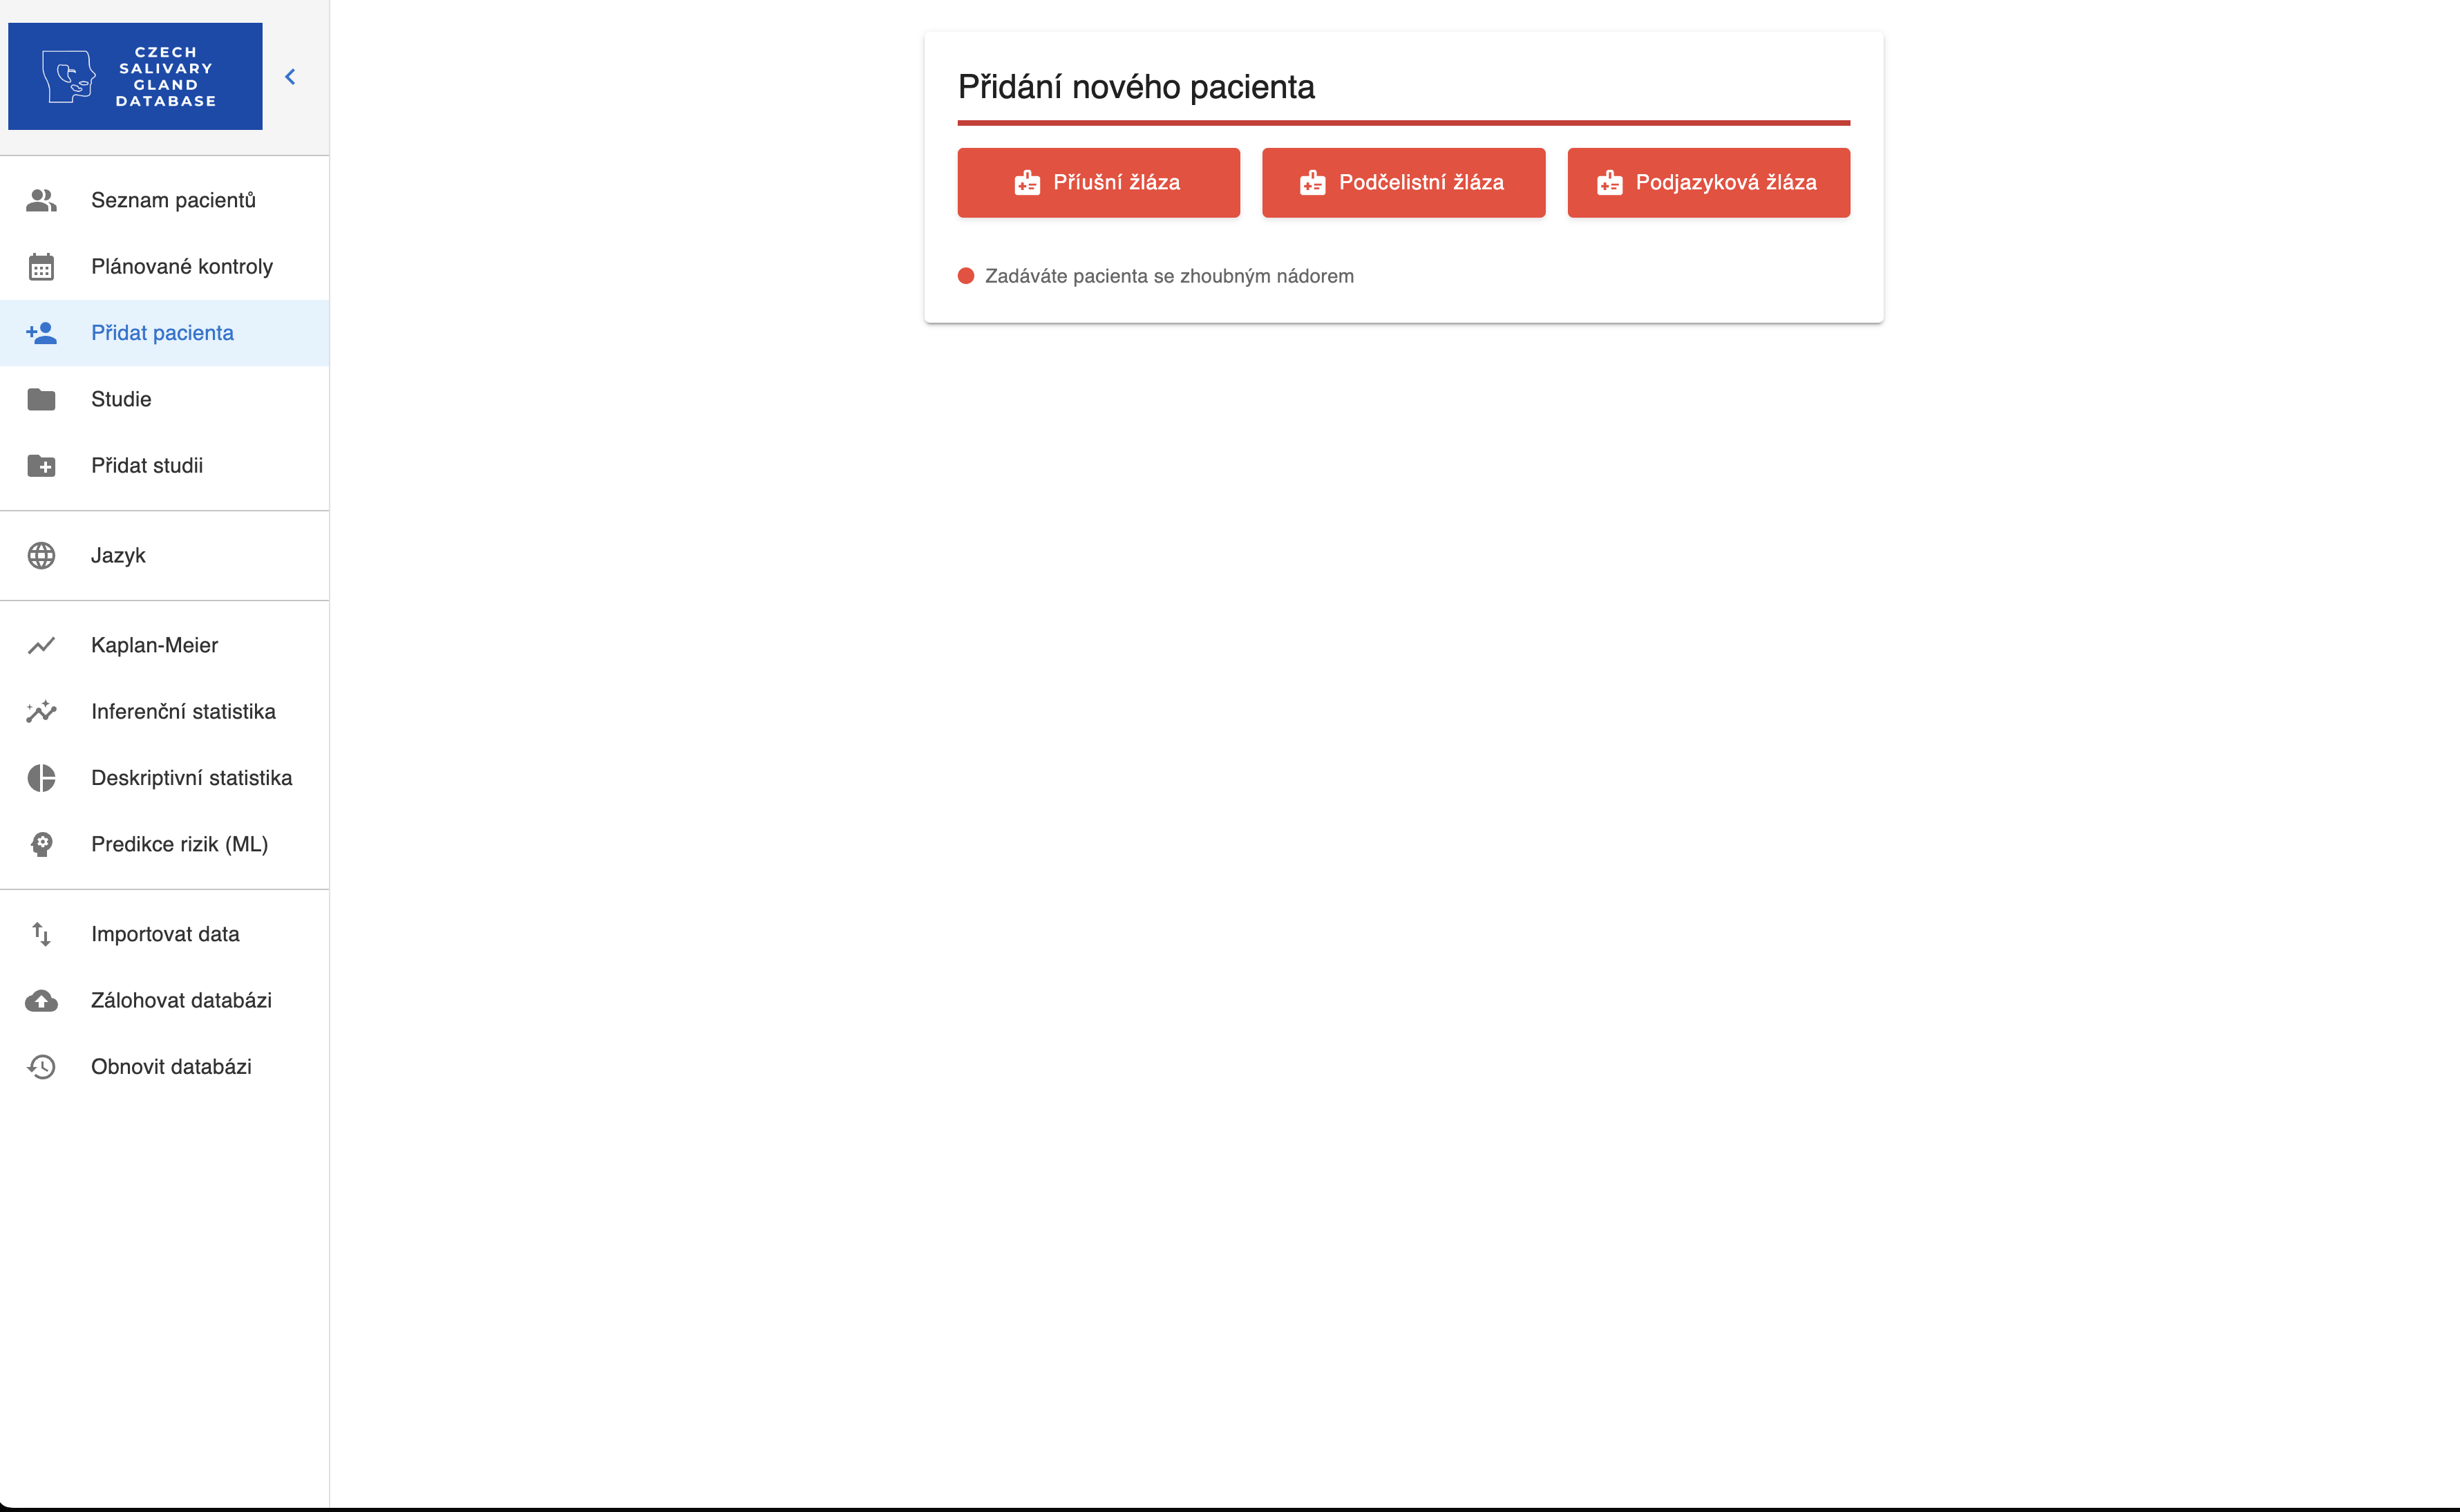
\includegraphics[width=0.85\textwidth]{img/pridani-pacienta/pridani_2.png}
        \caption{Krok 2: Výběr postižené slinné žlázy.}
        \label{fig:pridani-2}
    \end{figure}

    \item \textbf{Vyplnění anamnestických a personálních dat}:
    Na základě zvolené kombinace typu nádoru a žlázy se vygeneruje formulář (viz Obrázek~\ref{fig:pridani-3}). V~horní části formuláře je zobrazena štítková indikace zvolené kombinace (např. \texttt{Zhoubný nádor - Příušní žláza}).
    
    Formulář obsahuje strukturované sekce pro zadání podrobných údajů:
    \begin{itemize}
        \item \textbf{Základní informace}: Jméno, příjmení, identifikační kód pacienta, rodné číslo (bez lomítka) a věk v~době diagnózy.
        \item \textbf{Pohlaví pacienta}: Výběr pohlaví (Žena / Muž).
        \item \textbf{Demografické informace}: Kraj trvalého bydliště pacienta.
        \item \textbf{Klinická a histopatologická data}: Specifické informace o~diagnóze, chirurgickém výkonu, léčbě a sledování.
    \end{itemize}

    \begin{figure}[H]
        \centering
        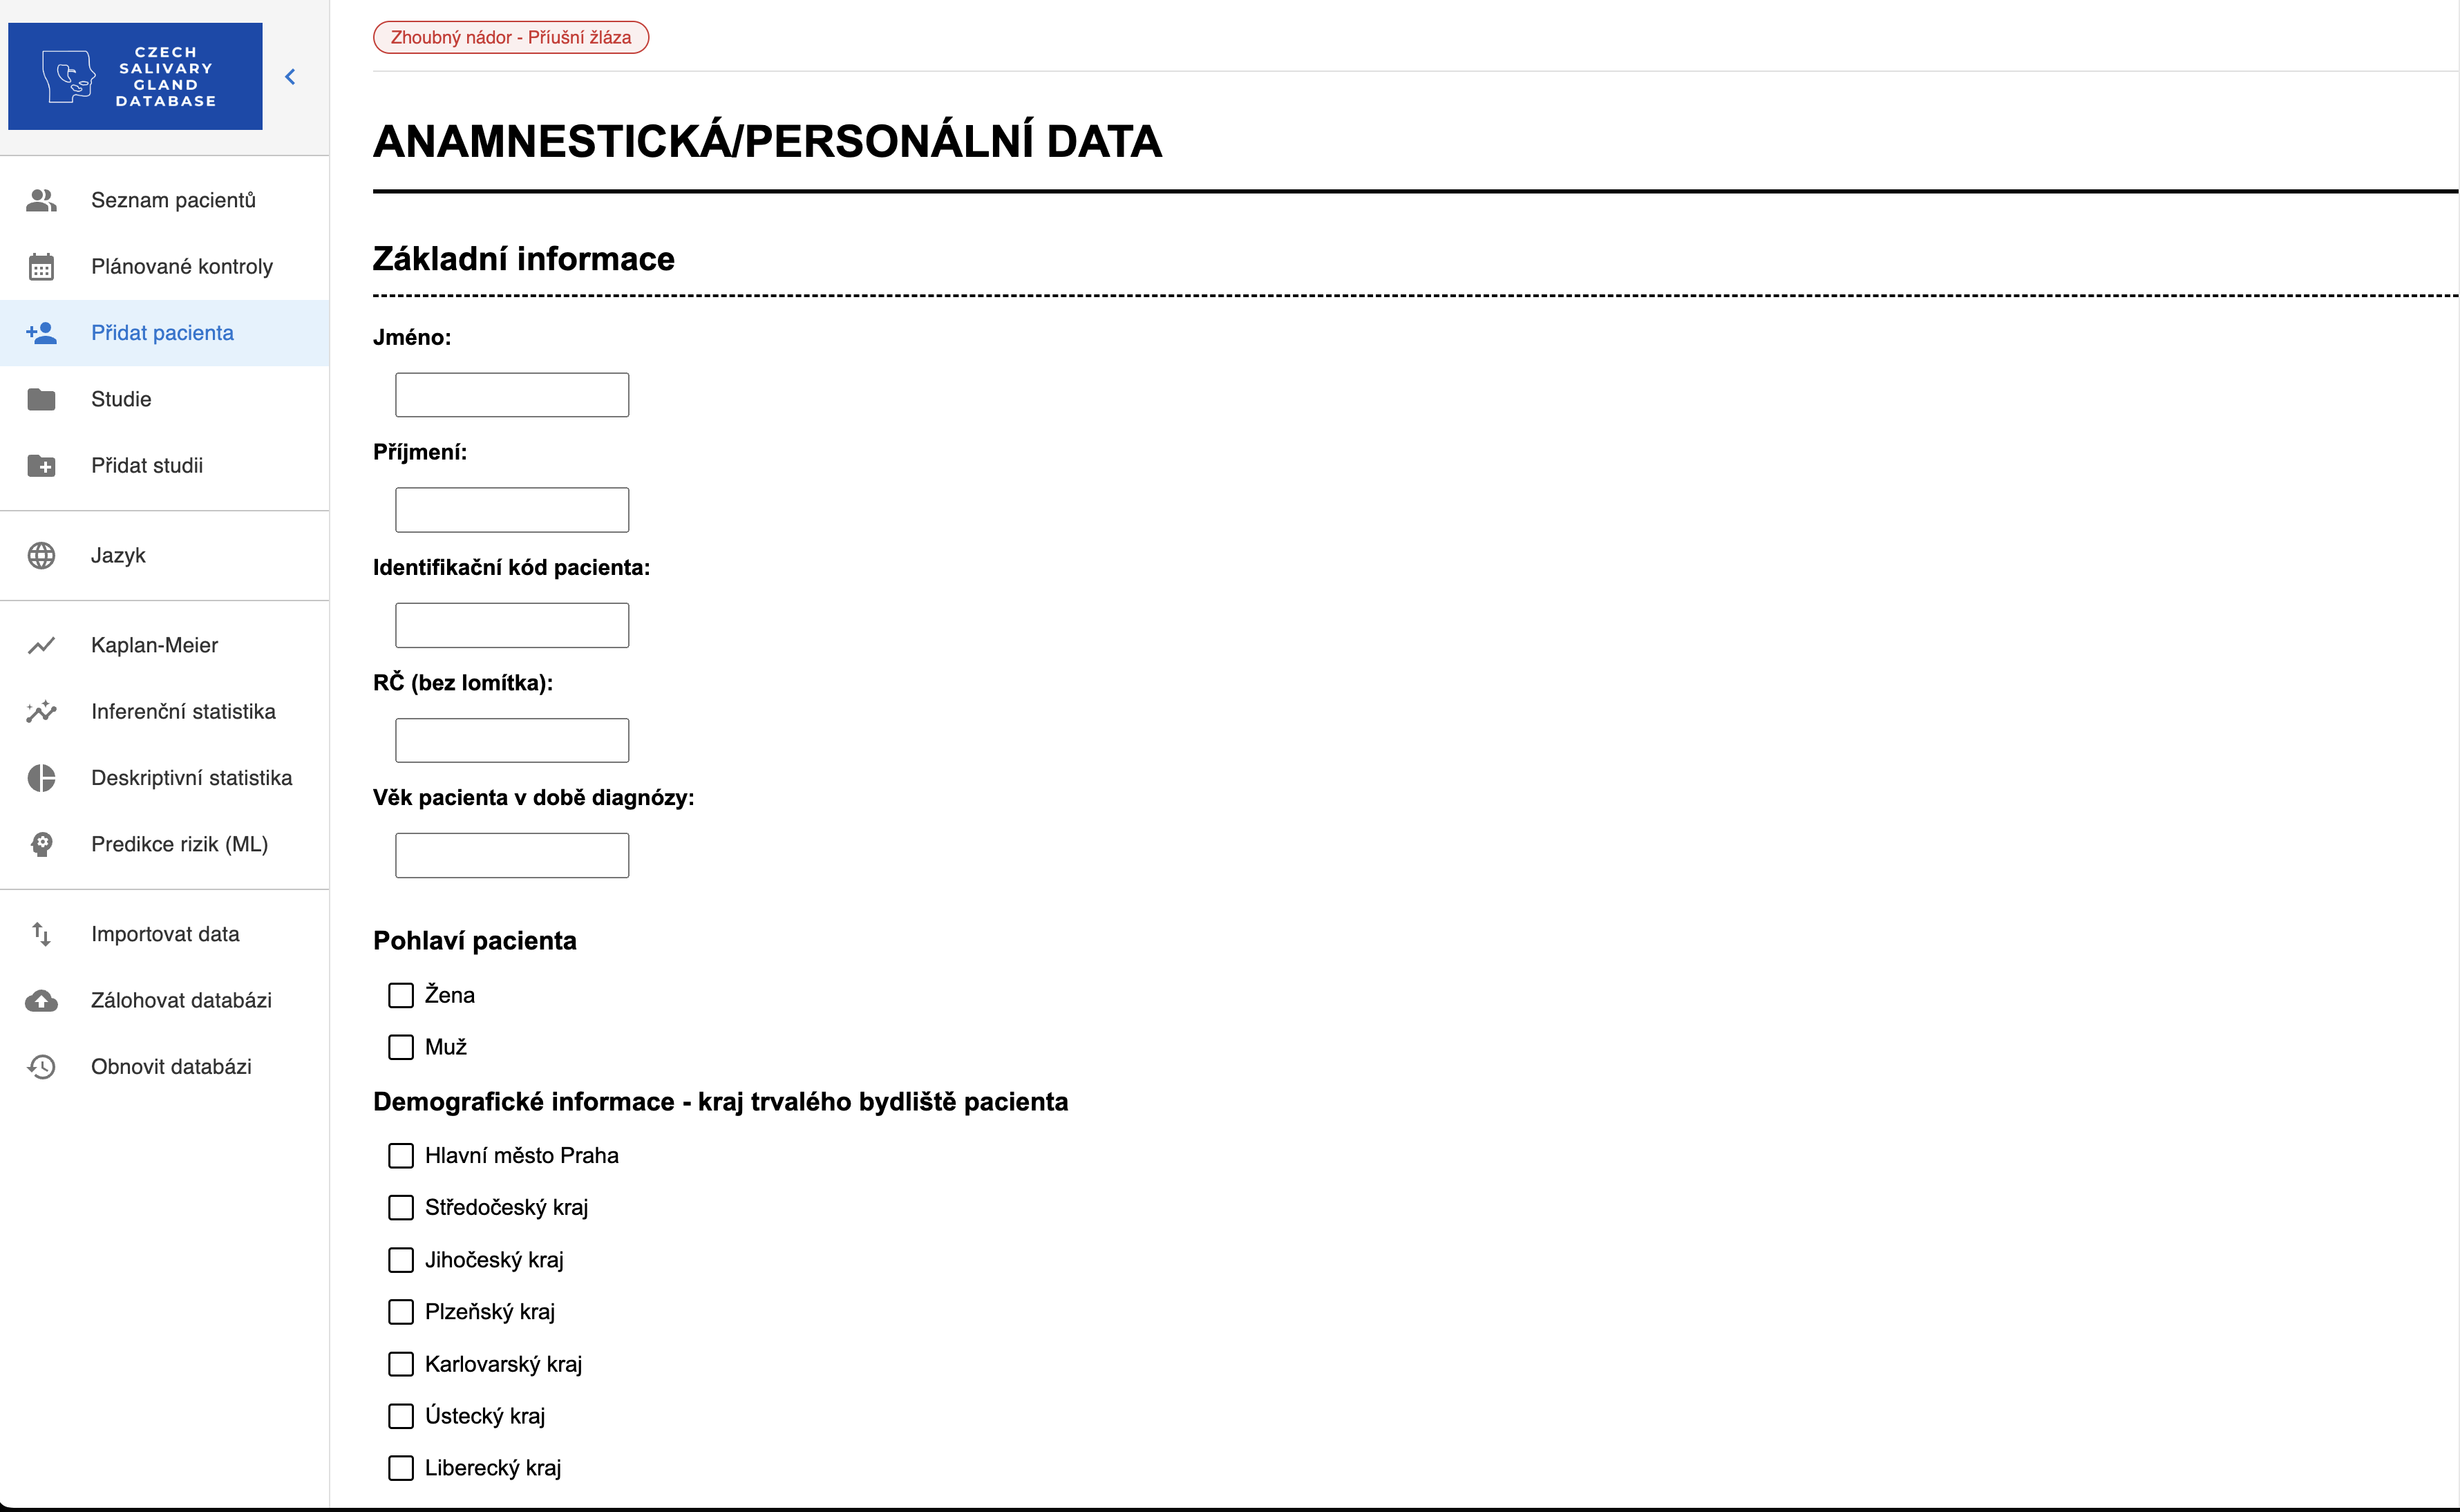
\includegraphics[width=0.85\textwidth]{img/pridani-pacienta/pridani_3.png}
        \caption{Krok 3: Vyplnění formuláře osobních a anamnestických dat.}
        \label{fig:pridani-3}
    \end{figure}

    Po dokončení vyplňování sjeďte na konec formuláře a klikněte na tlačítko \textbf{Přidat pacienta}. Pacient bude uložen do databáze a budete přesměrováni do části \textbf{Seznam pacientů} s~označeným nově přidaným záznamem.
\end{enumerate}

\subsection{Plánované kontroly}

Modul \textbf{Plánované kontroly} slouží k~přehledné časové evidenci a plánování nadcházejících lékařských kontrol u~pacientů.

\begin{enumerate}
    \item V~levém navigačním menu klikněte na záložku \textbf{Plánované kontroly}.
    \item V~horní části nastavte časový rozsah pomocí polí \textbf{Od} a \textbf{Do} pro výběr požadovaného období (viz Obrázek~\ref{fig:planovane-kontroly-1}).
    \item Na hlavní ploše se zobrazí kalendářové karty rozdělené podle jednotlivých dnů, ve kterých jsou uvedena jména pacientů s~plánovanou kontrolou.
    \item Chcete-li přehled kontrol vytisknout nebo uložit, klikněte v~pravém horním rohu na modré tlačítko \textbf{EXPORT PDF}. Aplikace vygeneruje přehledový dokument ve formátu PDF.

    \begin{figure}[H]
        \centering
        
\includegraphics[width=0.9\textwidth]{img/planovane-kontroly/planovane_kontroly_1.png}
        \caption{Přehled plánovaných kontrol s výběrem období a tlačítkem pro export do PDF.}
        \label{fig:planovane-kontroly-1}
    \end{figure}
\end{enumerate}

\subsection{Editace dat o pacientovi}

Pokud potřebujete upravit údaje již uloženého pacienta, postupujte následovně:

\begin{enumerate}
    \item \textbf{Výběr pacienta ze seznamu}:
    Přejděte do části \textbf{Seznam pacientů} (případně do konkrétní \textbf{Studie}, kde máte zobrazen seznam pacientů) a kliknutím v~seznamu vyberte pacienta, kterého chcete upravit (viz Obrázek~\ref{fig:edit-1}).
    
    V~pravé horní části pracovní plochy se nachází modré tlačítko s~ikonou tužky.

    \begin{figure}[H]
        \centering
        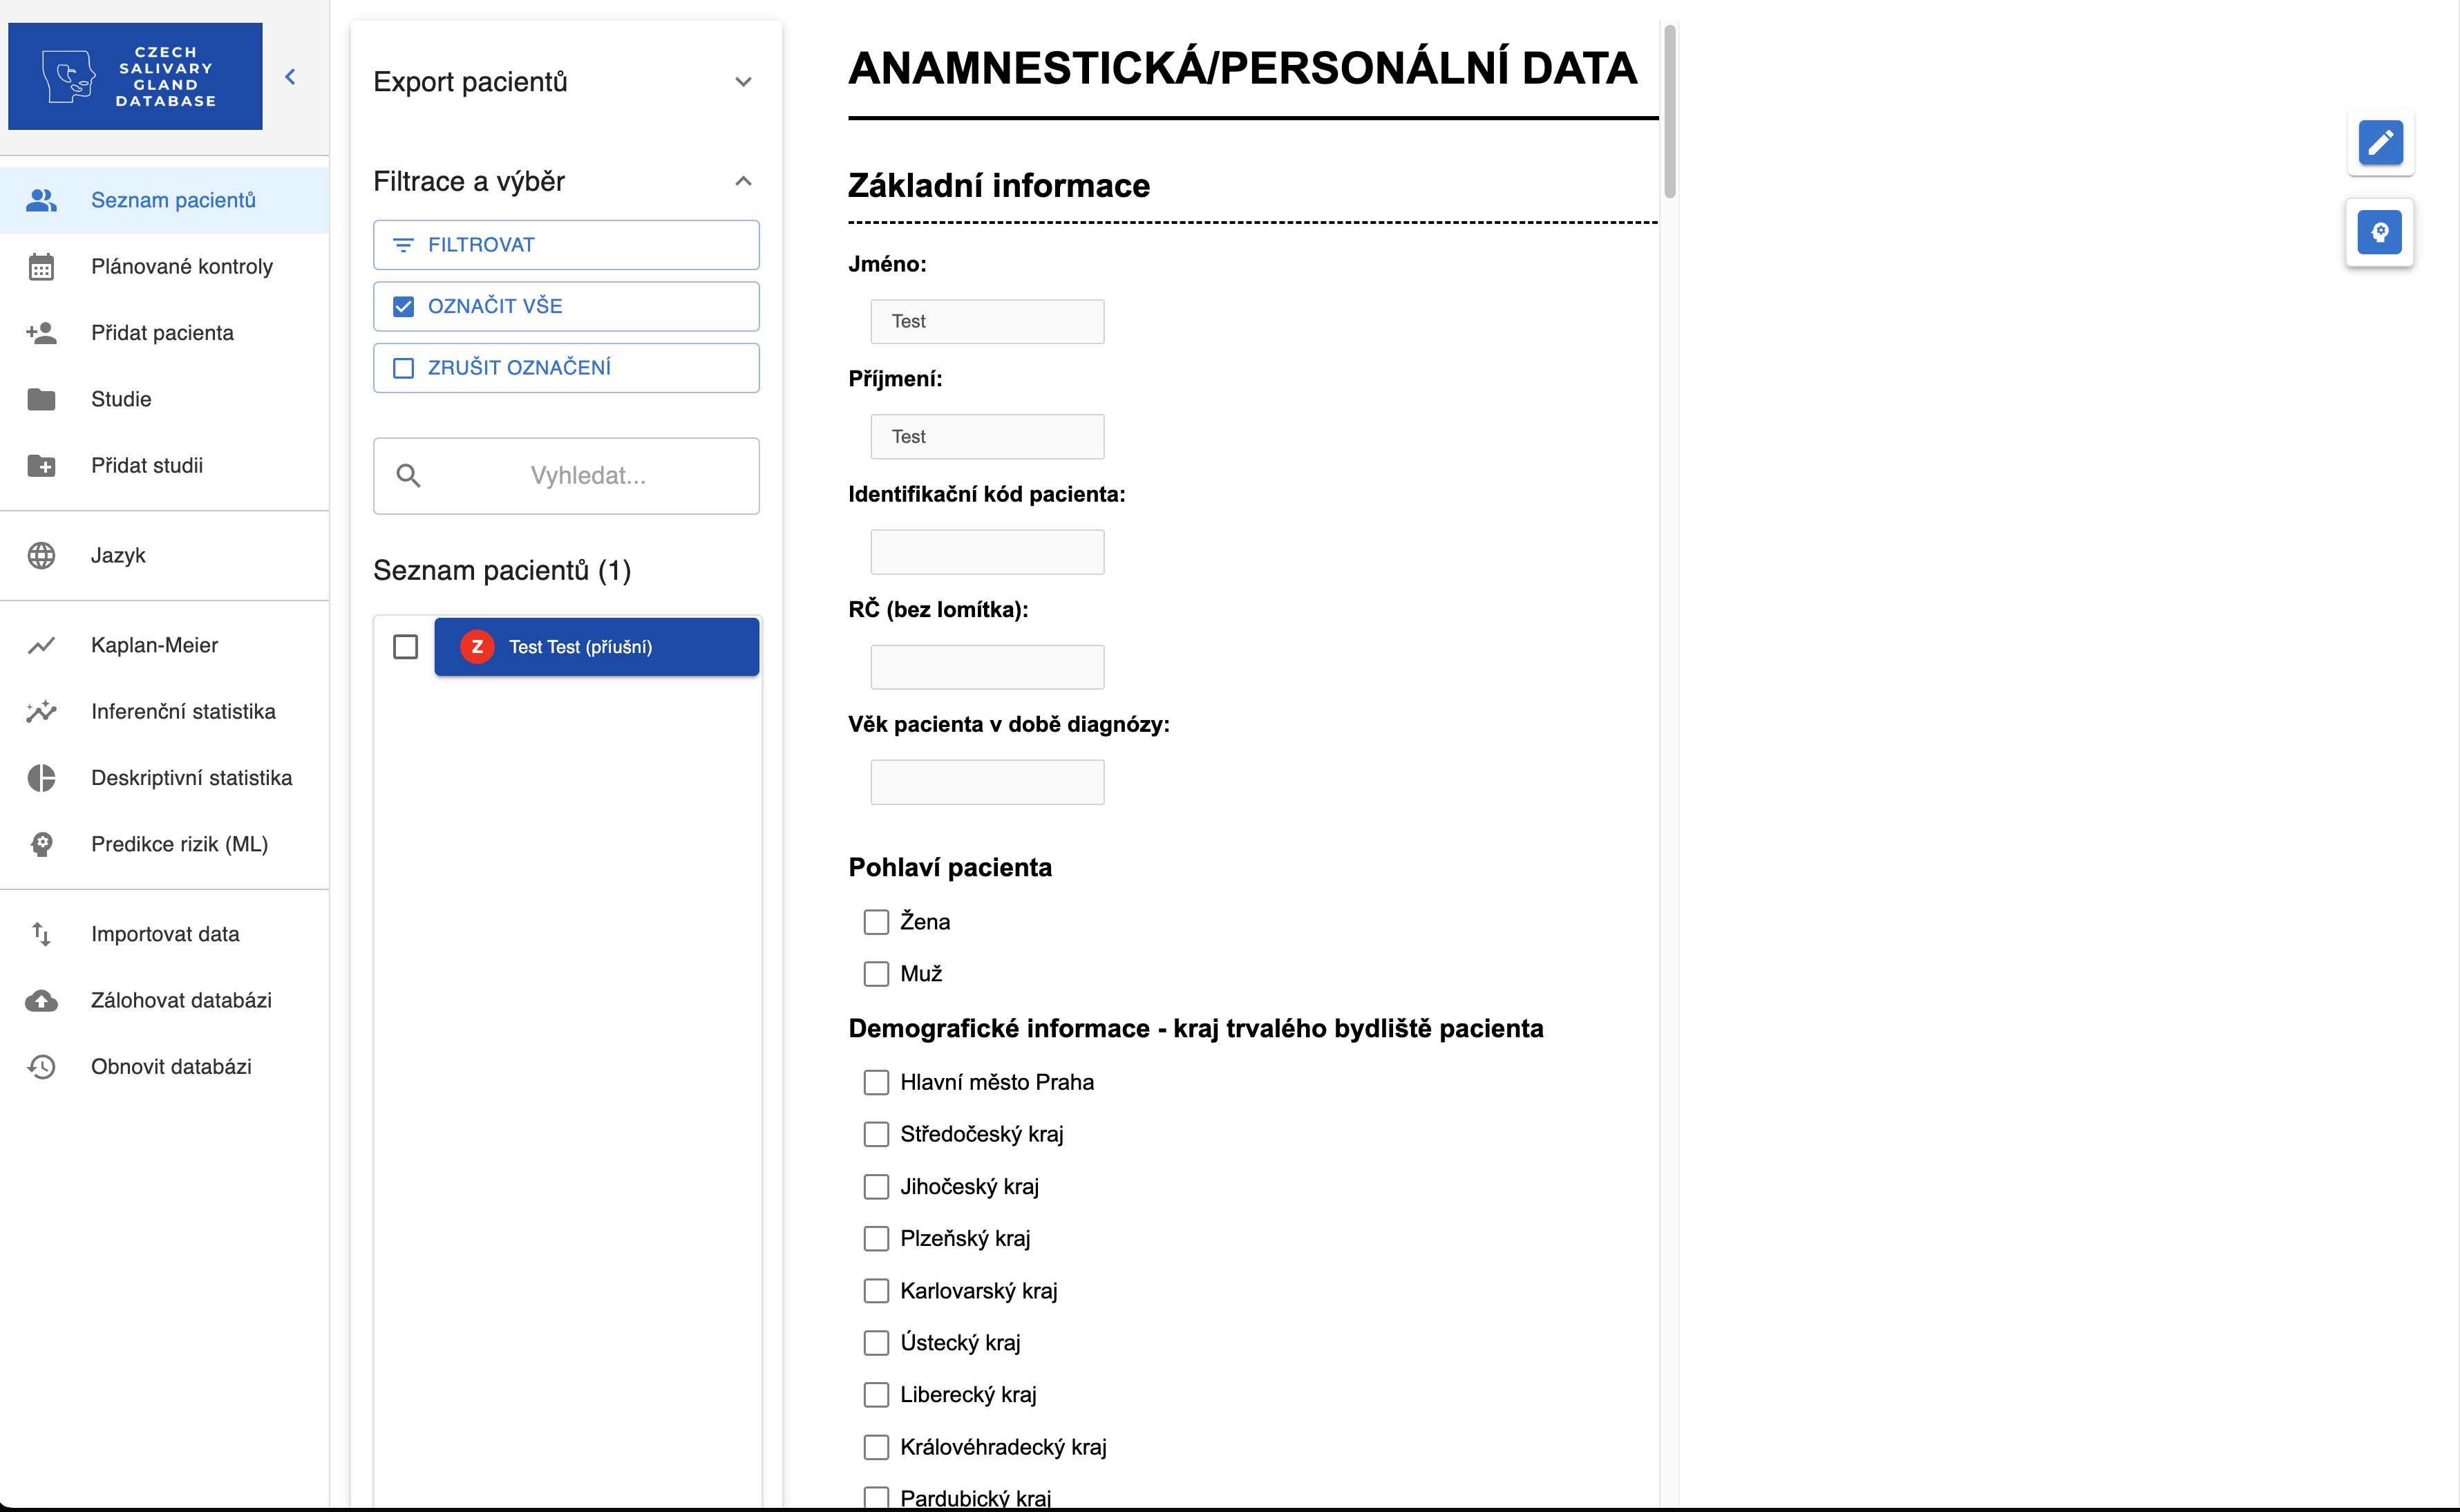
\includegraphics[width=0.85\textwidth]{img/editace-pacienta/edit_1.png}
        \caption{Karta pacienta s~tlačítkem pro vyvolání akcí v~pravém horním rohu.}
        \label{fig:edit-1}
    \end{figure}

    \item \textbf{Aktivace režimu úprav}:
    Kliknutím na modré tlačítko se v~horní části rozbalí nabídka akcí. Pro zahájení úprav klikněte na možnost \textbf{EDITOVAT} (viz Obrázek~\ref{fig:edit-2}).

    \begin{figure}[H]
        \centering
        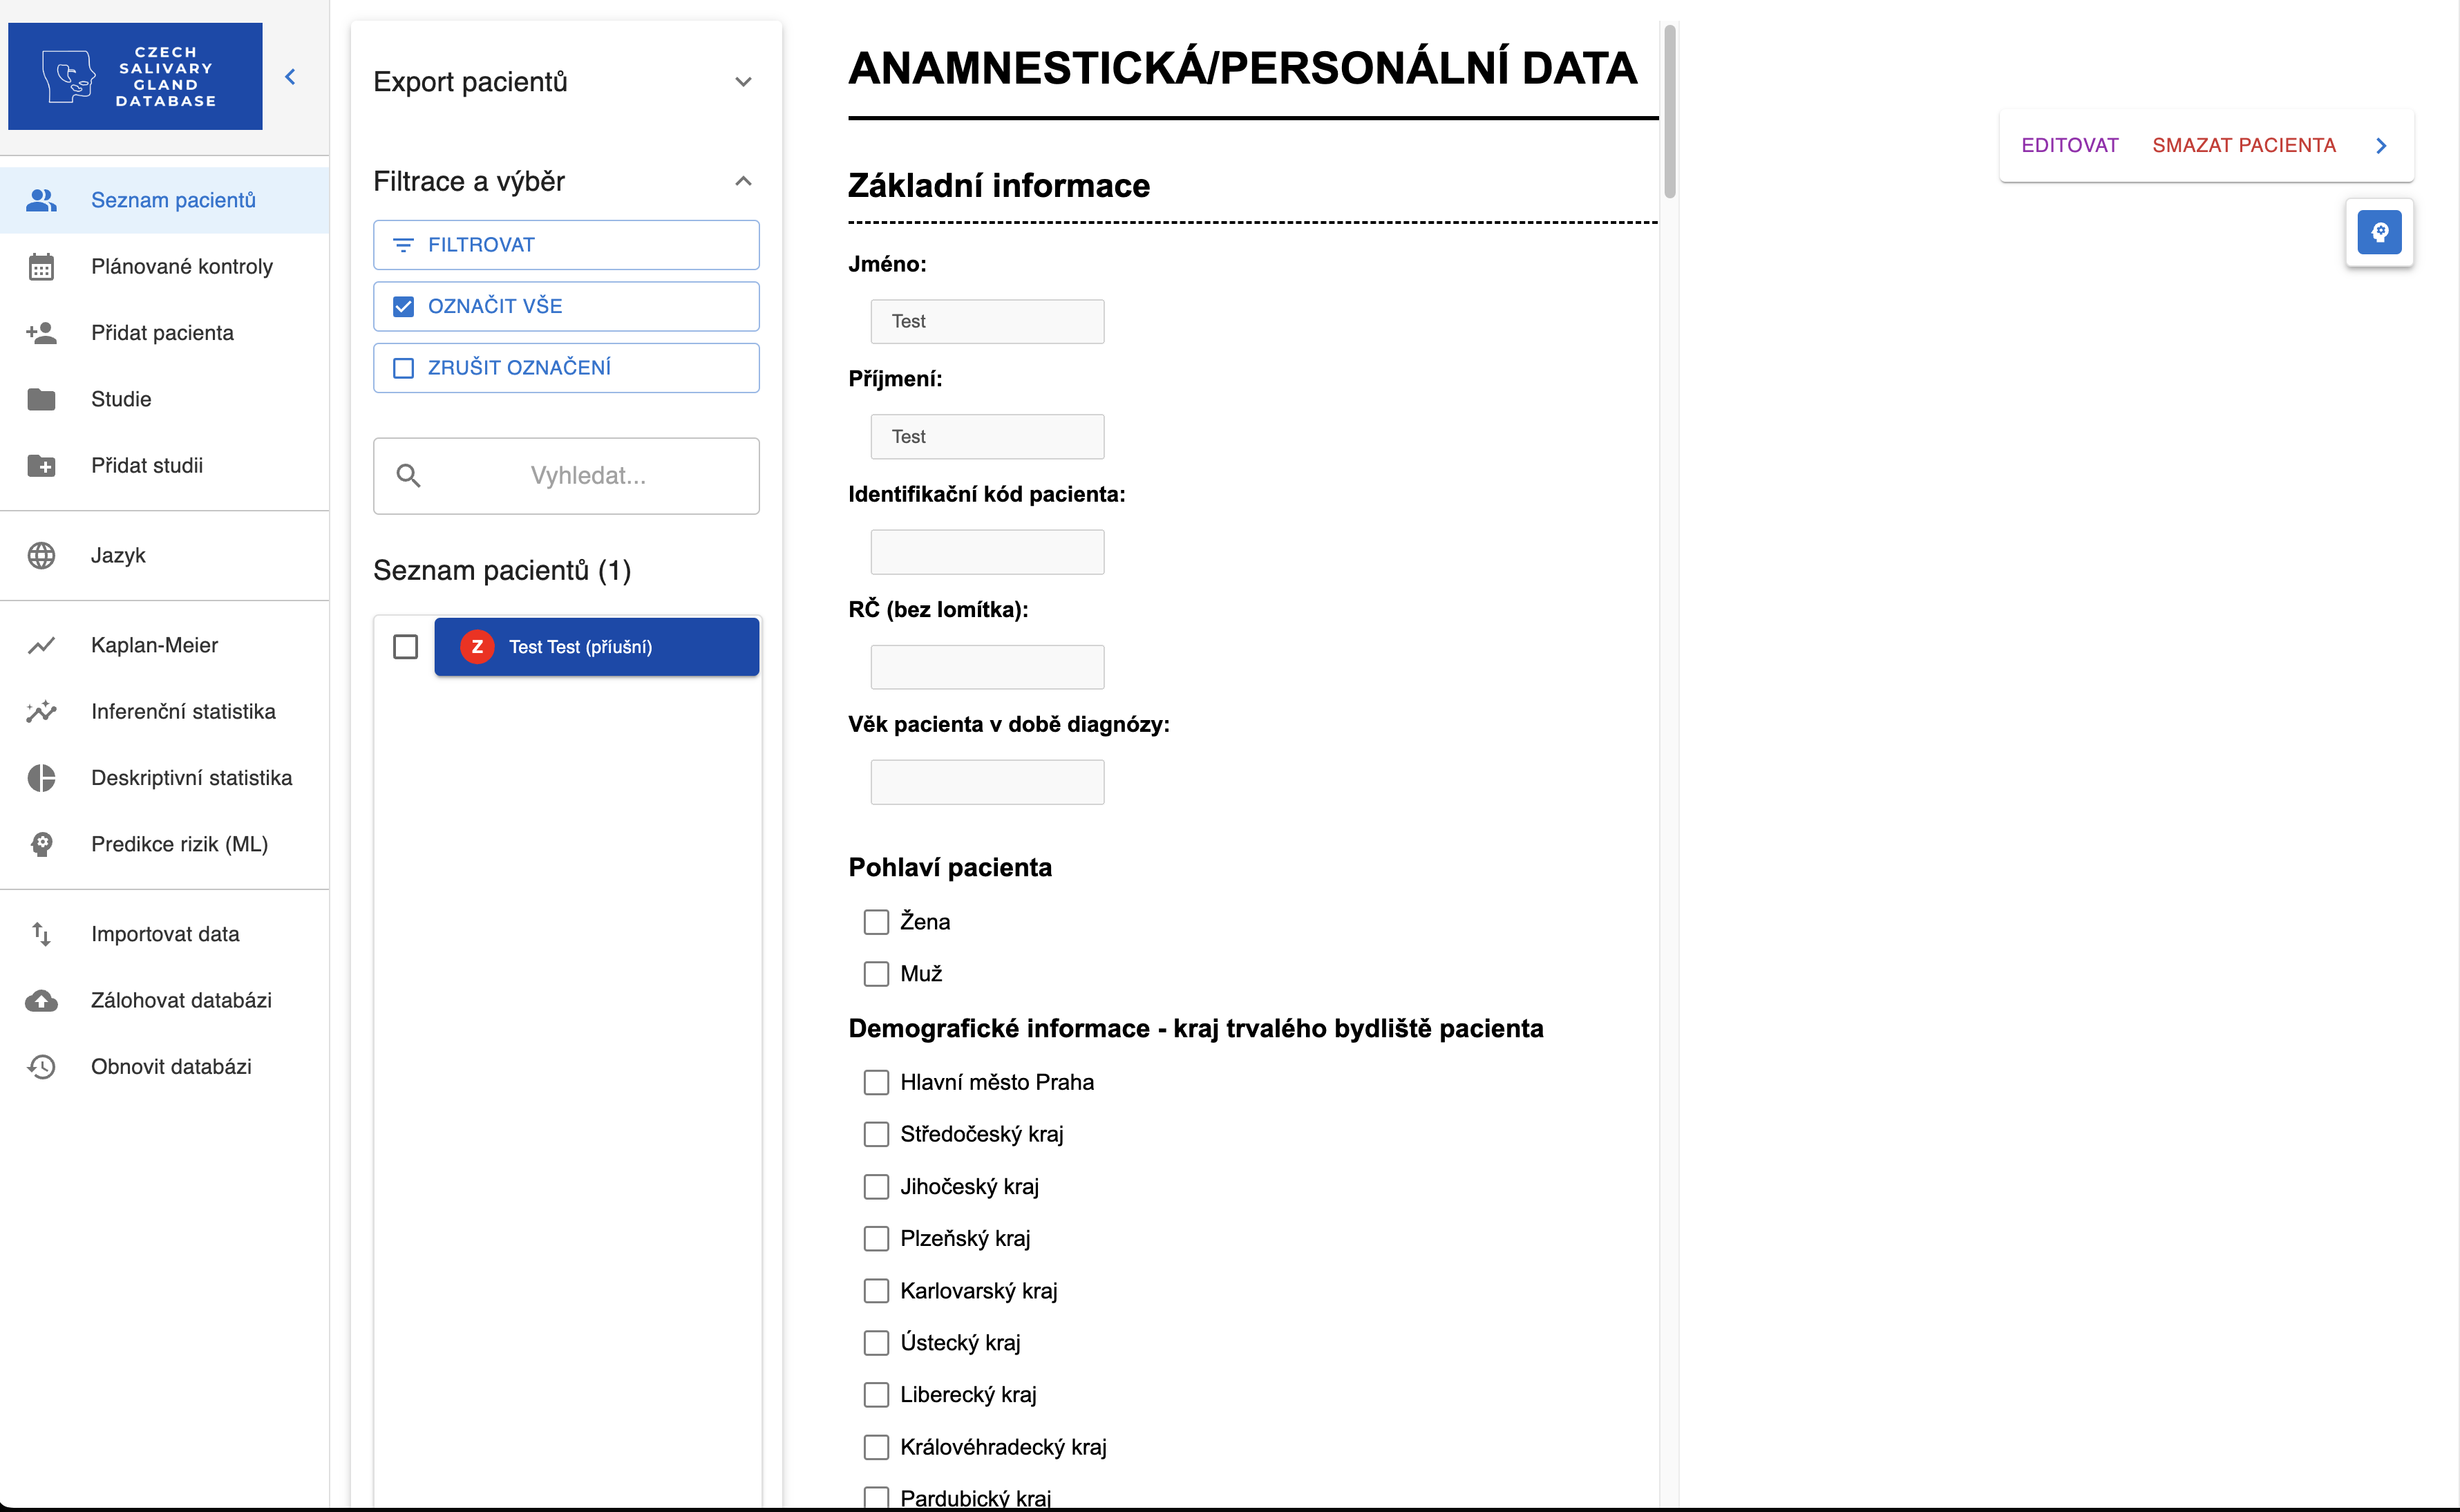
\includegraphics[width=0.85\textwidth]{img/editace-pacienta/edit_2.png}
        \caption{Rozbalená nabídka akcí s~tlačítkem EDITOVAT.}
        \label{fig:edit-2}
    \end{figure}

    \item \textbf{Úprava údajů a uložení nebo zrušení změn}:
    Po stisknutí tlačítka \textbf{EDITOVAT} se formulář zpřístupní pro úpravy a v~pravé horní liště se objeví ovládací tlačítka (viz Obrázek~\ref{fig:edit-3}):
    \begin{itemize}
        \item \textbf{ULOŽIT ZMĚNY} -- uložení všech provedených úprav do databáze.
        \item \textbf{ZRUŠIT EDITACI} -- storno provedených změn a návrat k~původním datům.
        \item \textbf{SMAZAT PACIENTA} -- možnost trvalého odstranění pacienta z~databáze.
    \end{itemize}

    \begin{figure}[H]
        \centering
        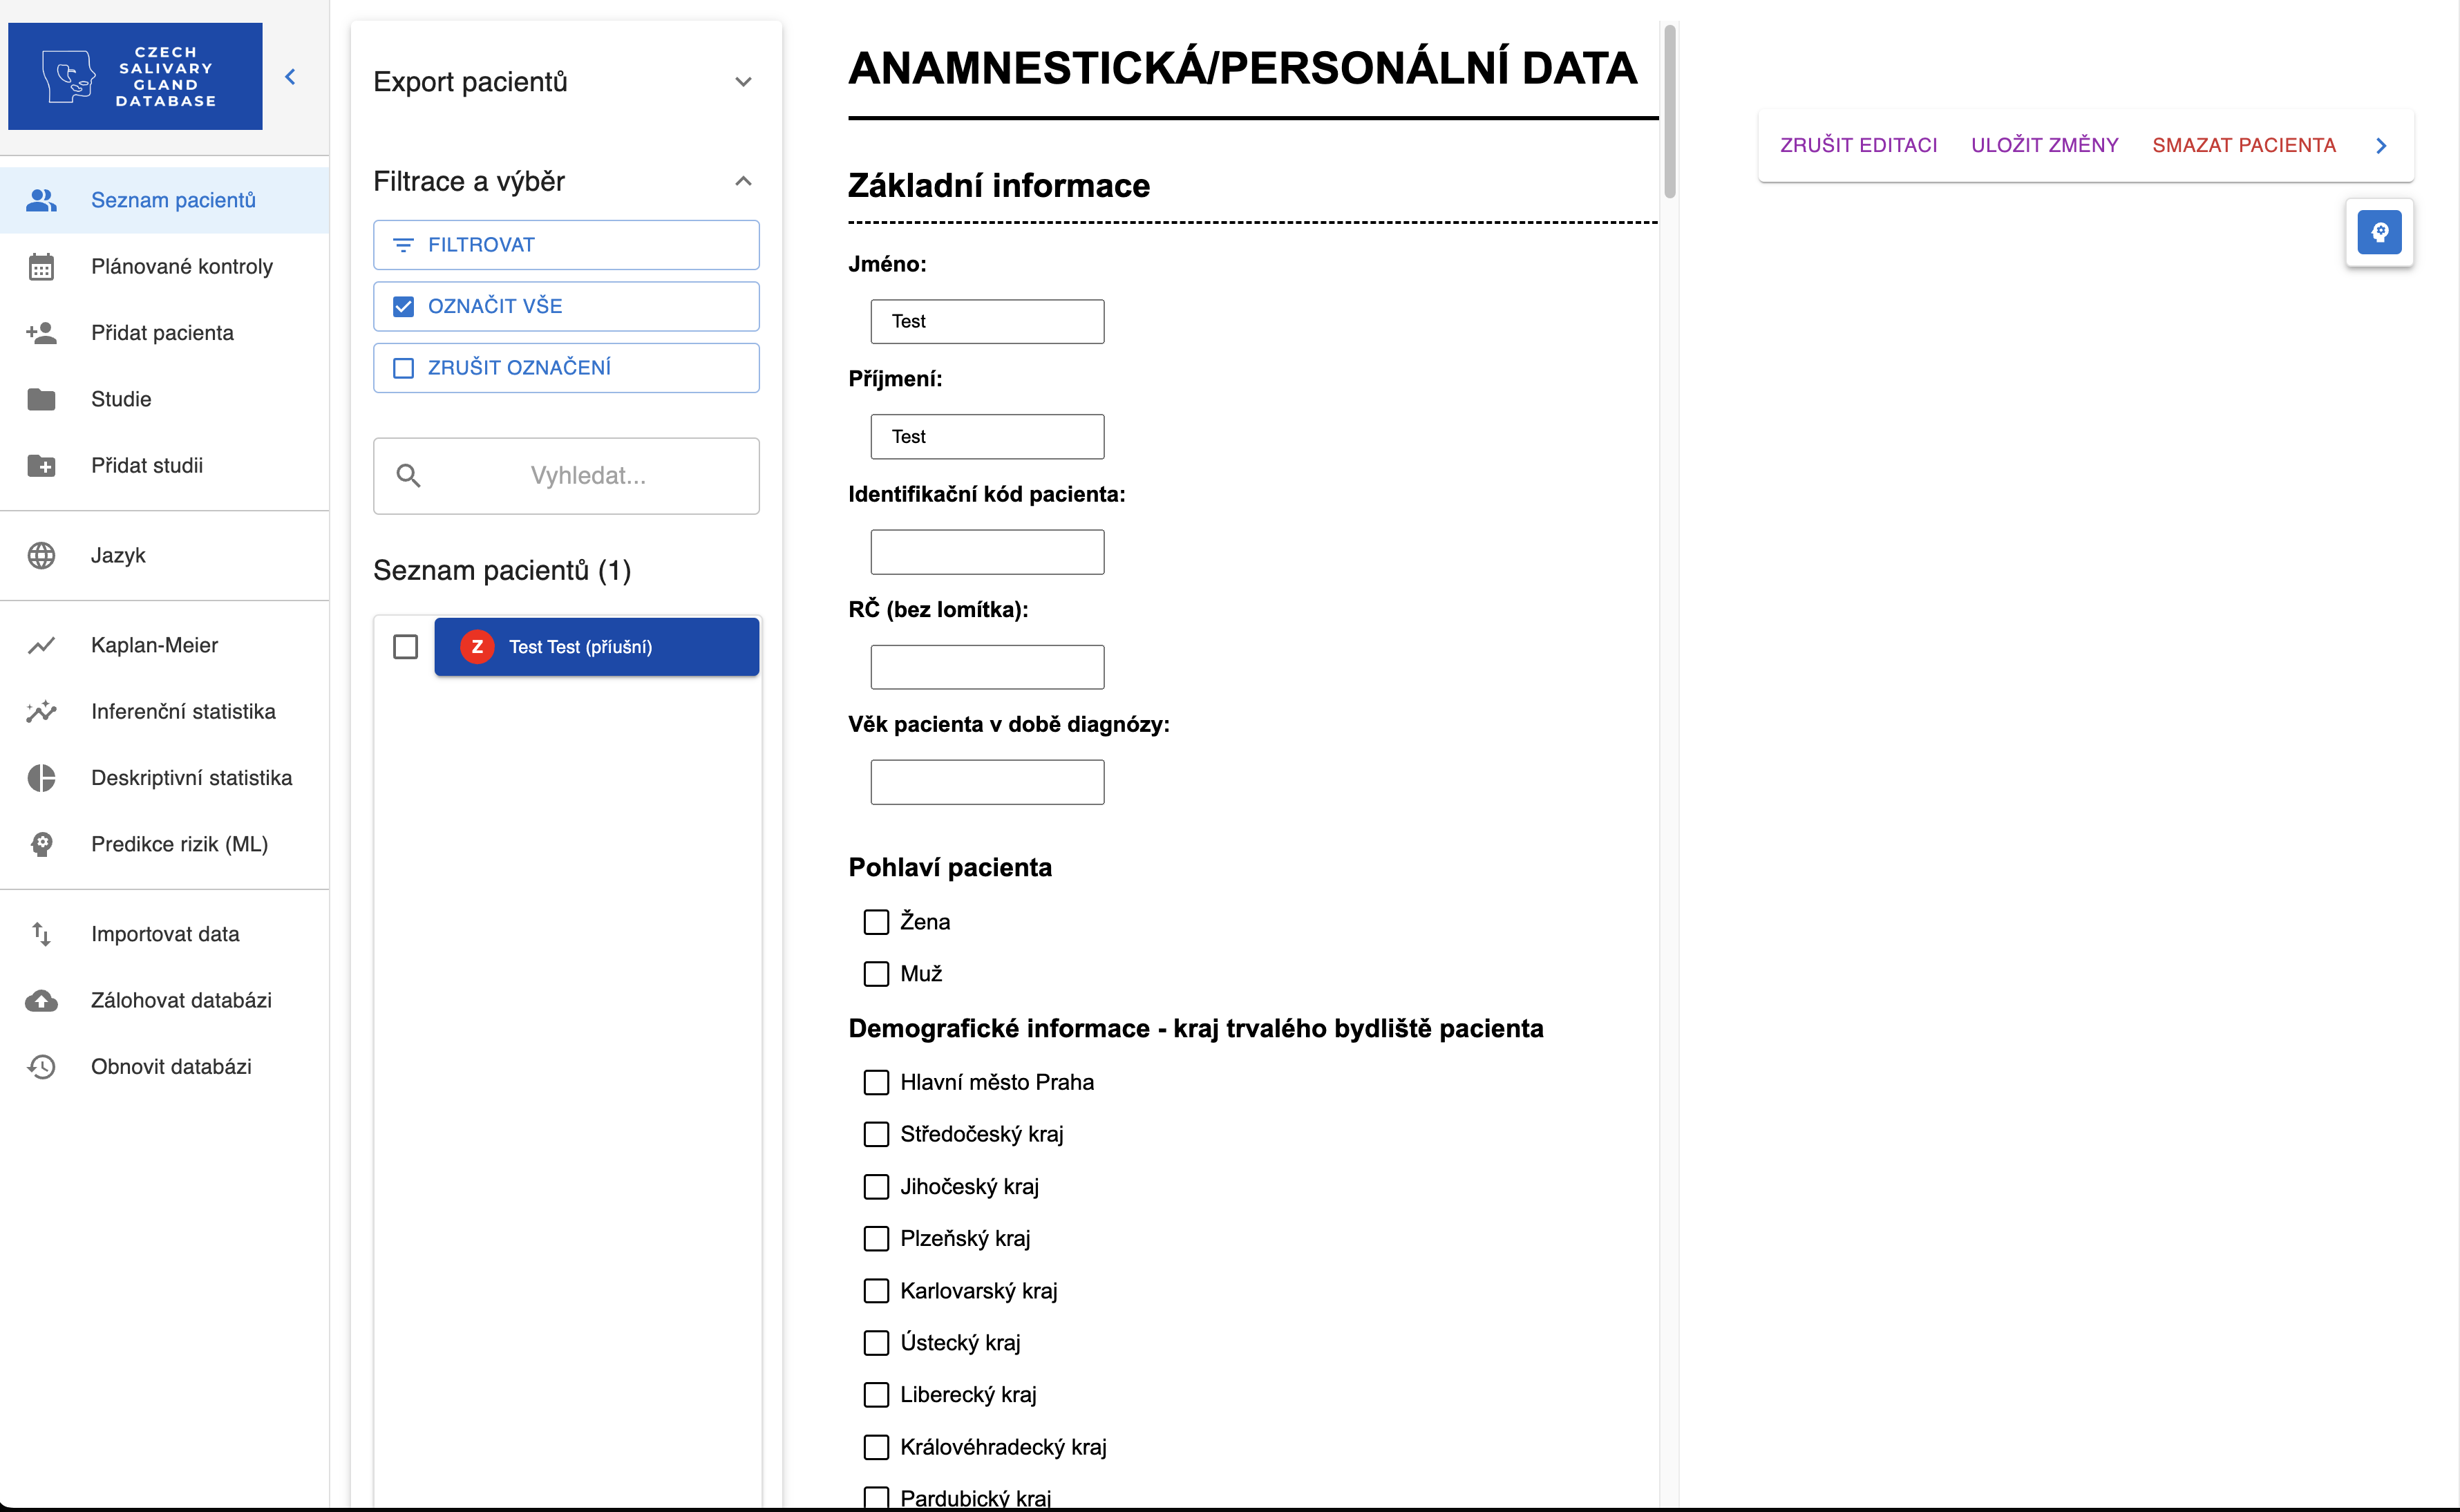
\includegraphics[width=0.85\textwidth]{img/editace-pacienta/edit_3.png}
        \caption{Režim editace s~ovládacími tlačítky ULOŽIT ZMĚNY a ZRUŠIT EDITACI.}
        \label{fig:edit-3}
    \end{figure}
\end{enumerate}

\subsection{Vyhledávání a filtrace v seznamu pacientů}

V~aplikaci \texttt{csgdb} lze v~seznamu pacientů (v~záložkách \textbf{Seznam pacientů} i \textbf{Studie}) snadno vyhledávat a filtrovat záznamy podle nejrůznějších klinických a demografických kritérií.

\subsubsection{Rychlé vyhledávání}
Pro rychlé nalezení konkrétního pacienta slouží vstupní pole \textbf{Vyhledat...} umístěné v~horní části středního panelu v~sekci \textit{Filtrace a výběr} (viz Obrázek~\ref{fig:vyhledavani-1}).

\begin{figure}[H]
    \centering
    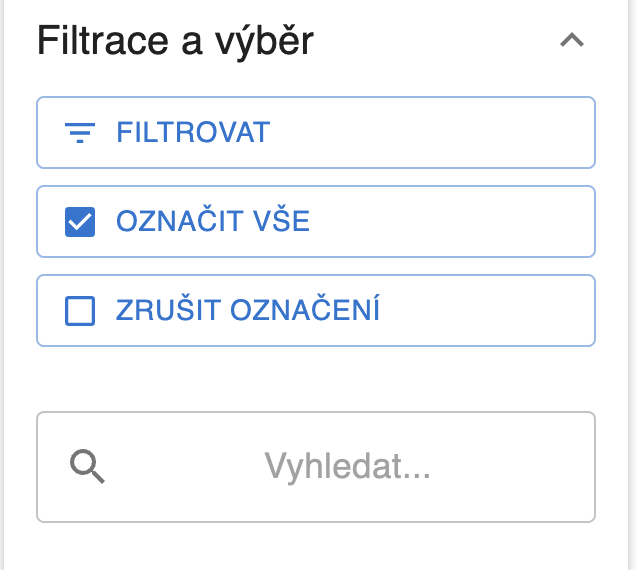
\includegraphics[width=0.45\textwidth]{img/vyhledavani-a-filtrace/vyhledavani_a_filtrace_1.png}
    \caption{Sekce Filtrace a výběr s~vyhledávacím polem a ovládacími tlačítky.}
    \label{fig:vyhledavani-1}
\end{figure}

Vyhledávání probíhá v~reálném čase během psaní a vyhledává shody podle:
\begin{itemize}
    \item \textbf{jména a příjmení} pacienta,
    \item \textbf{rodného čísla} (případně identifikačního kódu pacienta).
\end{itemize}

\subsubsection{Pokročilá filtrace pacientů}
Pro podrobné přeshraniční či klinické filtrování klikněte na tlačítko \textbf{FILTROVAT}. Zobrazí se postranní dialogové okno \textbf{Filtrační menu} (viz Obrázek~\ref{fig:vyhledavani-2}).

\begin{figure}[H]
    \centering
    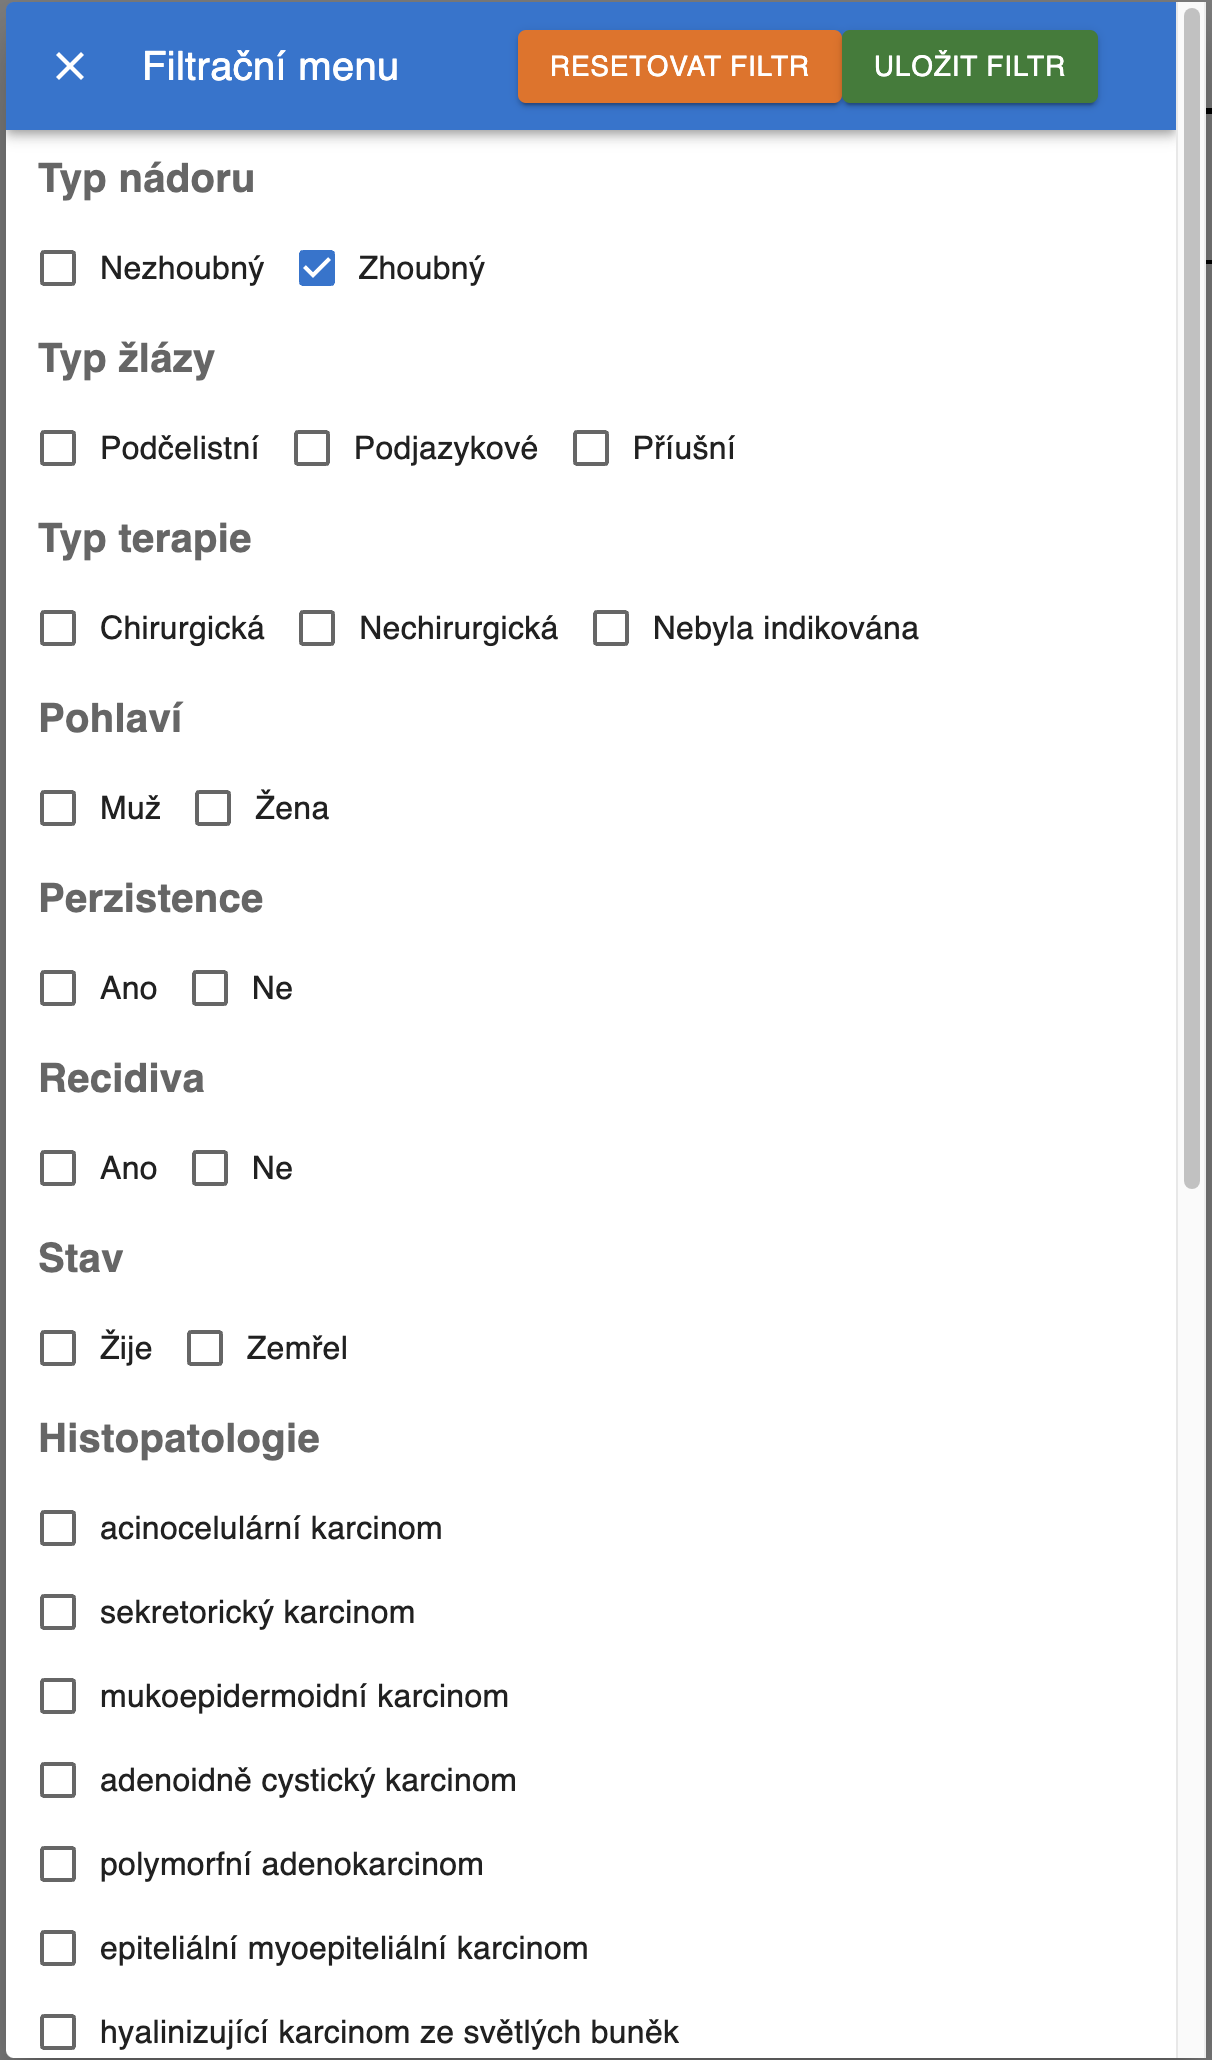
\includegraphics[width=0.55\textwidth]{img/vyhledavani-a-filtrace/vyhledavani_a_filtrace_2.png}
    \caption{Filtrační menu pro nastavení podrobných kritérií výběru.}
    \label{fig:vyhledavani-2}
\end{figure}

Filtrační menu umožňuje nastavit libovolnou kombinaci vybraných parametrů.

\textbf{Aplikace a zrušení filtru}:
\begin{itemize}
    \item Po nastavení požadovaných kritérií klikněte na zelené tlačítko \textbf{ULOŽIT FILTR}. Seznam pacientů se okamžitě přefiltruje podle zadaných parametrů.
    \item Chcete-li aktivní filtr zrušit a zobrazit opět všechny pacienty, otevřete filtrační menu a klikněte na oranžové tlačítko \textbf{RESETOVAT FILTR}.
\end{itemize}

\subsection{Export pacientů}

Aplikace \texttt{csgdb} umožňuje exportovat vybrané záznamy pacientů do formátu Microsoft Excel (\texttt{.xls}) pro další zpracování či výzkum. Export lze provést ze záložky \textbf{Seznam pacientů} i z~detailu konkrétní \textbf{Studie}.

\subsubsection{Postup při exportu dat}

\begin{enumerate}
    \item \textbf{Výběr pacientů pro export}:
    V~seznamu pacientů označte záznamy, které chcete exportovat:
    \begin{itemize}
        \item zaškrtnutím políčka (checkboxu) u~jednotlivých pacientů, nebo
        \item kliknutím na tlačítko \textbf{OZNAČIT VŠE} v~sekci \textit{Filtrace a výběr} pro označení všech zobrazených pacientů.
    \end{itemize}

    \item \textbf{Volba typu exportu}:
    Rozbalte panel \textbf{Export pacientů} umístěný v~horní části středního panelu (viz Obrázek~\ref{fig:export-1}). K~dispozici máte dvě možnosti:
    \begin{itemize}
        \item \textbf{Exportovat} (světle zelené tlačítko s~šipkami) -- provede standardní export všech zadaných údajů o~pacientech včetně osobních identifikačních dat.
        \item \textbf{Exportovat anonymizovaně} (tmavě zelené tlačítko se štítem) -- provede anonymizovaný export, ze kterého jsou odstraněny osobní identifikátory (jméno, příjmení, rodné číslo), což je ideální pro vědecké publikace a sdílení dat s~třetími stranami.
    \end{itemize}

    \begin{figure}[H]
        \centering
        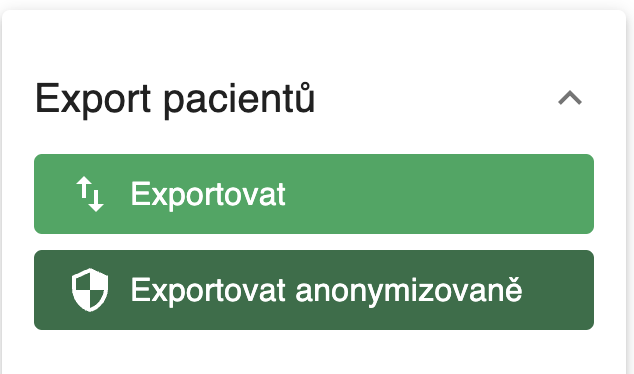
\includegraphics[width=0.45\textwidth]{img/export/export_1.png}
        \caption{Možnosti v~sekci Export pacientů (standardní a anonymizovaný export).}
        \label{fig:export-1}
    \end{figure}

    \item \textbf{Uložení souborů}:
    Po kliknutí na zvolené tlačítko exportu se zobrazí systémové dialogové okno vašho operačního systému, ve kterém zvolíte cílový adresář pro uložení.

    \item \textbf{Struktura vygenerovaných souborů}:
    Data jsou následně uložena ve formátu \texttt{.xls}. Pro každý typ slinné žlázy (příušní, podčelistní, podjazyková), ve které se nacházejí vybraní pacienti, je automaticky vytvořen samostatný Excel soubor.
\end{enumerate}

\section{Práce se studiemi}

Modul studií umožňuje seskupovat vybrané pacienty do samostatných výzkumných či klinických souborů (studií), sledovat je odděleně a provádět nad nimi specifické analýzy a exporty.

\subsection{Vytvoření nové studie}
\label{sec:vytvoreni-studie}

Postup vytvoření nové studie probíhá v~následujících krocích:

\begin{enumerate}
    \item \textbf{Přechod do nabídky vytváření studie}:
    V~levém navigačním menu klikněte na položku \textbf{Přidat studii}. Zobrazí se obrazovka s~výběrem typu studie podle zasažené žlázy (viz Obrázek~\ref{fig:pridani-studie-1}):
    \begin{itemize}
        \item \textbf{NOVÁ STUDIE PŘÍUŠNÍCH ŽLÁZ} -- studie určená pouze pro pacienty s~onemocněním příušní žlázy,
        \item \textbf{NOVÁ STUDIE PODČELISTNÍCH ŽLÁZ} -- studie pro pacienty s~onemocněním podčelistní žlázy,
        \item \textbf{NOVÁ STUDIE PODJAZYKOVÝCH ŽLÁZ} -- studie pro pacienty s~onemocněním podjazykové žlázy,
        \item \textbf{NOVÁ STUDIE SPECIÁLNÍ STUDIE} -- speciální studie, do které lze zařadit pacienty napříč všemi typy žláz.
    \end{itemize}

    \begin{figure}[H]
        \centering
        
\includegraphics[width=0.85\textwidth]{img/pridani-studie/pridani_1.png}
        \caption{Krok 1: Výběr typu vytvářené studie podle zasažené žlázy.}
        \label{fig:pridani-studie-1}
    \end{figure}

    \item \textbf{Zadání názvu studie a výběr pacientů}:
    Po výběru typu studie se v~prostředním panelu zobrazí rozhraní pro nastavení studie a seznam pacientů odpovídajících zvolené kategorii (viz Obrázek~\ref{fig:pridani-studie-2}):
    \begin{itemize}
        \item Do pole \textbf{Název studie} zadejte požadovaný název nové studie.
        \item V~seznamu pacientů označte zaškrtnutím políčka (checkboxu) ty pacienty, které chcete do studie zařadit. Můžete využít také tlačítka pro rychlou filtraci nebo tlačítko \textbf{OZNAČIT VŠE}.
    \end{itemize}

    \begin{figure}[H]
        \centering
        
\includegraphics[width=0.85\textwidth]{img/pridani-studie/pridani_2.png}
        \caption{Krok 2: Zadání názvu studie a zařazení pacientů z~nabídky.}
        \label{fig:pridani-studie-2}
    \end{figure}

    \item \textbf{Dokončení vytvoření studie}:
    Stiskněte tlačítko \textbf{VYTVOŘIT NOVOU STUDII}. Aplikace studii vytvoří, uloží do databáze a automaticky vás přesměruje do záložky \textbf{Studie}, kde bude vaše nová studie vybrána a připravena k~práci.
\end{enumerate}

\subsection{Editace a mazání studií}

Správu existujících studií (změnu jejich názvu nebo trvalé odstranění) lze provádět v~záložce \textbf{Studie}.

\subsubsection{Změna názvu studie}

\begin{enumerate}
    \item Přejděte do záložky \textbf{Studie} v~levém navigačním menu.
    \item V~prostředním panelu vyhledejte studii, jejíž název chcete změnit. Vedle názvu studie se nacházejí dvě ikony -- ikona tužky a ikona popelnice (viz Obrázek~\ref{fig:editace-studie-1}).

    \begin{figure}[H]
        \centering
        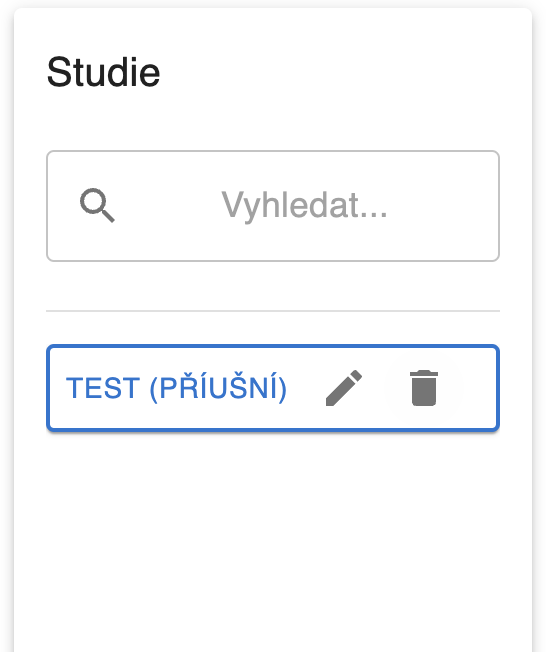
\includegraphics[width=0.45\textwidth]{img/editace-studie/editace_1.png}
        \caption{Seznam studií s tlačítky pro úpravu (tužka) a mazání (popelnice).}
        \label{fig:editace-studie-1}
    \end{figure}

    \item Klikněte na ikonu \textbf{tužky}. Název studie se změní na textové pole a objeví se ikona pro uložení (fajfka) a ikona pro zrušení (křížek) (viz Obrázek~\ref{fig:editace-studie-2}).

    \begin{figure}[H]
        \centering
        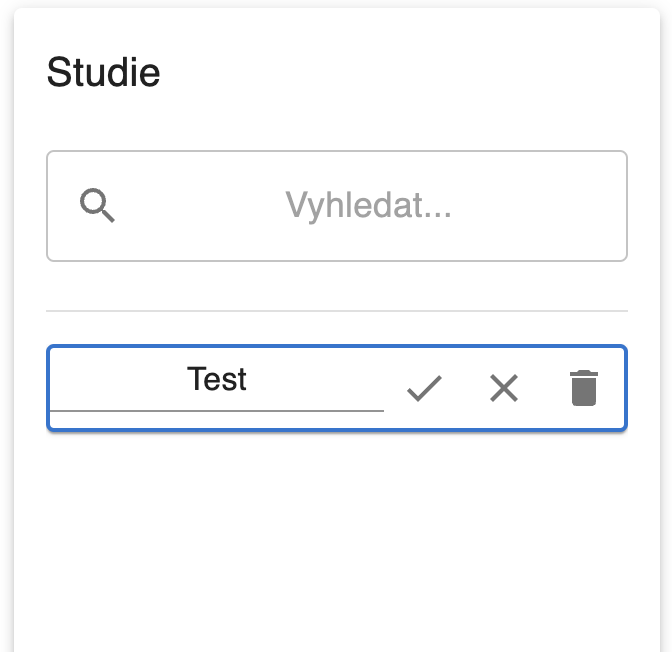
\includegraphics[width=0.45\textwidth]{img/editace-studie/editace_2.png}
        \caption{Režim editace názvu studie s tlačítky pro uložení a zrušení.}
        \label{fig:editace-studie-2}
    \end{figure}

    \item Zadejte nový název studie.
    \item Kliknutím na ikonu \textbf{fajfky} nový název uložíte. Pokud chcete úpravu zrušit bez uložení, klikněte na ikonu \textbf{křížku}.
\end{enumerate}

\subsubsection{Mazání studie}

\begin{enumerate}
    \item V~seznamu studií klikněte u~odpovídající studie na ikonu \textbf{popelnice} (viz Obrázek~\ref{fig:editace-studie-1} nebo Obrázek~\ref{fig:editace-studie-2}).
    \item Zobrazí se potvrzovací dialogové okno s~dotazem, zda si opravdu přejete studii smazat.
    \item Potvrďte smazání kliknutím na tlačítko \textbf{SMAZAT}. Studie bude odstraněna z~databáze. Upozorňujeme, že smazáním studie nedochází k~odstranění samotných pacientů z~databáze, ruší se pouze jejich vazba na danou studii.
\end{enumerate}

\subsection{Přidání pacienta do existující studie}

Pacienta lze do již vytvořené studie zařadit hromadně při vytváření studie (viz podkapitola~\ref{sec:vytvoreni-studie}), nebo individuálně přímo z~karty konkrétního pacienta v~sekci \textbf{Seznam pacientů}.

\subsubsection{Postup při zařazení pacienta z jeho karty}

\begin{enumerate}
    \item \textbf{Otevření karty pacienta}:
    V~levém navigačním menu přejděte do záložky \textbf{Seznam pacientů} a v~prostředním panelu vyhledejte a kliknutím vyberte pacienta, kterého si přejete do studie zařadit.

    \item \textbf{Vyhledání sekce Studie v kartě pacienta}:
    Na hlavní pracovní ploše (v~pravém panelu) sjeďte ve formuláři pacienta dolů až k~sekci \textbf{Studie} (viz Obrázek~\ref{fig:pridani-do-studie-1}).

    \begin{figure}[H]
        \centering
        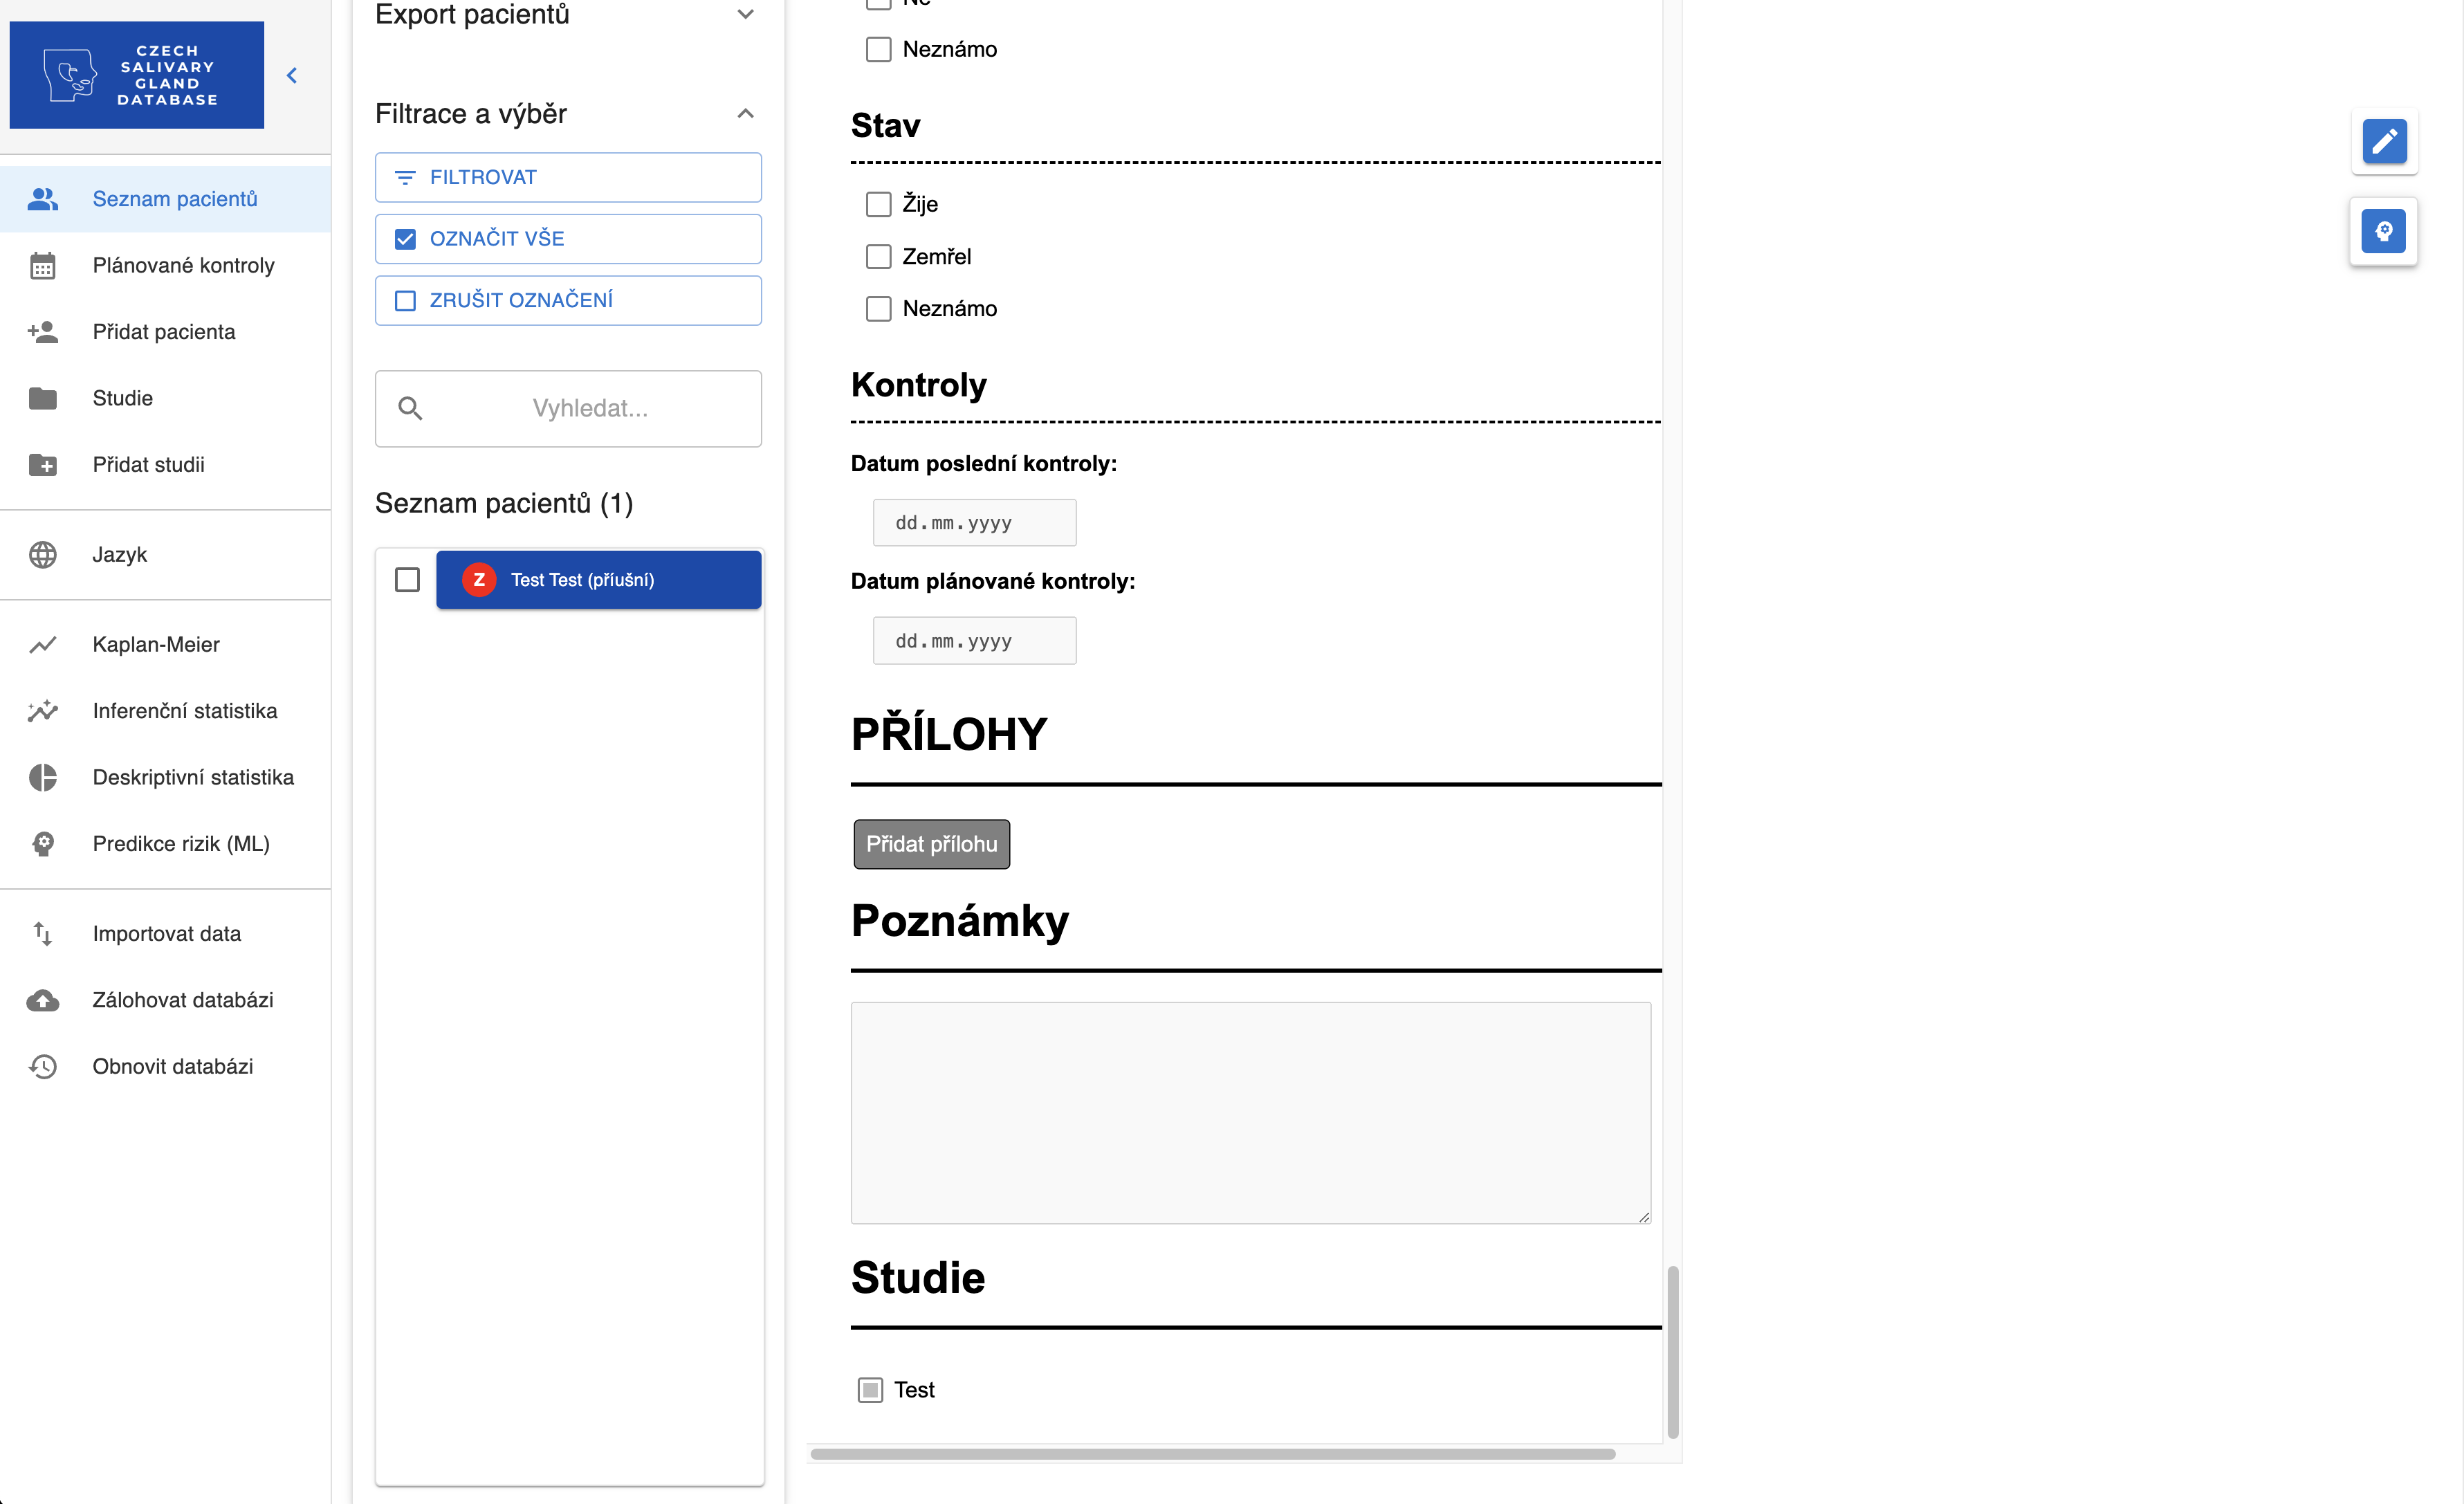
\includegraphics[width=0.85\textwidth]{img/pridani-do-studie/pridani_1.png}
        \caption{Sekce Studie na kartě pacienta s nabídkou dostupných studií.}
        \label{fig:pridani-do-studie-1}
    \end{figure}

    \item \textbf{Zařazení pacienta do studie}:
    V~sekci \textbf{Studie} je zobrazen přehled všech existujících studií odpovídajících dané kategorii. Zaškrtněte políčko (checkbox) u~studie, do které chcete pacienta přiřadit.

    \item \textbf{Uložení změny}:
    Pokud upravujete záznam v~režimu editace, potvrdíte uložení kliknutím na tlačítko \textbf{ULOŽIT ZMĚNY} v~pravé horní liště. Pacient bude automaticky zařazen do vybrané studie a bude se zobrazovat v~jejím přehledu v~záložce \textbf{Studie}.
\end{enumerate}

\section{Zobrazení křivek přežití a recidivy (Kaplan-Meier)}

Aplikace \texttt{csgdb} poskytuje analytický modul pro konstrukci a vizualizaci křivek přežití a recidivy pomocí Kaplan-Meierovy metody.

\begin{enumerate}
    \item V~levém navigačním menu přejděte do části \textbf{Kaplan-Meier}.
    \item V~ovládacím panelu zvolte požadovaný typ analýzy a vydefinujte histopatologické skupiny pacientů, pro které chcete křivky srovnávat (viz Obrázek~\ref{fig:kaplan-meier-1}).

    \begin{figure}[H]
        \centering
        
\includegraphics[width=0.85\textwidth]{img/kaplan-meier/kaplan_meier_1.png}
        \caption{Nastavení modulu Kaplan-Meier pro volbu typu křivky a histopatologických skupin.}
        \label{fig:kaplan-meier-1}
    \end{figure}

    \item Na základě vybraných parametrů se automaticky vykreslí graf Kaplan-Meierových křivek.
    \item \textbf{Podmínky pro zahrnutí pacientů do výpočtu}:
    Výpočet křivek se provádí pouze nad pacienty, kteří mají ve svém záznamu řádně vyplněny všechny potřebné údaje:
    \begin{itemize}
        \item \textbf{Pro křivku přežití}: Vyplněná \textit{Histopatologie}, \textit{Rok diagnózy} a \textit{Datum úmrtí}.
        \item \textbf{Pro křivku recidivy}: Vyplněná \textit{Histopatologie}, \textit{Rok diagnózy} a \textit{Datum prokázání recidivy}.
    \end{itemize}
\end{enumerate}

\section{Inferenční statistika}

Modul \textbf{Inferenční statistika} umožňuje provádět statistické testování hypotéz a ověřovat závislosti či rozdíly mezi jednotlivými klinickými a demografickými proměnnými pacientů uložených v~databázi.

\subsection{Volba statistického testu a nastavení parametrů}

\begin{enumerate}
    \item V~levém navigačním menu přejděte do záložky \textbf{Inferenční statistika}.
    \item V~horní části zvolte požadovaný statistický test (viz Obrázek~\ref{fig:inf-stat-1}):
    \begin{itemize}
        \item \textbf{Chi-kvadrát test} -- test nezávislosti dvou kategoriálních proměnných v~kontingenční tabulce.
        \item \textbf{Fisherův exaktní test} -- přesný test vhodný pro kategoriální data při malém počtu pozorování.
        \item \textbf{T-Test} -- parametrický test pro porovnání průměrů dvou nezávislých skupin spojité proměnné.
        \item \textbf{Mann-Whitney U test} -- neparametrický test pro porovnání rozdělení spojité proměnné ve dvou skupinách.
    \end{itemize}

    \begin{figure}[H]
        \centering
        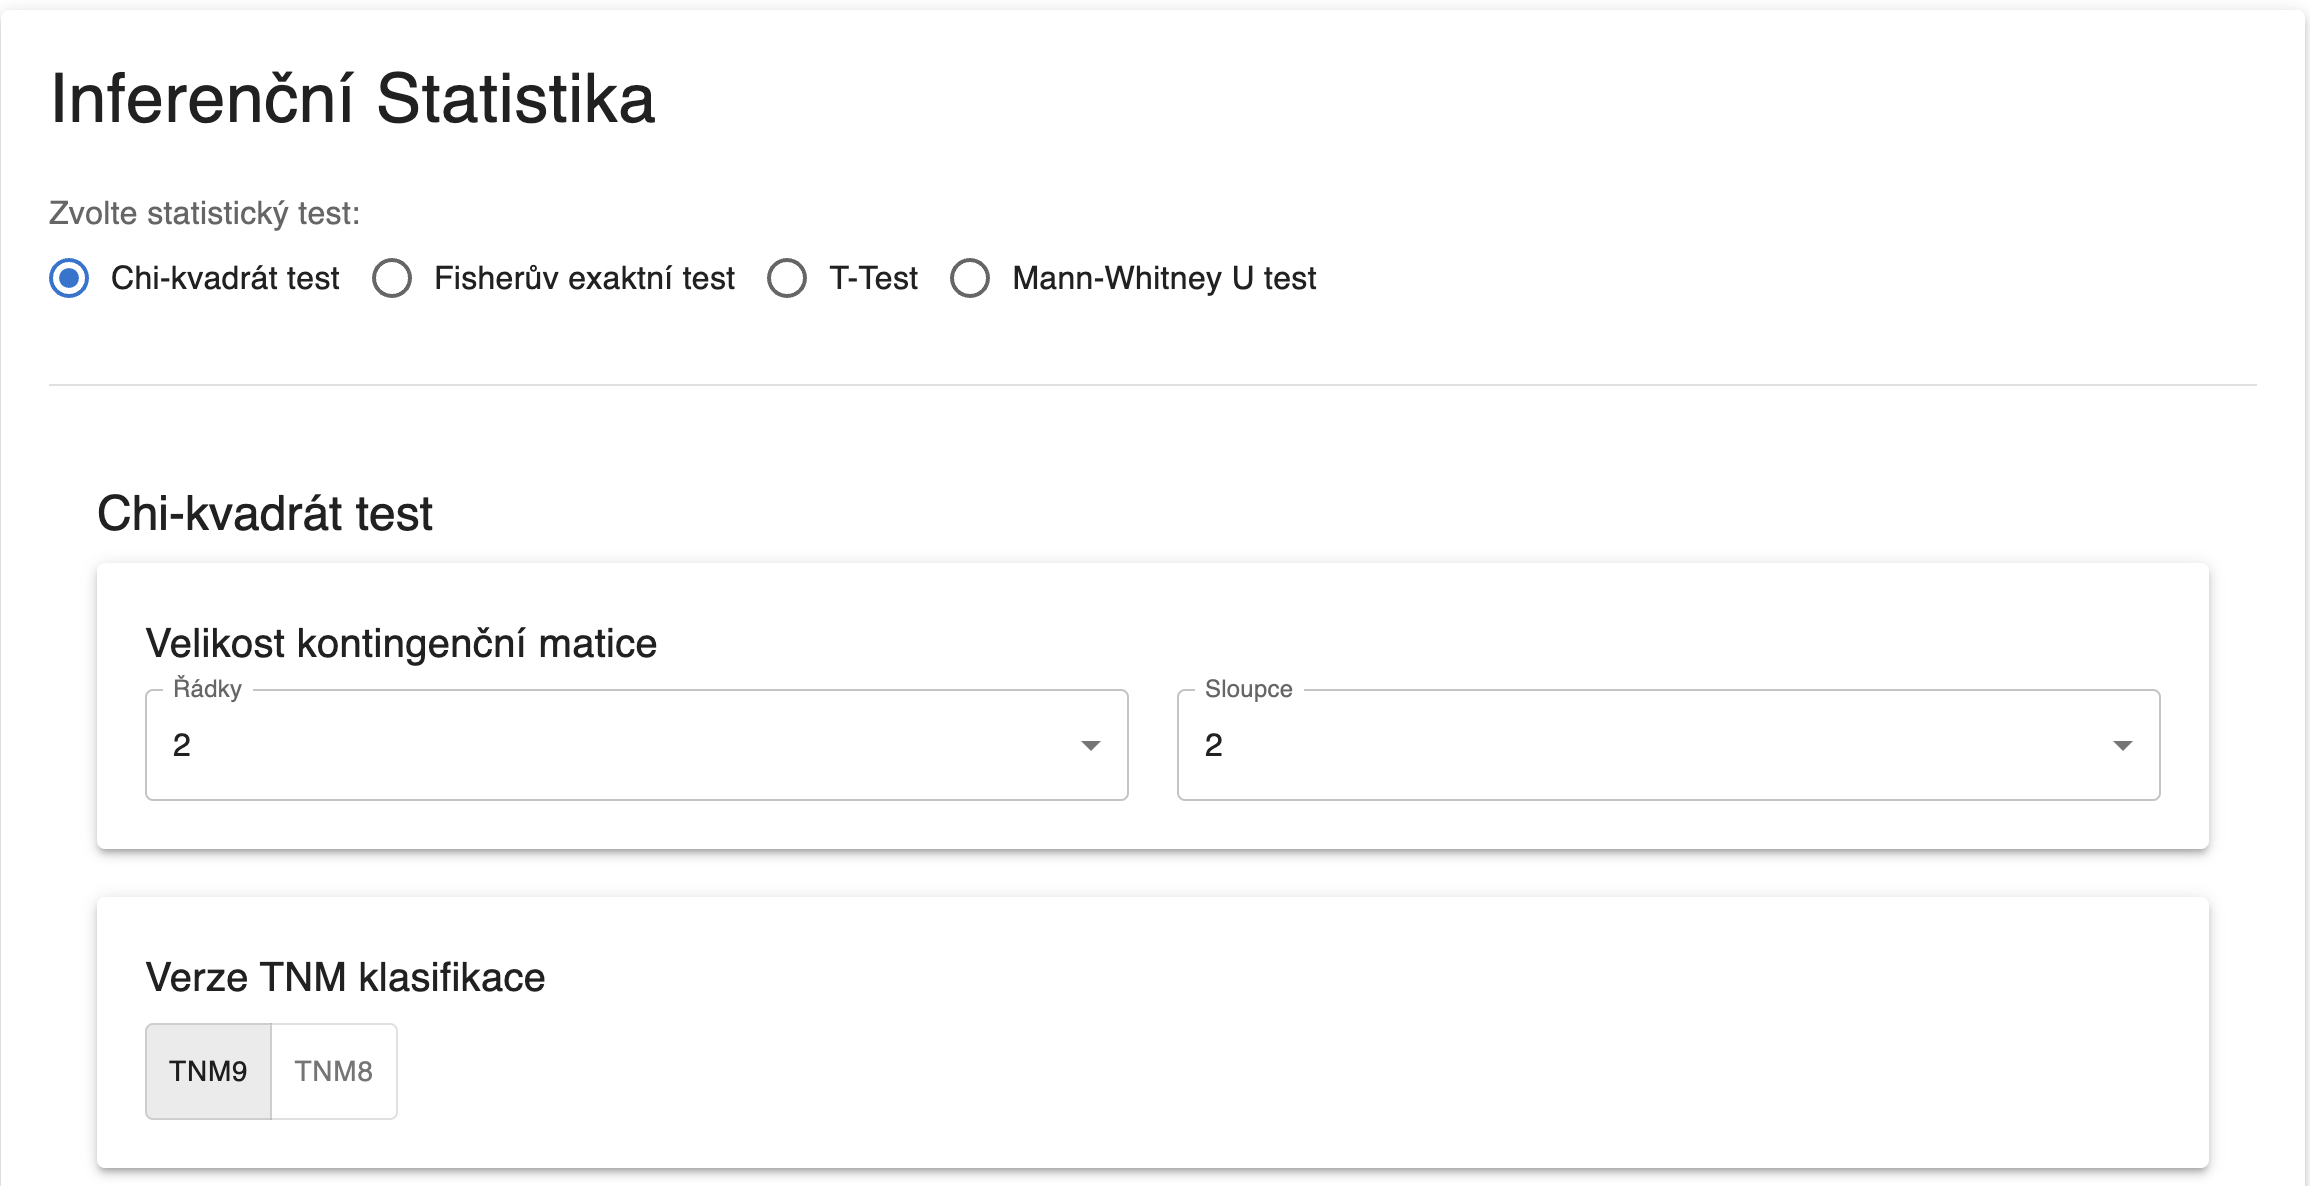
\includegraphics[width=0.85\textwidth]{img/inferencni-statistika/inf_stat_1.png}
        \caption{Výběr statistického testu, rozměrů matice a verze TNM klasifikace.}
        \label{fig:inf-stat-1}
    \end{figure}

    \item Při výběru kontingenčního testu (např. Chi-kvadrát testu) nastavte požadované parametry:
    \begin{itemize}
        \item \textbf{Velikost kontingenční matice}: Zvolte počet řádků a sloupců (např. $2 \times 2$).
        \item \textbf{Verze TNM klasifikace}: Přepněte mezi standardy \texttt{TNM9} a \texttt{TNM8}.
    \end{itemize}
\end{enumerate}

\subsection{Konfigurace řádků a sloupců kontingenční matice}

\begin{enumerate}
    \item \textbf{Definice řádkových kategorií}:
    V~sekci \textit{Vyberte kategorie pro řádky} (viz Obrázek~\ref{fig:inf-stat-2}) vyberte klinickou proměnnou (pomocí záložek: \textit{Histologický typ}, \textit{T klasifikace}, \textit{N klasifikace}, \textit{M klasifikace}, \textit{Perzistence}, \textit{Recidiva}, \textit{Stav pacienta}) a přiřaďte jednotlivé hodnoty do definovaných kategorií řádků.

    \begin{figure}[H]
        \centering
        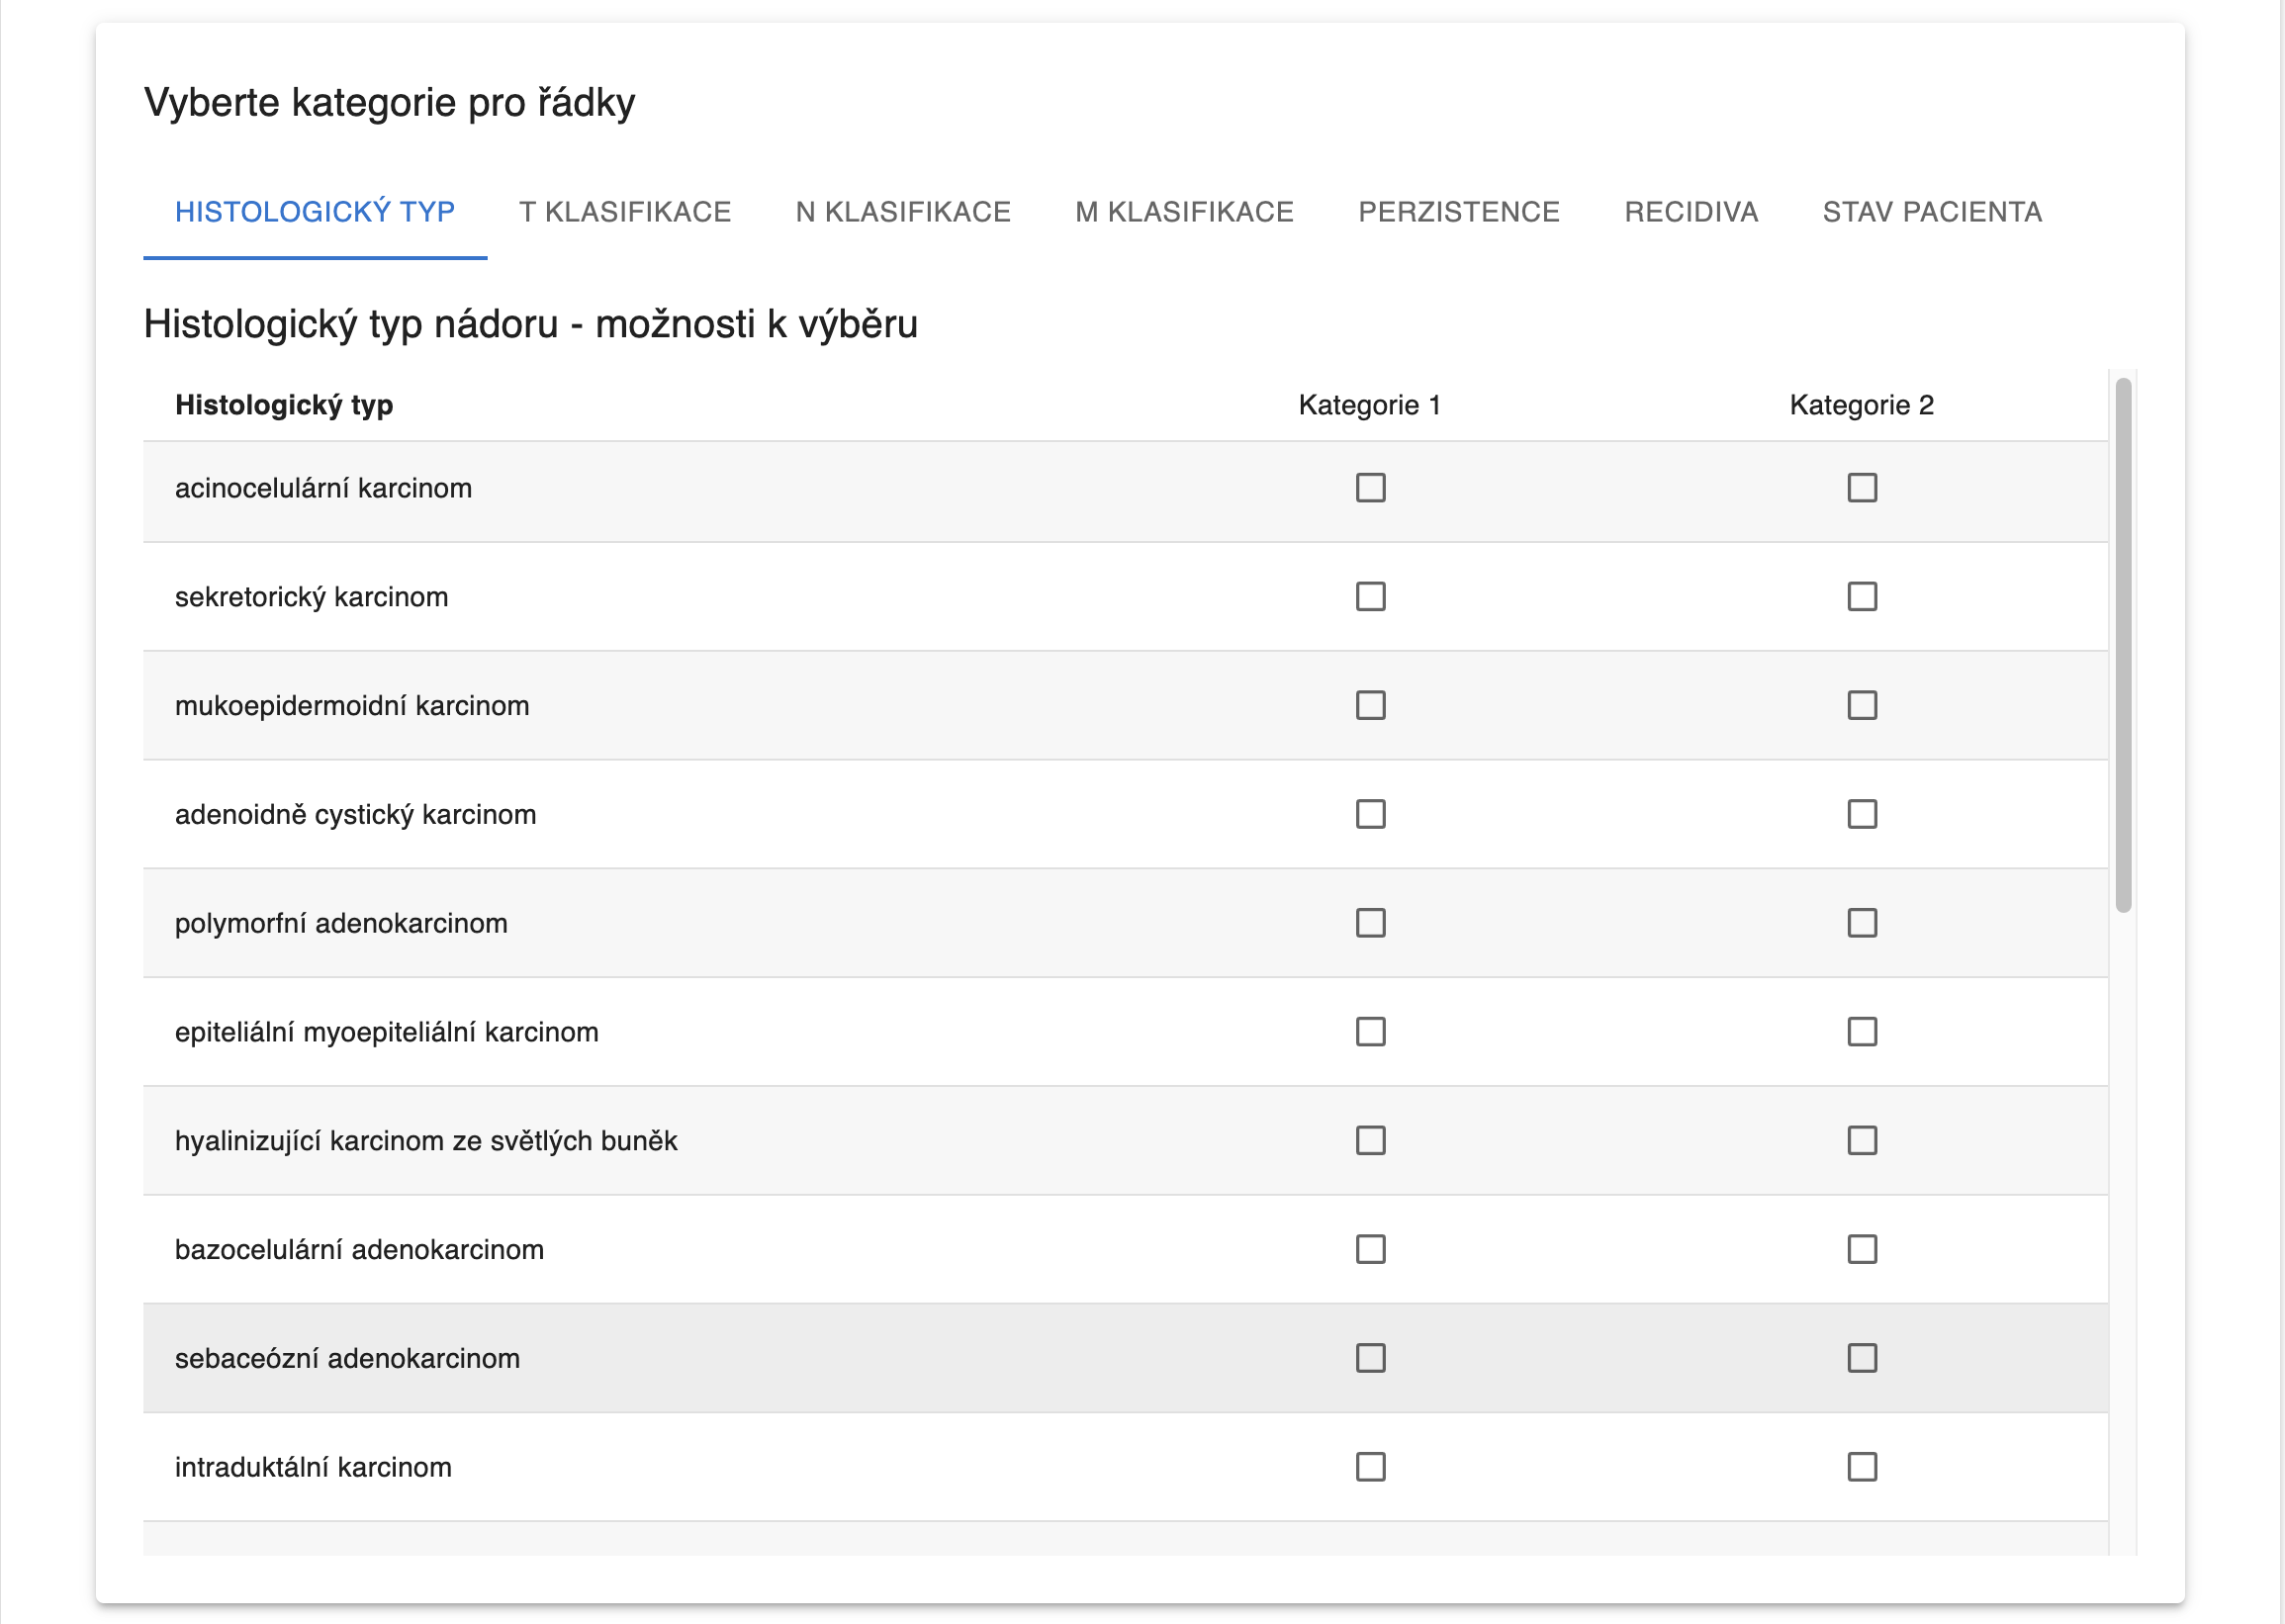
\includegraphics[width=0.85\textwidth]{img/inferencni-statistika/inf_stat_2.png}
        \caption{Přiřazení hodnot klinických proměnných do řádkových kategorií matice.}
        \label{fig:inf-stat-2}
    \end{figure}

    \item \textbf{Definice sloupcových kategorií}:
    V~sekci \textit{Vyberte kategorie pro sloupce} (viz Obrázek~\ref{fig:inf-stat-3}) obdobně zvolte proměnnou a rozřaďte její hodnoty do sloupcových kategorií matice.

    \begin{figure}[H]
        \centering
        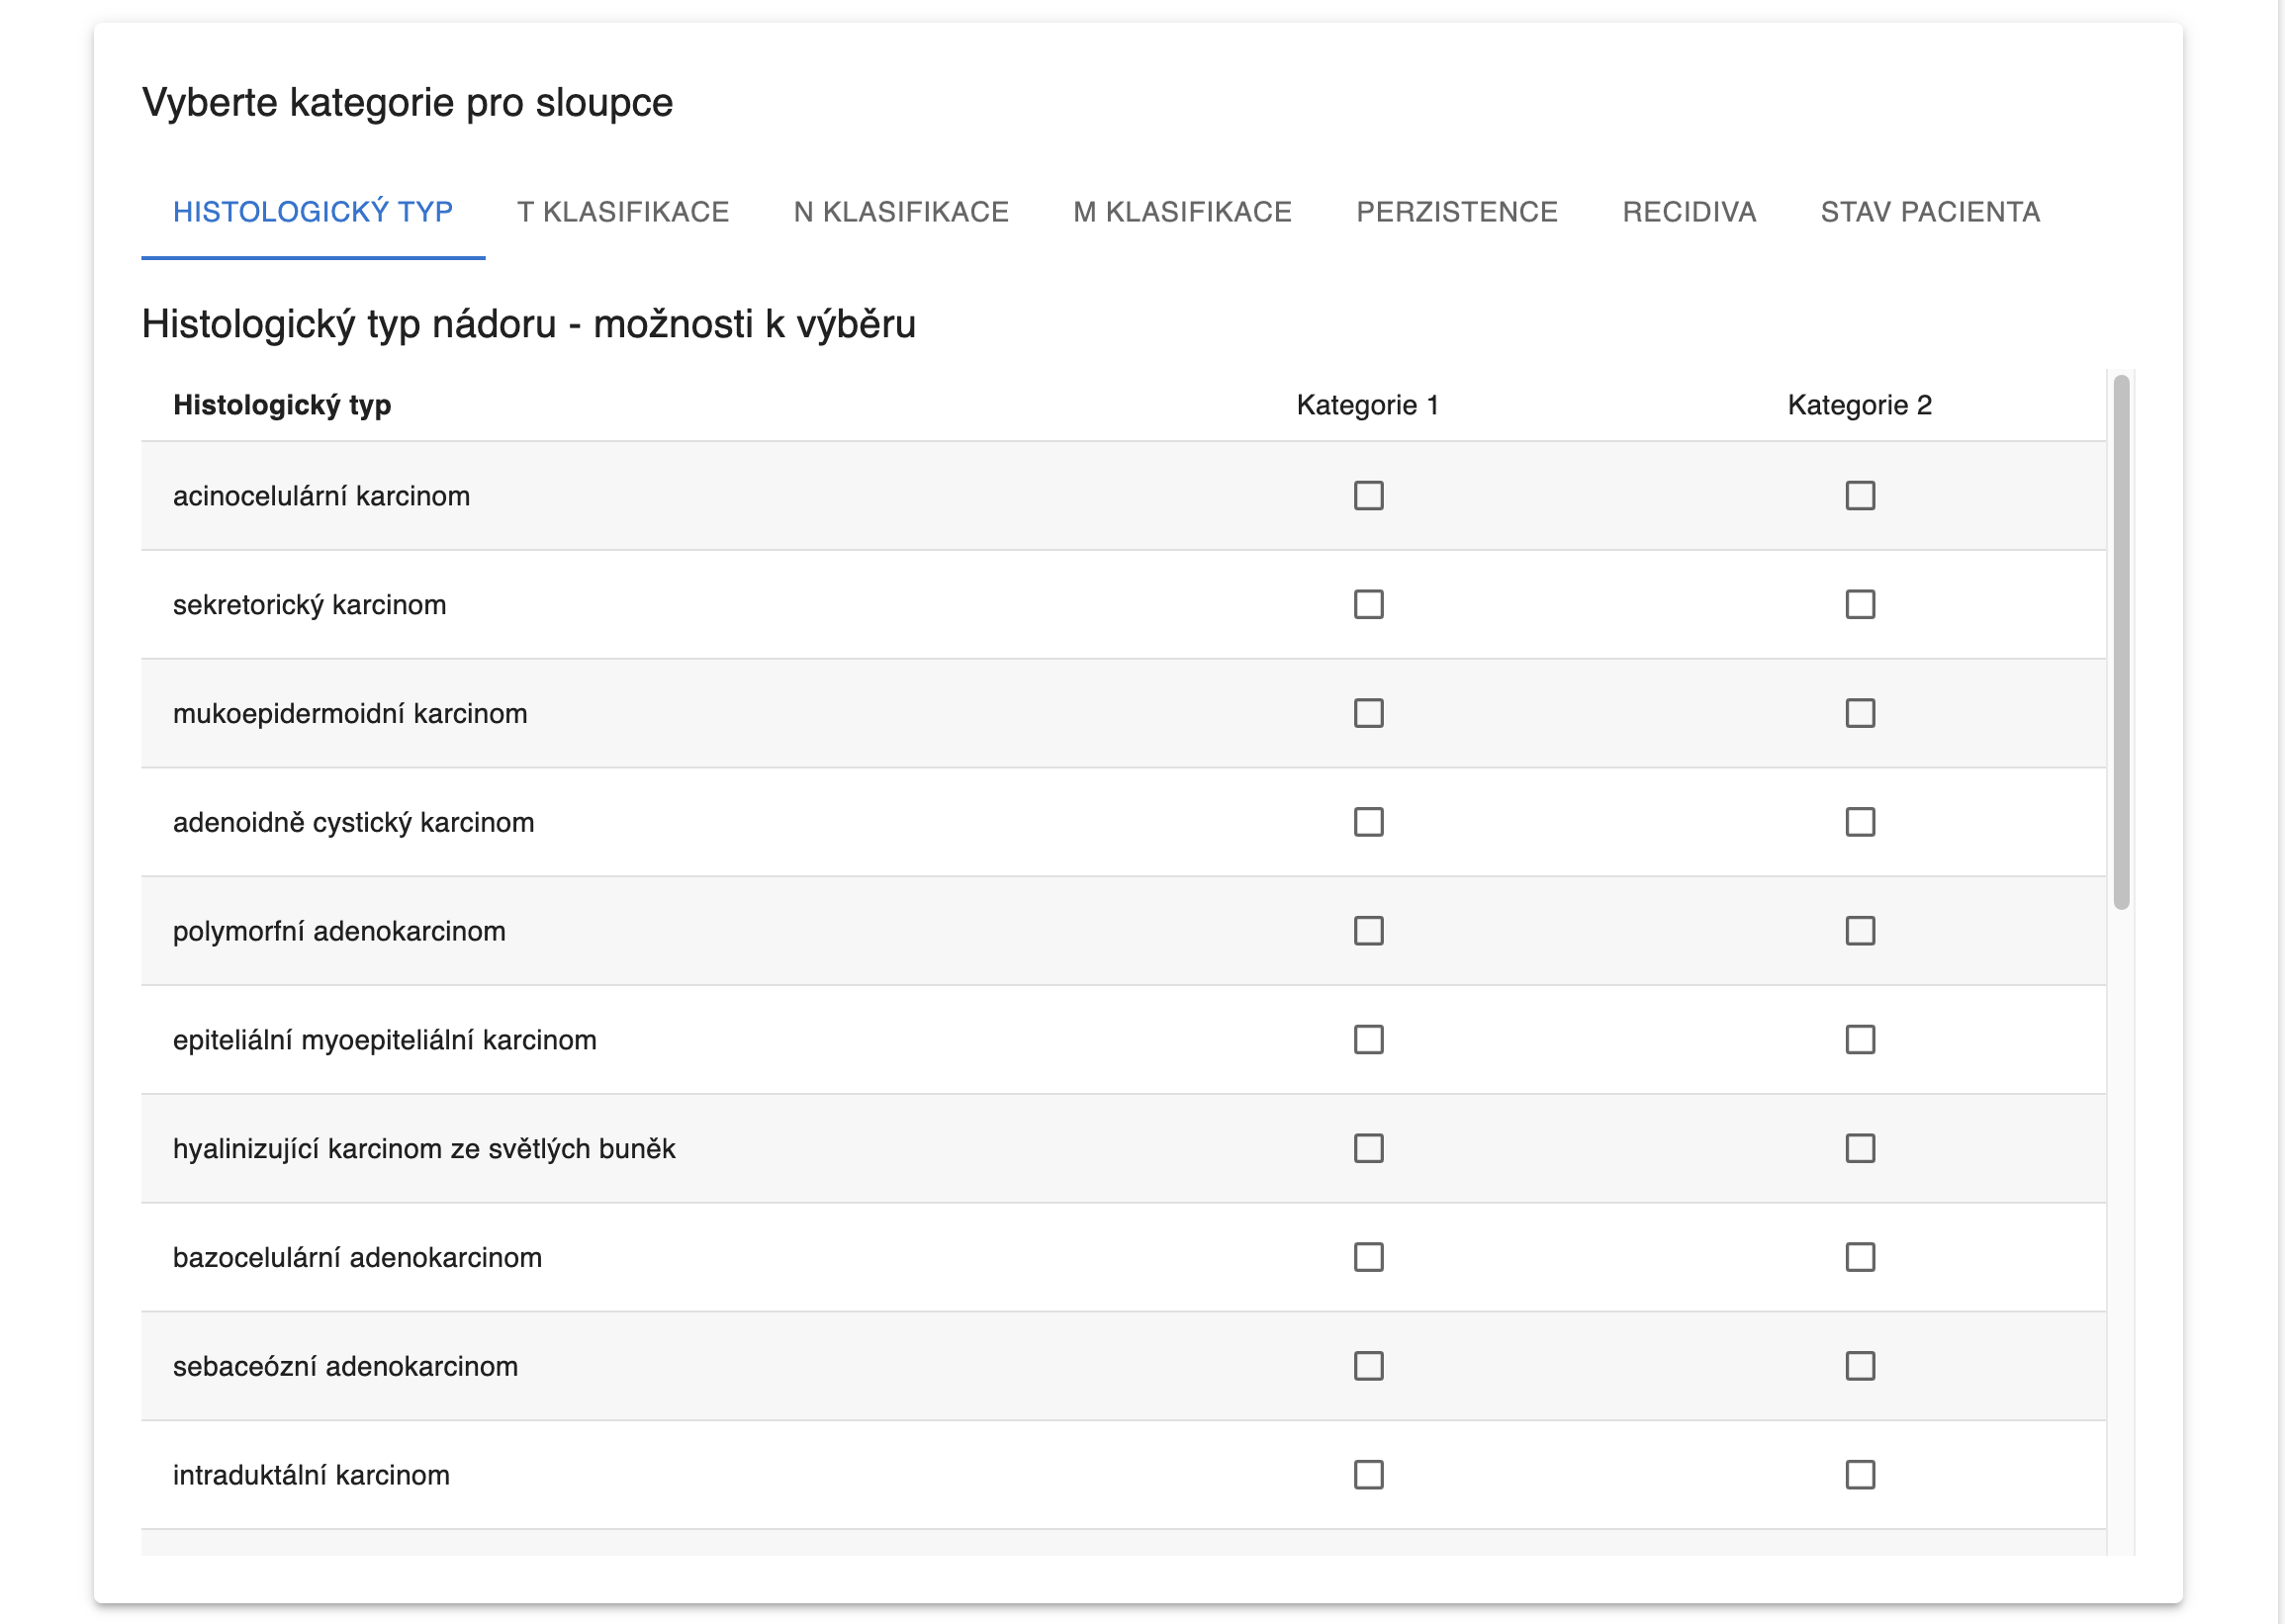
\includegraphics[width=0.85\textwidth]{img/inferencni-statistika/inf_stat_3.png}
        \caption{Přiřazení hodnot do sloupcových kategorií kontingenční matice.}
        \label{fig:inf-stat-3}
    \end{figure}
\end{enumerate}

\subsection{Výpočet a vyhodnocení testu}

\begin{enumerate}
    \item Na základě zadaných kategorií se automaticky vygeneruje \textbf{Kontingenční matice} s~vyplněnými součty (viz Obrázek~\ref{fig:inf-stat-4}).
    \item Nastavte požadovanou \textbf{Hladinu významnosti} v~procentech (výchozí hodnota je $5\,\%$).
    \item Spusťte výpočet stisknutím tlačítka \textbf{VYPOČÍTAT CHI-KVADRÁT} (nebo odpovídajícího tlačítka pro zvolený test). Aplikace spočítá testovou statistiku a p-hodnotu vyhodnocující statistickou významnost.

    \begin{figure}[H]
        \centering
        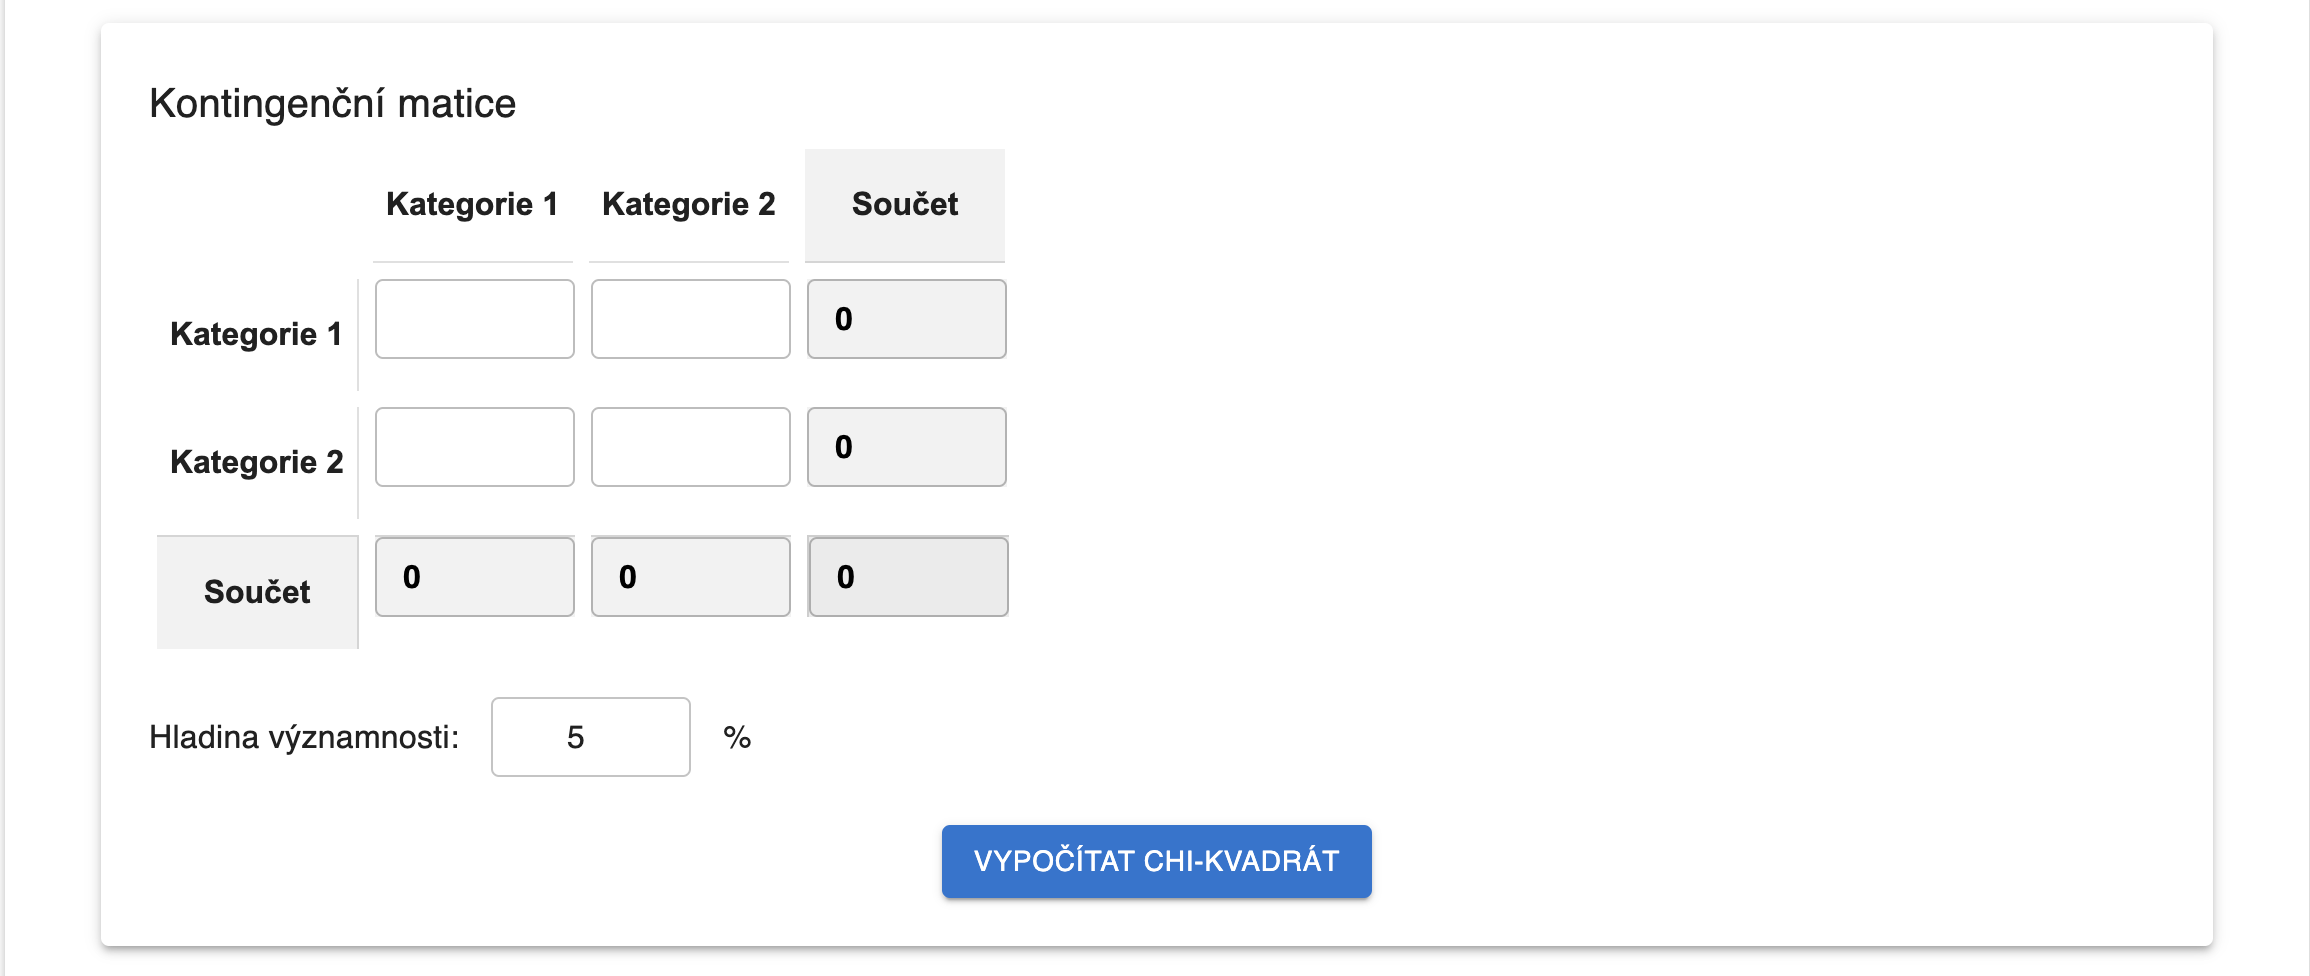
\includegraphics[width=0.85\textwidth]{img/inferencni-statistika/inf_stat_4.png}
        \caption{Kontingenční matice s nastavením hladiny významnosti a tlačítkem pro výpočet testu.}
        \label{fig:inf-stat-4}
    \end{figure}
\end{enumerate}

\section{Deskriptivní statistika}

Modul \textbf{Deskriptivní statistika} slouží k~základnímu sumarizačnímu přehledu a popisu datového souboru pacientů uložených v~databázi. 

Umožňuje uživateli přehledně zobrazit distribuci jednotlivých klinických, histopatologických a demografických parametrů (např. věkové rozložení pacientů, zastoupení jednotlivých typů nádorů, poměr pohlaví nebo stav TNM klasifikace) bez nutnosti provádět složité hypotetické testování. 

\section{Prognostický modul (Predikce rizik ML)}

Prognostický modul v~aplikaci \texttt{csgdb} využívá pokročilé algoritmy strojového učení (např. \textit{Random Survival Forest} a \textit{Cox Proportional Hazards}) k~výpočtu individualizovaného rizikového skóre přežití nebo recidivy pacienta.

\subsection{Výpočet predikce pro pacienta}

\begin{enumerate}
    \item Přejděte do části \textbf{Seznam pacientů} a kliknutím vyberte pacienta, pro kterého chcete vypočítat prognostické skóre.
    \item V~pravém horním rohu pracovní plochy klikněte na modrou ikonu hlavy s~ozubeným kolem (viz Obrázek~\ref{fig:predikce-vypocet-1}).

    \begin{figure}[H]
        \centering
        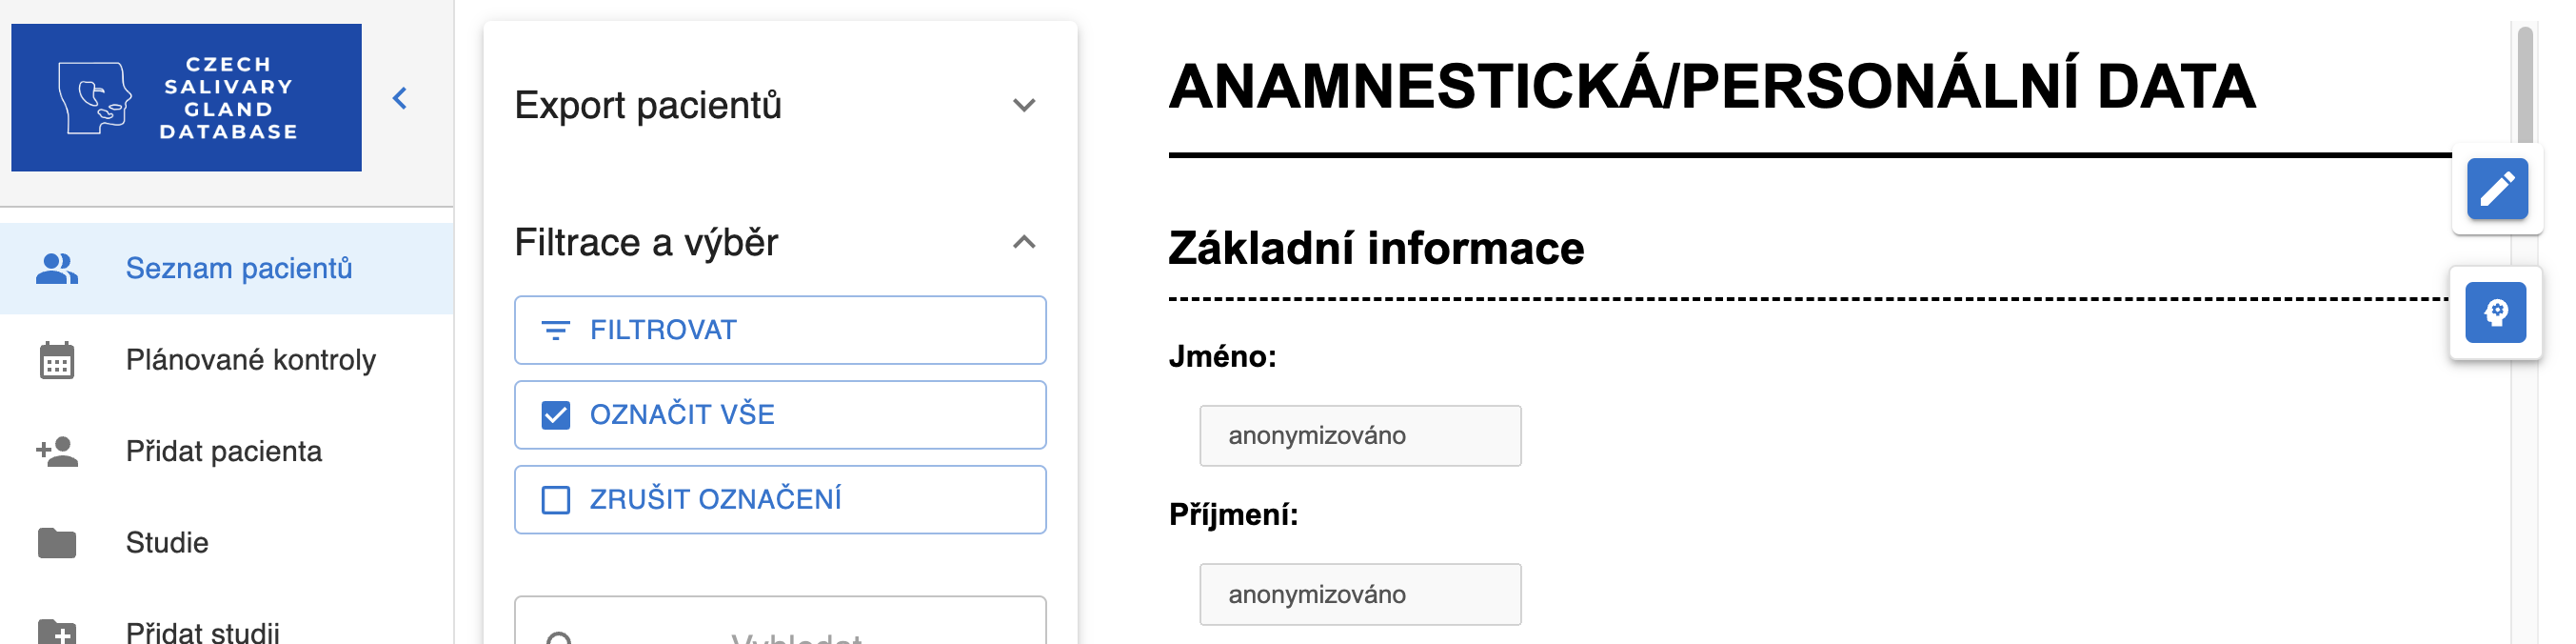
\includegraphics[width=0.85\textwidth]{img/prognosticky-modul/predikce_vypocet_1.png}
        \caption{Ikona pro spuštění výpočtu prognostického skóre u pacienta.}
        \label{fig:predikce-vypocet-1}
    \end{figure}

    \item V~otevřeném okně \textit{Analýza rizika (ML)} zvolte cílovou proměnnou (\textbf{Přežití} nebo \textbf{Recidiva}) a požadovaný algoritmus (např. \textit{Random Survival Forest} či \textit{Cox PH}) (viz Obrázek~\ref{fig:predikce-vypocet-2}).

    \begin{figure}[H]
        \centering
        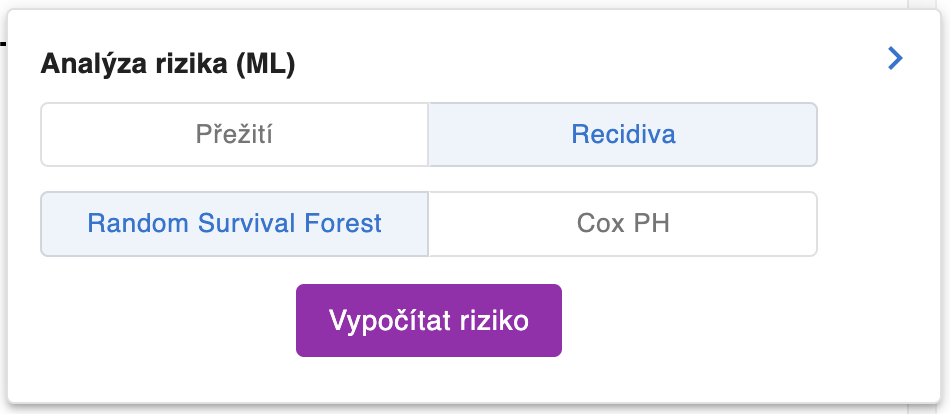
\includegraphics[width=0.55\textwidth]{img/prognosticky-modul/predikce_vypocet_2.png}
        \caption{Volba cílové proměnné a algoritmu pro výpočet predikce.}
        \label{fig:predikce-vypocet-2}
    \end{figure}

    \item Klikněte na fialové tlačítko \textbf{Vypočítat riziko}.
    \item Aplikace provede výpočet a zobrazí výsledky (viz Obrázek~\ref{fig:predikce-vypocet-3}):
    \begin{itemize}
        \item Celkovou kategorializaci rizika (např. \textit{Nízké riziko}),
        \item Odhadovanou pravděpodobnost v~čase (např. pravděpodobnost bez recidivy v~horizontu 1 roku, 3 let a 5 let),
        \item Hlavní rizikové faktory ovlivňující výsledek (např. věk při diagnóze, lymfatická invaze).
    \end{itemize}

    \begin{figure}[H]
        \centering
        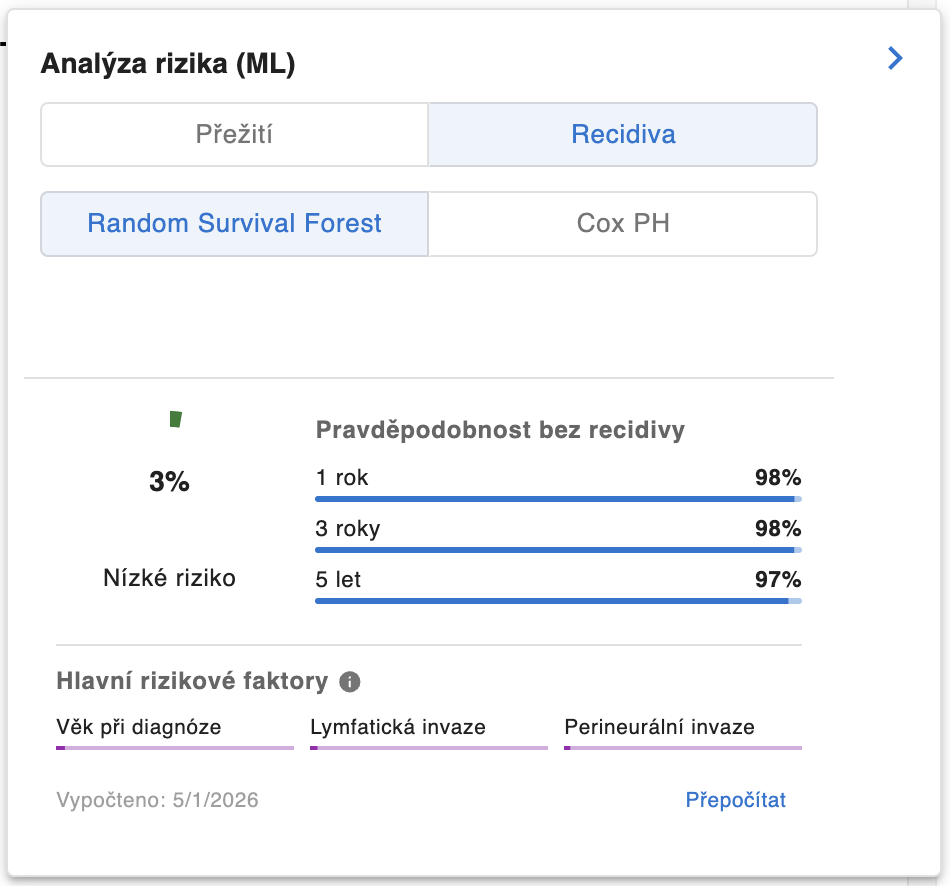
\includegraphics[width=0.6\textwidth]{img/prognosticky-modul/predikce_vypocet_3.png}
        \caption{Zobrazení vypočítané predikce rizika a klíčových faktorů.}
        \label{fig:predikce-vypocet-3}
    \end{figure}
\end{enumerate}

\subsection{Trénování nového modelu}

Kromě předtrénovaných modelů umožňuje aplikace trénovat vlastní prognostické modely nad aktuálními daty v~databázi:

\begin{enumerate}
    \item V~levém navigačním menu přejděte do sekce \textbf{Predikce rizik (ML)}.
    \item Na záložce \textbf{TRÉNOVÁNÍ MODELU} nastavte konfiguraci trénování (viz Obrázek~\ref{fig:predikce-trenink-1}):
    \begin{itemize}
        \item \textbf{Cílová proměnná}: \textit{Celkové přežití} nebo \textit{Recidiva},
        \item \textbf{Algoritmus}: \textit{Random Survival Forest} nebo \textit{Cox Proportional Hazards}.
    \end{itemize}

    \begin{figure}[H]
        \centering
        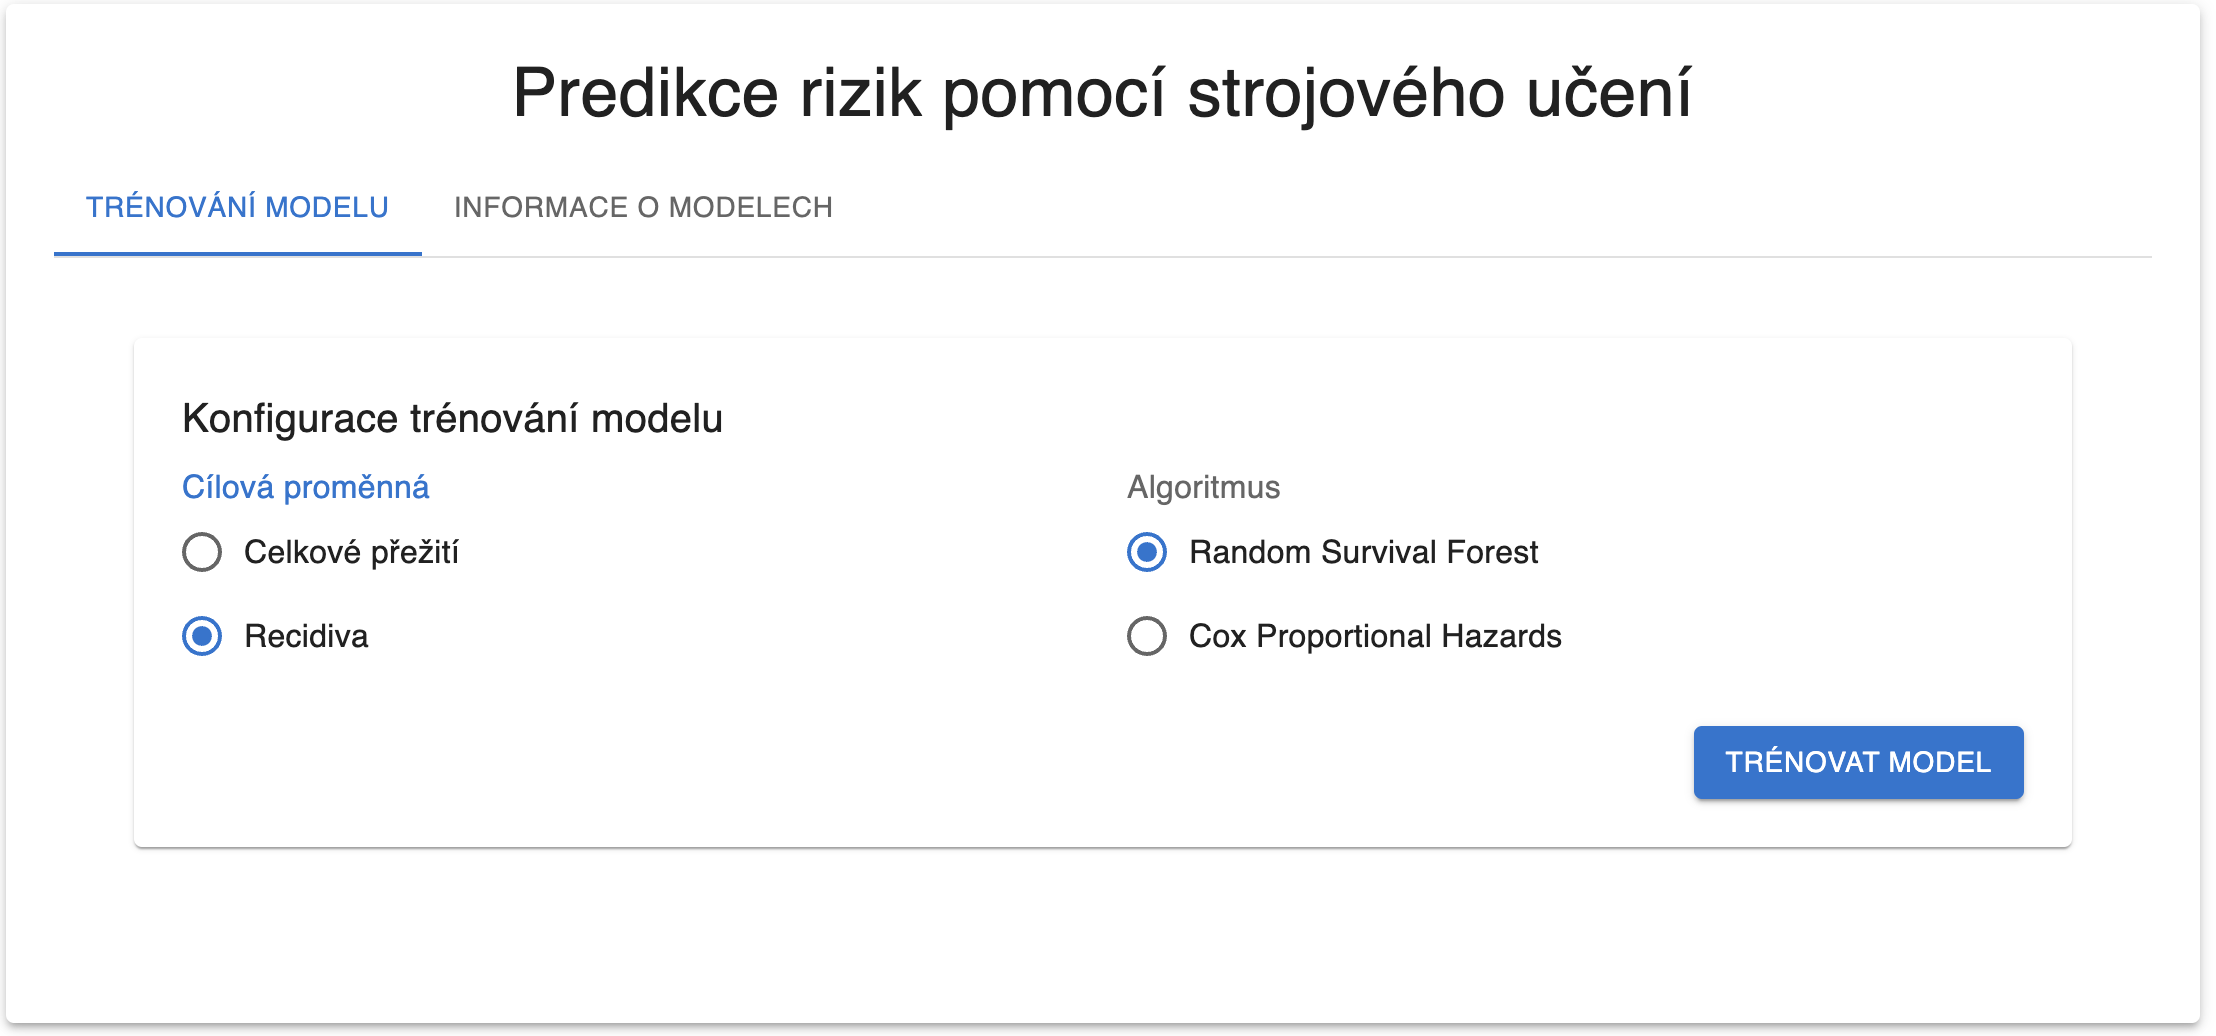
\includegraphics[width=0.85\textwidth]{img/prognosticky-modul/predikce_trenink_1.png}
        \caption{Konfigurace trénování nového prognostického modelu.}
        \label{fig:predikce-trenink-1}
    \end{figure}

    \item Spusťte trénování kliknutím na tlačítko \textbf{TRÉNOVAT MODEL}.
    \item Po dokončení tréninku se v~dolní části zobrazí statistické vyhodnocení modelu (Bootstrap C-index, C-index pro trénovací data, počet použitých pacientů a událostí) (viz Obrázek~\ref{fig:predikce-trenink-2}).

    \begin{figure}[H]
        \centering
        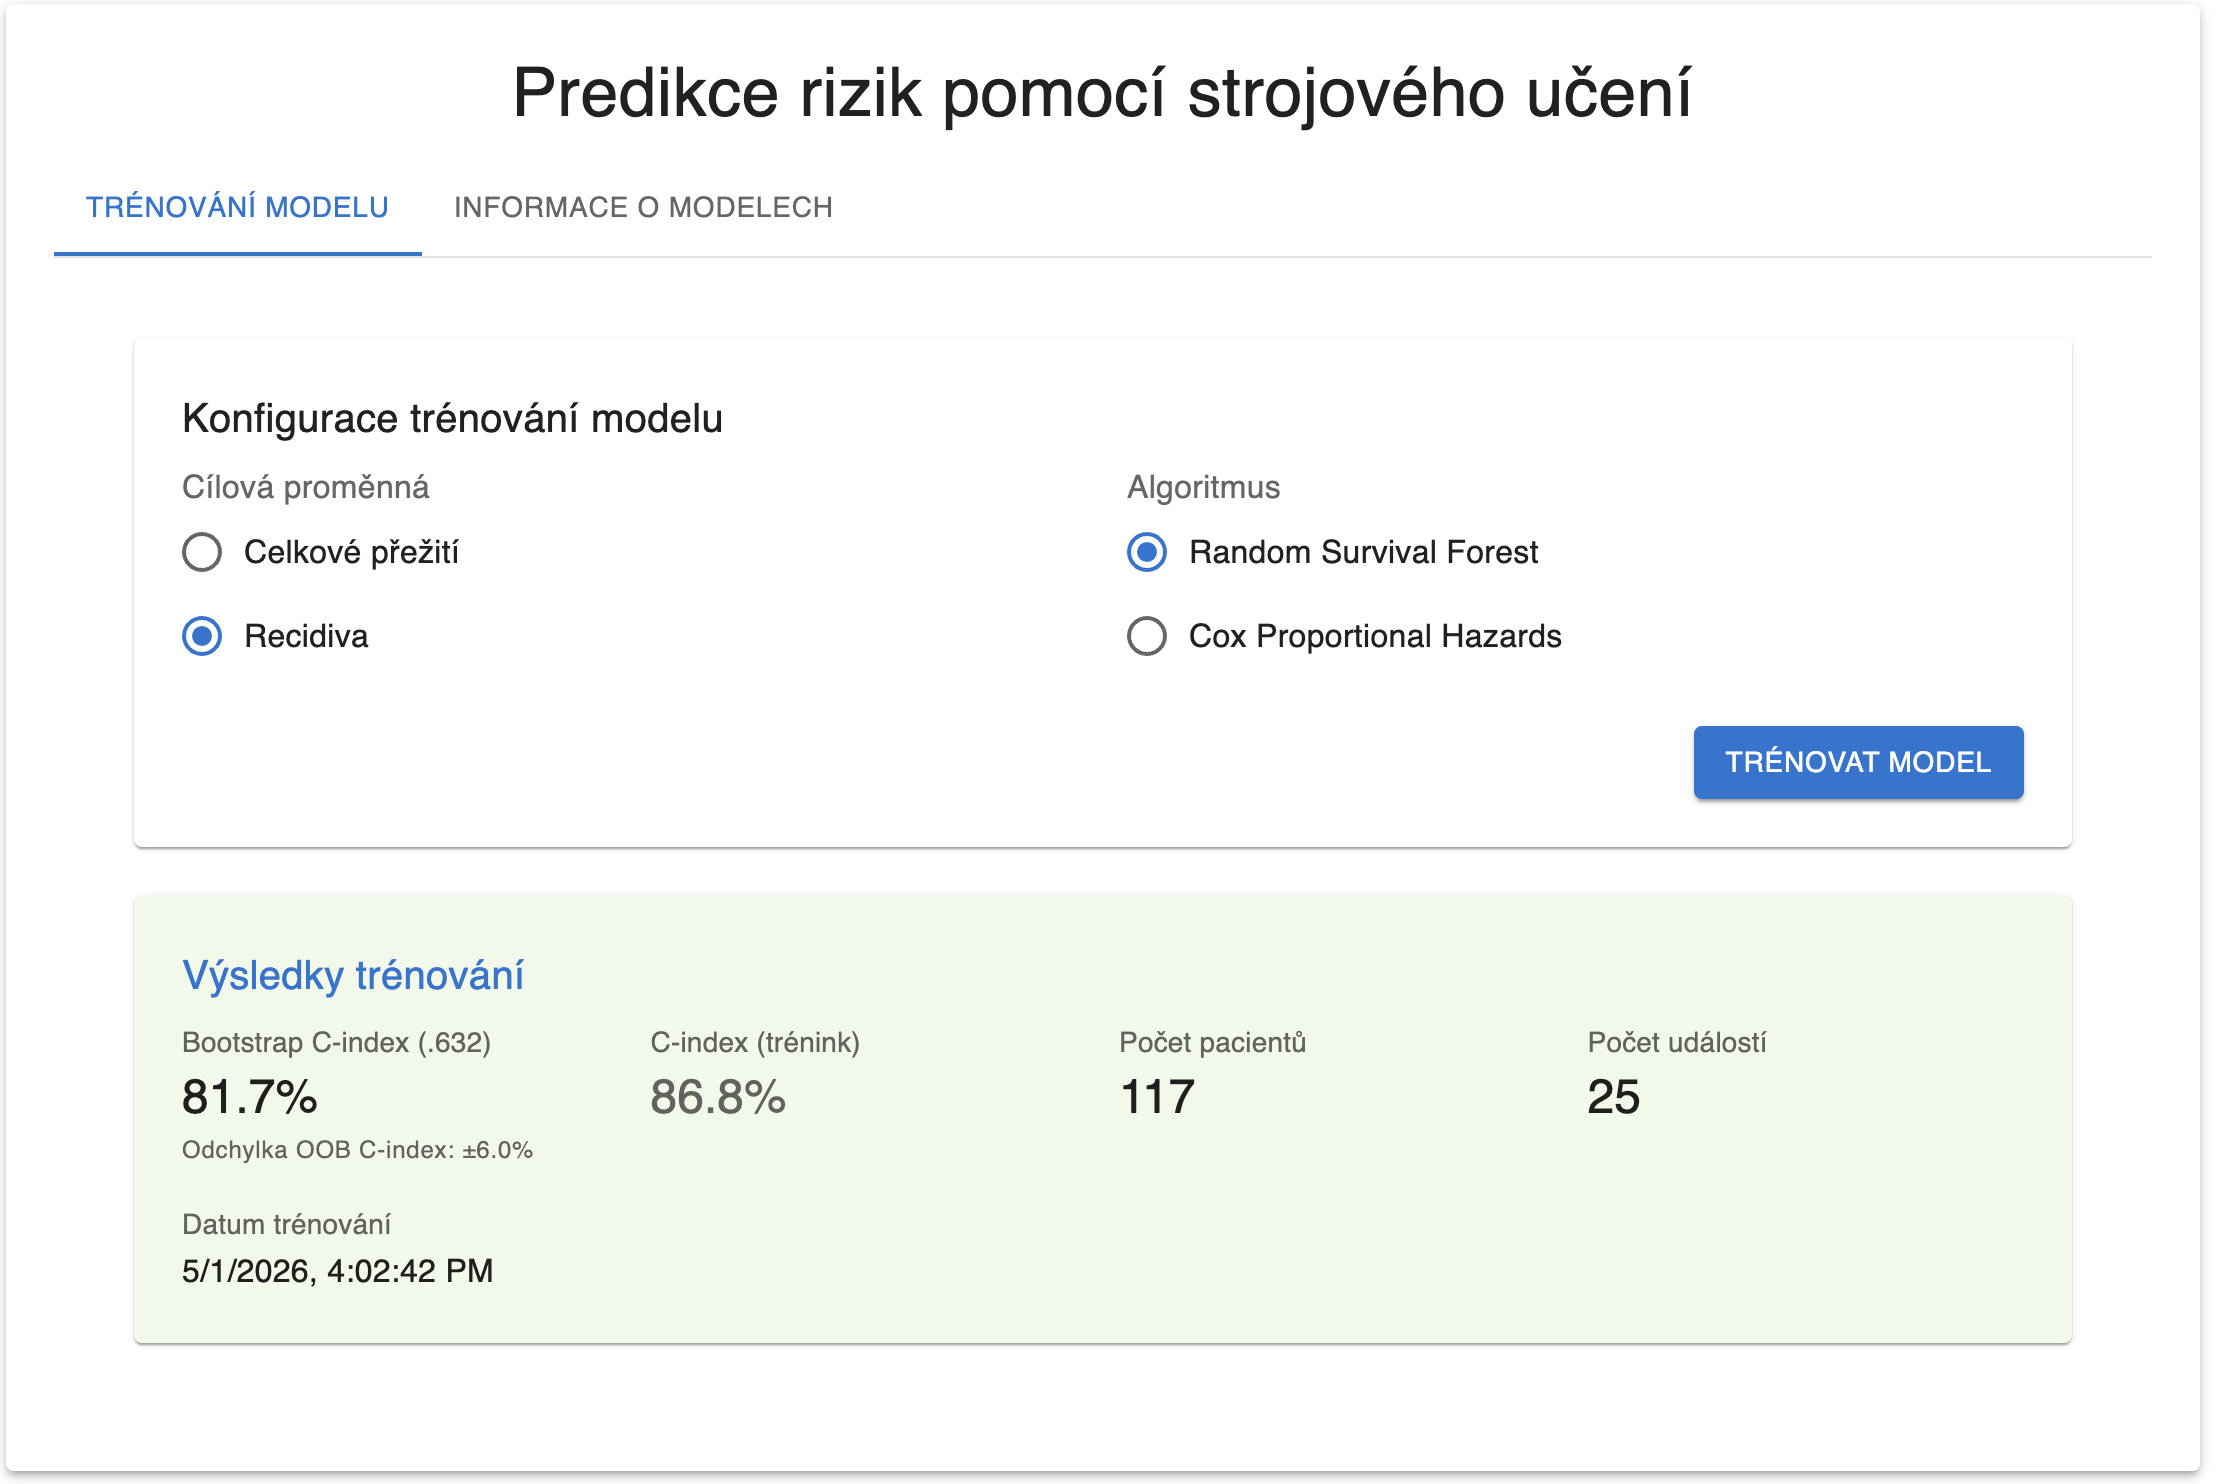
\includegraphics[width=0.85\textwidth]{img/prognosticky-modul/predikce_trenink_2.png}
        \caption{Výsledky a metrika přesnosti natrénovaného modelu.}
        \label{fig:predikce-trenink-2}
    \end{figure}
\end{enumerate}

\subsection{Informace o modelech a správě}

\begin{enumerate}
    \item V~sekci \textbf{Predikce rizik (ML)} přepněte na záložku \textbf{INFORMACE O MODELECH}.
    \item Zobrazí se tabulka všech dostupných (předtrénovaných i~vlastních) modelů v~aplikaci s~podrobnostmi o~jejich přesnosti (C-index) a velikosti trénovacího vzorku (viz Obrázek~\ref{fig:predikce-info}).

    \begin{figure}[H]
        \centering
        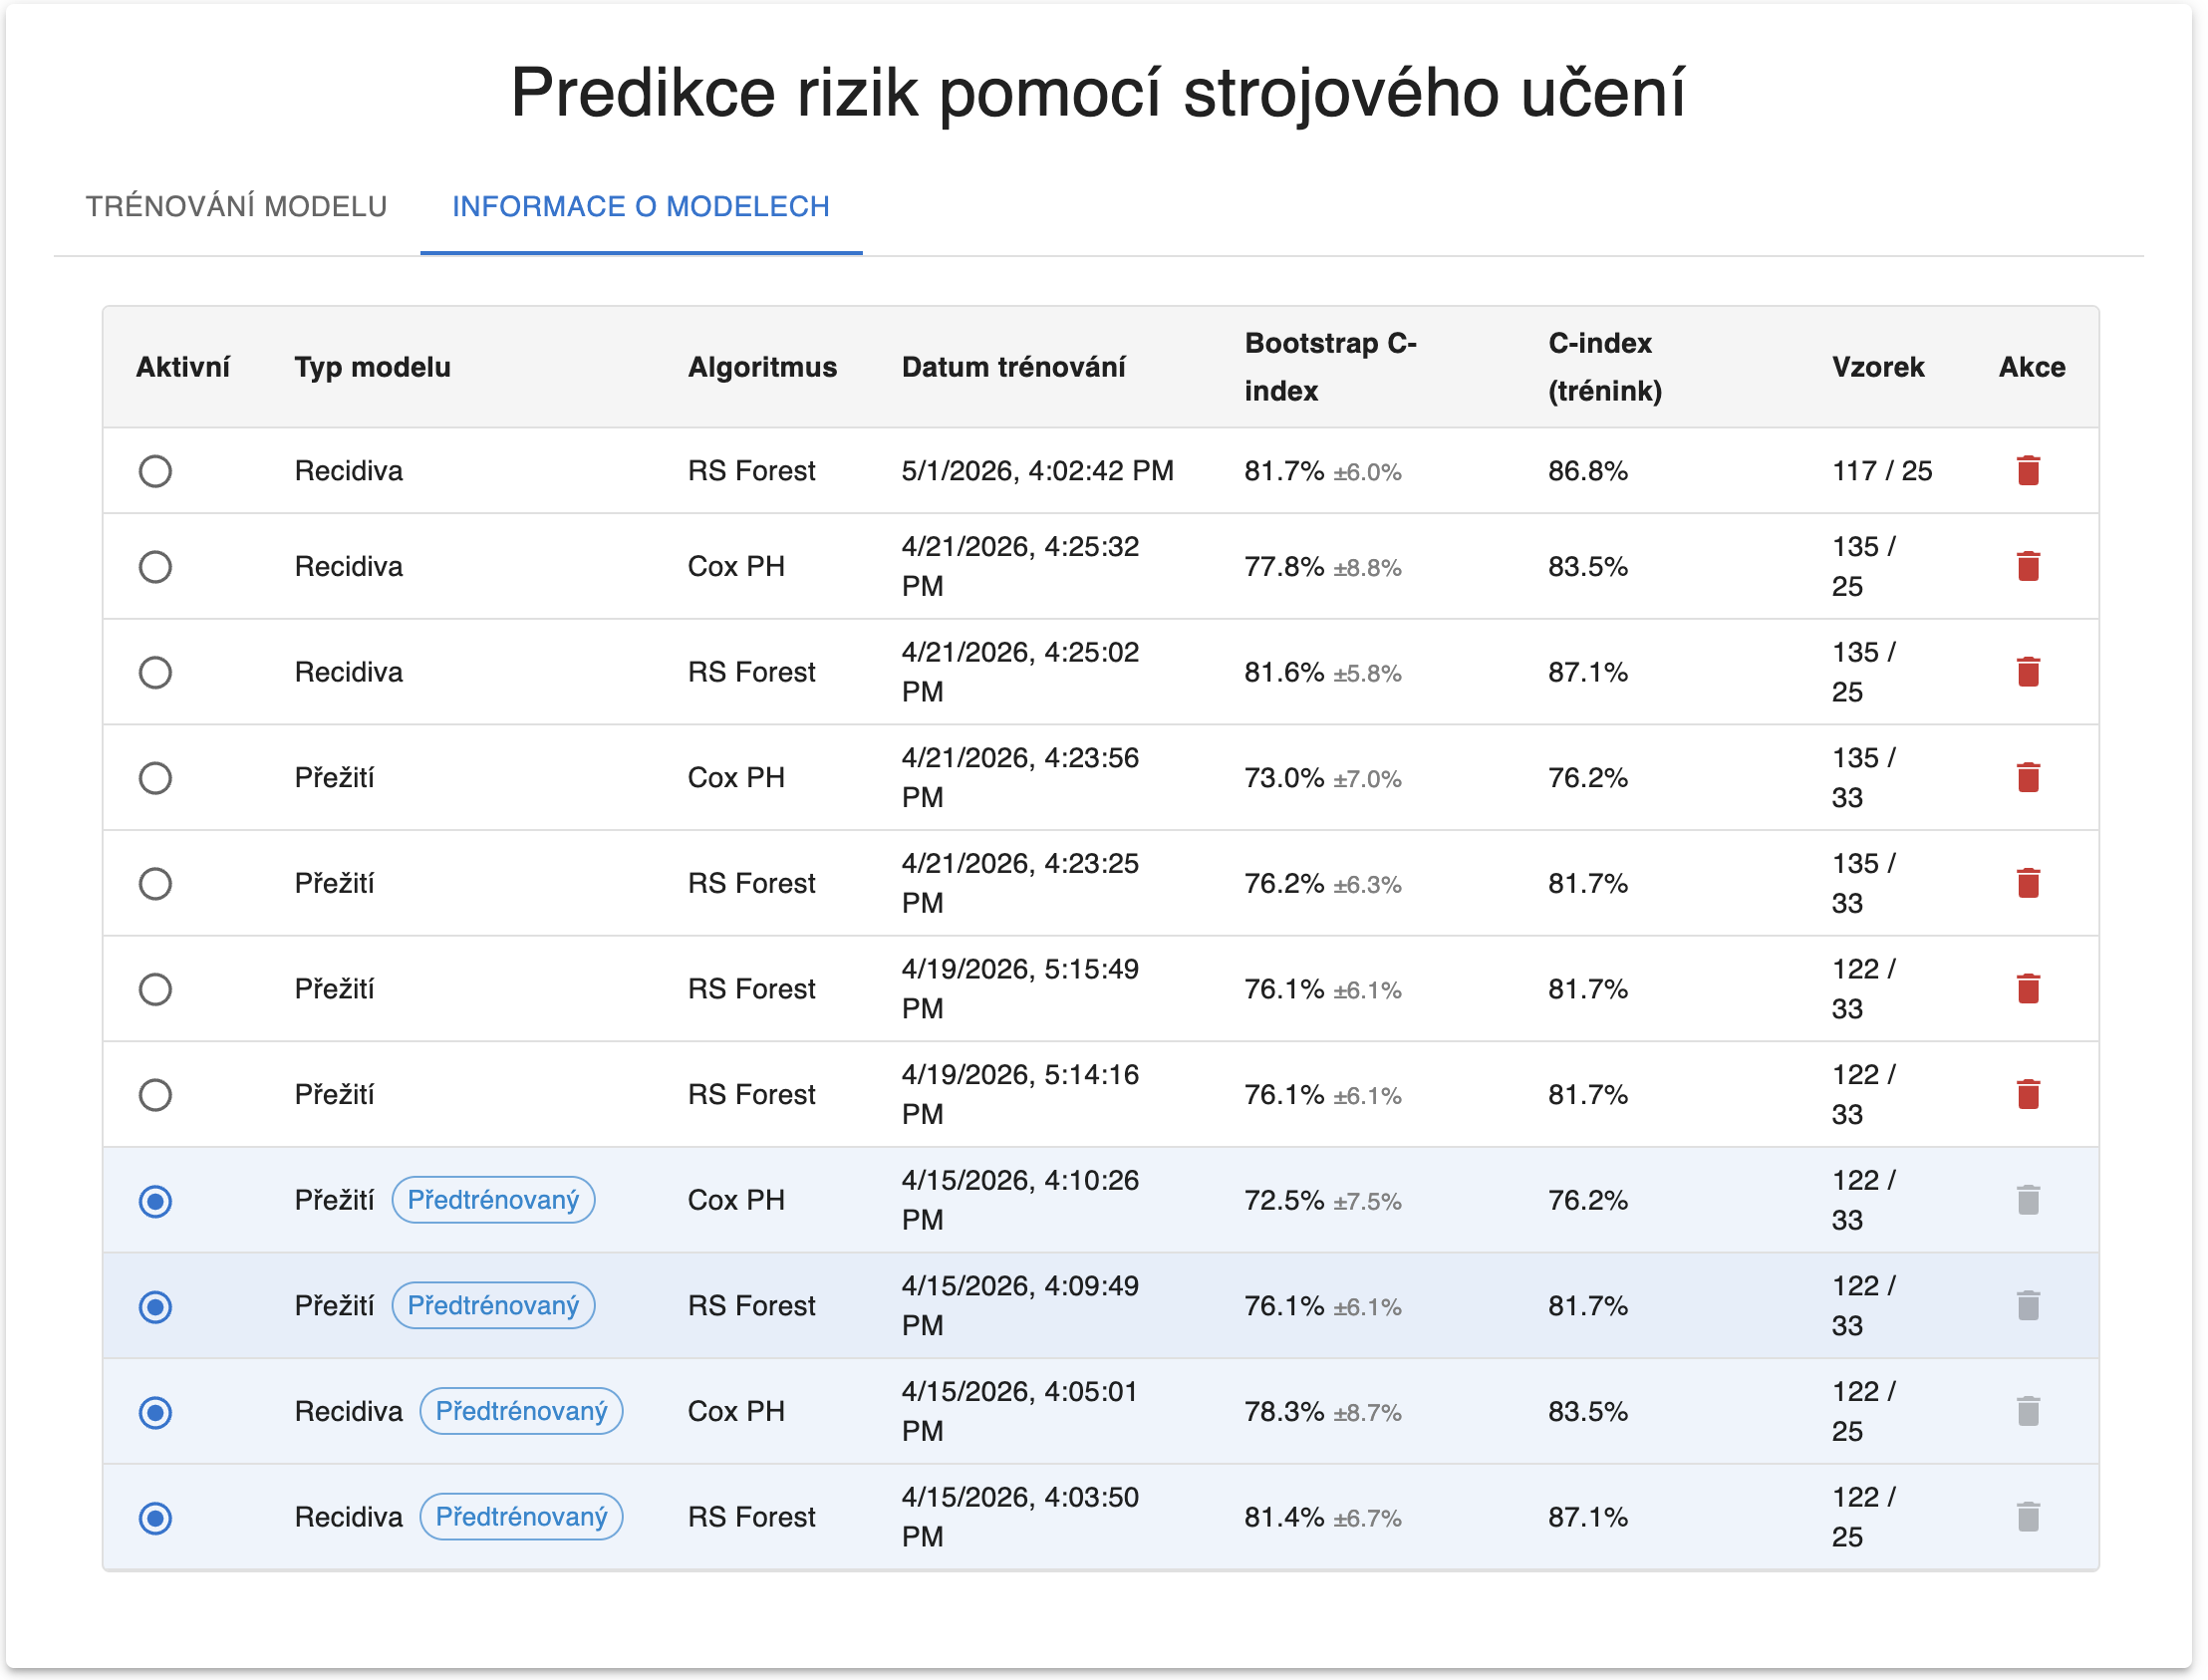
\includegraphics[width=0.9\textwidth]{img/prognosticky-modul/predikce_info.png}
        \caption{Přehled natrénovaných a aktivních modelů s přepínáním a správou.}
        \label{fig:predikce-info}
    \end{figure}

    \item Pomocí přepínačů ve sloupci \textbf{Aktivní} můžete zvolit, které modely mají být primárně využívány pro výpočty u~pacientů. Vlastní natrénované modely lze v~případě potřeby smazat ikona popelnice.
\end{enumerate}

\section{Importování dat}

Pro hromadné nahrávání údajů o~pacientech z~jiných zdrojů či externích souborů slouží modul pro import dat.

\begin{enumerate}
    \item V~levém navigačním menu klikněte na položku \textbf{Importovat data}.
    \item Zobrazí se systémové dialogové okno vašeho operačního systému pro výběr souboru.
    \item Vyhledejte a zvolte datový soubor určený k~importu.
    \item Po potvrzení výchozího souboru se automaticky zahájí zpracování a import pacientů do databáze aplikace.
\end{enumerate}

\section{Zálohování a obnova databáze}

Pro zajištění bezpečnosti dat a ochranu před nechtěnou ztrátou údajů o~pacientech či pro přenos databáze mezi více počítači poskytuje aplikace \texttt{csgdb} vestavěné funkce pro zálohování a obnovení kompletní lokální databáze.

\subsection{Zálohování databáze}

Funkce zálohování vytvoří kompletní kopii aktuálního stavu databáze (včetně všech evidovaných pacientů, vytvořených studií a natrénovaných modelů):

\begin{enumerate}
    \item V~levém navigačním menu klikněte na položku \textbf{Zálohovat databázi}.
    \item Zobrazí se systémové ukládací dialogové okno operačního systému s~předvyplněným názvem záložního souboru (výchozí název \texttt{csgdb\_backup.sqlite}).
    \item Zvolte bezpečnou cílovou složku (např. externí flash disk, síťové úložiště nebo zálohovací adresář).
    \item Kliknutím na tlačítko \textbf{Uložit} aplikace zkopíruje databázový soubor do zvoleného umístění.
\end{enumerate}

\subsection{Obnovení databáze ze zálohy}

Funkce obnovení umožňuje nahradit stávající databázi dříve vytvořenou záložní kopií:

\begin{enumerate}
    \item V~levém navigačním menu klikněte na položku \textbf{Obnovit databázi}.
    \item Zobrazí se systémové dialogové okno pro výběr souboru.
    \item Vyhledejte a vyberte záložní soubor databáze (soubor s~příponou \texttt{.sqlite}).
    \item Po potvrzení výchozího souboru aplikace nahradí pracovní databázi vybraným záložním souborem a automaticky inicializuje databázové schéma a načte uložená data.
\end{enumerate}

\end{document}
